% Allow relative paths in included subfiles that are compiled separately
% See https://tex.stackexchange.com/questions/153312/
\providecommand{\main}{..}
\documentclass[\main/thesis.tex]{subfiles}

\begin{document}

\chapter{Background Information}
\chaptermark{background}
\label{chp:background}

In this chapter, I give a brief overview of the anatomy of a human heart.
Next, I describe the characteristics of a standard 12-lead \gls{ecg} and the notable waves in a \gls{ecg} signal.
I then give an overview of the \emph{PhysioNet/CinC 2020 Challenge} task/objective, provided dataset of \gls{ecg} records, and definitions for the diagnoses we are tasked to predict.

\section{Cardiac Physiology}

\subsection{Anatomy and Electrical Conduction System}
\begin{figure}[ht]
    \centering
    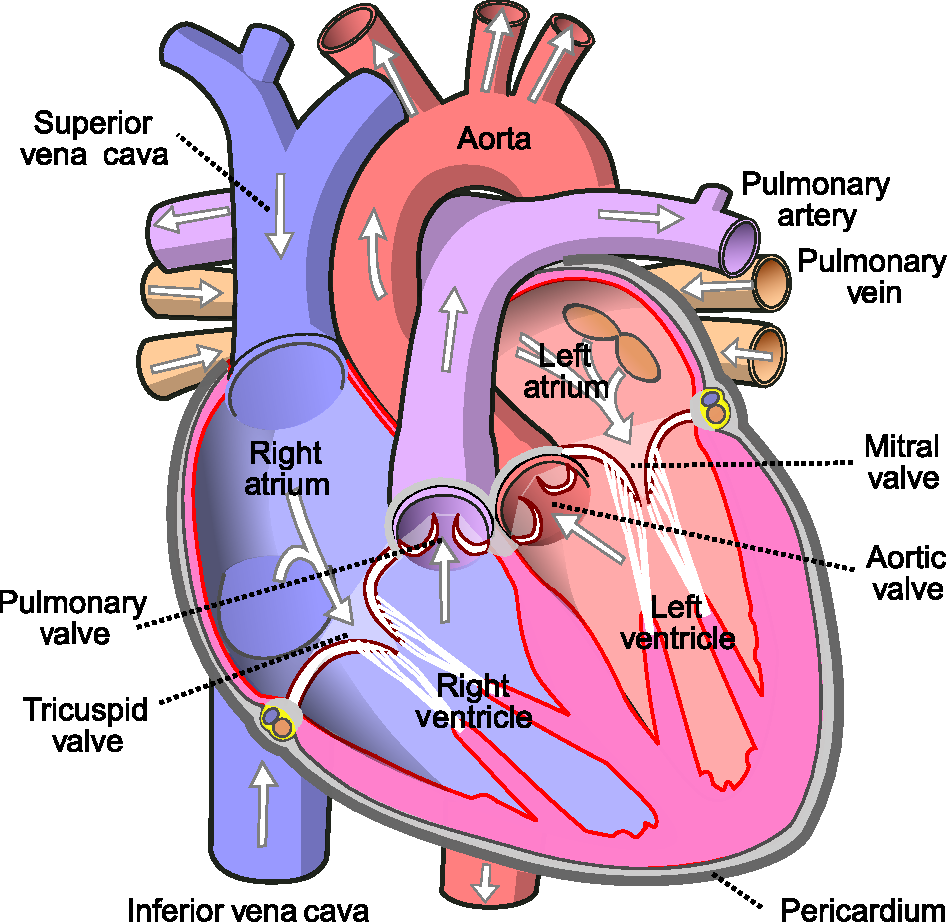
\includegraphics[width=8cm]{figure/Diagram_of_the_human_heart.pdf}
    \caption[Anterior, anatomical view of the structures of a human heart.]{Anterior, anatomical view of a human heart. The primary valves and chambers of the heart are annotated, with arrows indicating the direction of blood flow due to the contractions of the cardiac chambers.
    Image licensed \texttt{CC BY-SA 3.0} from Wikipedia user \href{https://en.wikipedia.org/wiki/User:Wapcaplet}{Wapcaplet}, source: \url{https://en.wikipedia.org/wiki/Heart\#/media/File:Diagram\_of\_the\_human\_heart\_(cropped).svg}.
    }
    \label{fig:heart_anatomy}
\end{figure}

A high level overview of the primary valves and chambers within the heart can be found in Figure~\ref{fig:heart_anatomy}.
The upper chambers of the heart, consisting of the right and left atriums, work in cooperation with the lower chambers of the heart, consisting of the left and right ventricles~\cite{anderson_wilcoxs_2013}.
The right ventricle pushes blood into the pulmonary artery which connects to the lungs to return oxygenated blood~\cite{anderson_wilcoxs_2013}.
The oxygenated blood returns to the heart through the pulmonary veins and enters into the left atrium~\cite{anderson_wilcoxs_2013}.
The left atrium collects and pumps the oxygenated blood into the left ventricle through the mitral valve~\cite{anderson_wilcoxs_2013}.
The left ventricle pumps the oxygenated blood out of the heart to the rest of the body through the aorta~\cite{anderson_wilcoxs_2013}.
The deoxygenated blood is collected back into the heart through the superior and inferior vena cava and into the right atrium~\cite{anderson_wilcoxs_2013}.
The cycle repeats as the right atrium pumps the blood into the right ventricle through the tricuspid valve, allowing the lungs to once again oxygenate the blood~\cite{anderson_wilcoxs_2013}.

\begin{figure}[ht]
    \centering
    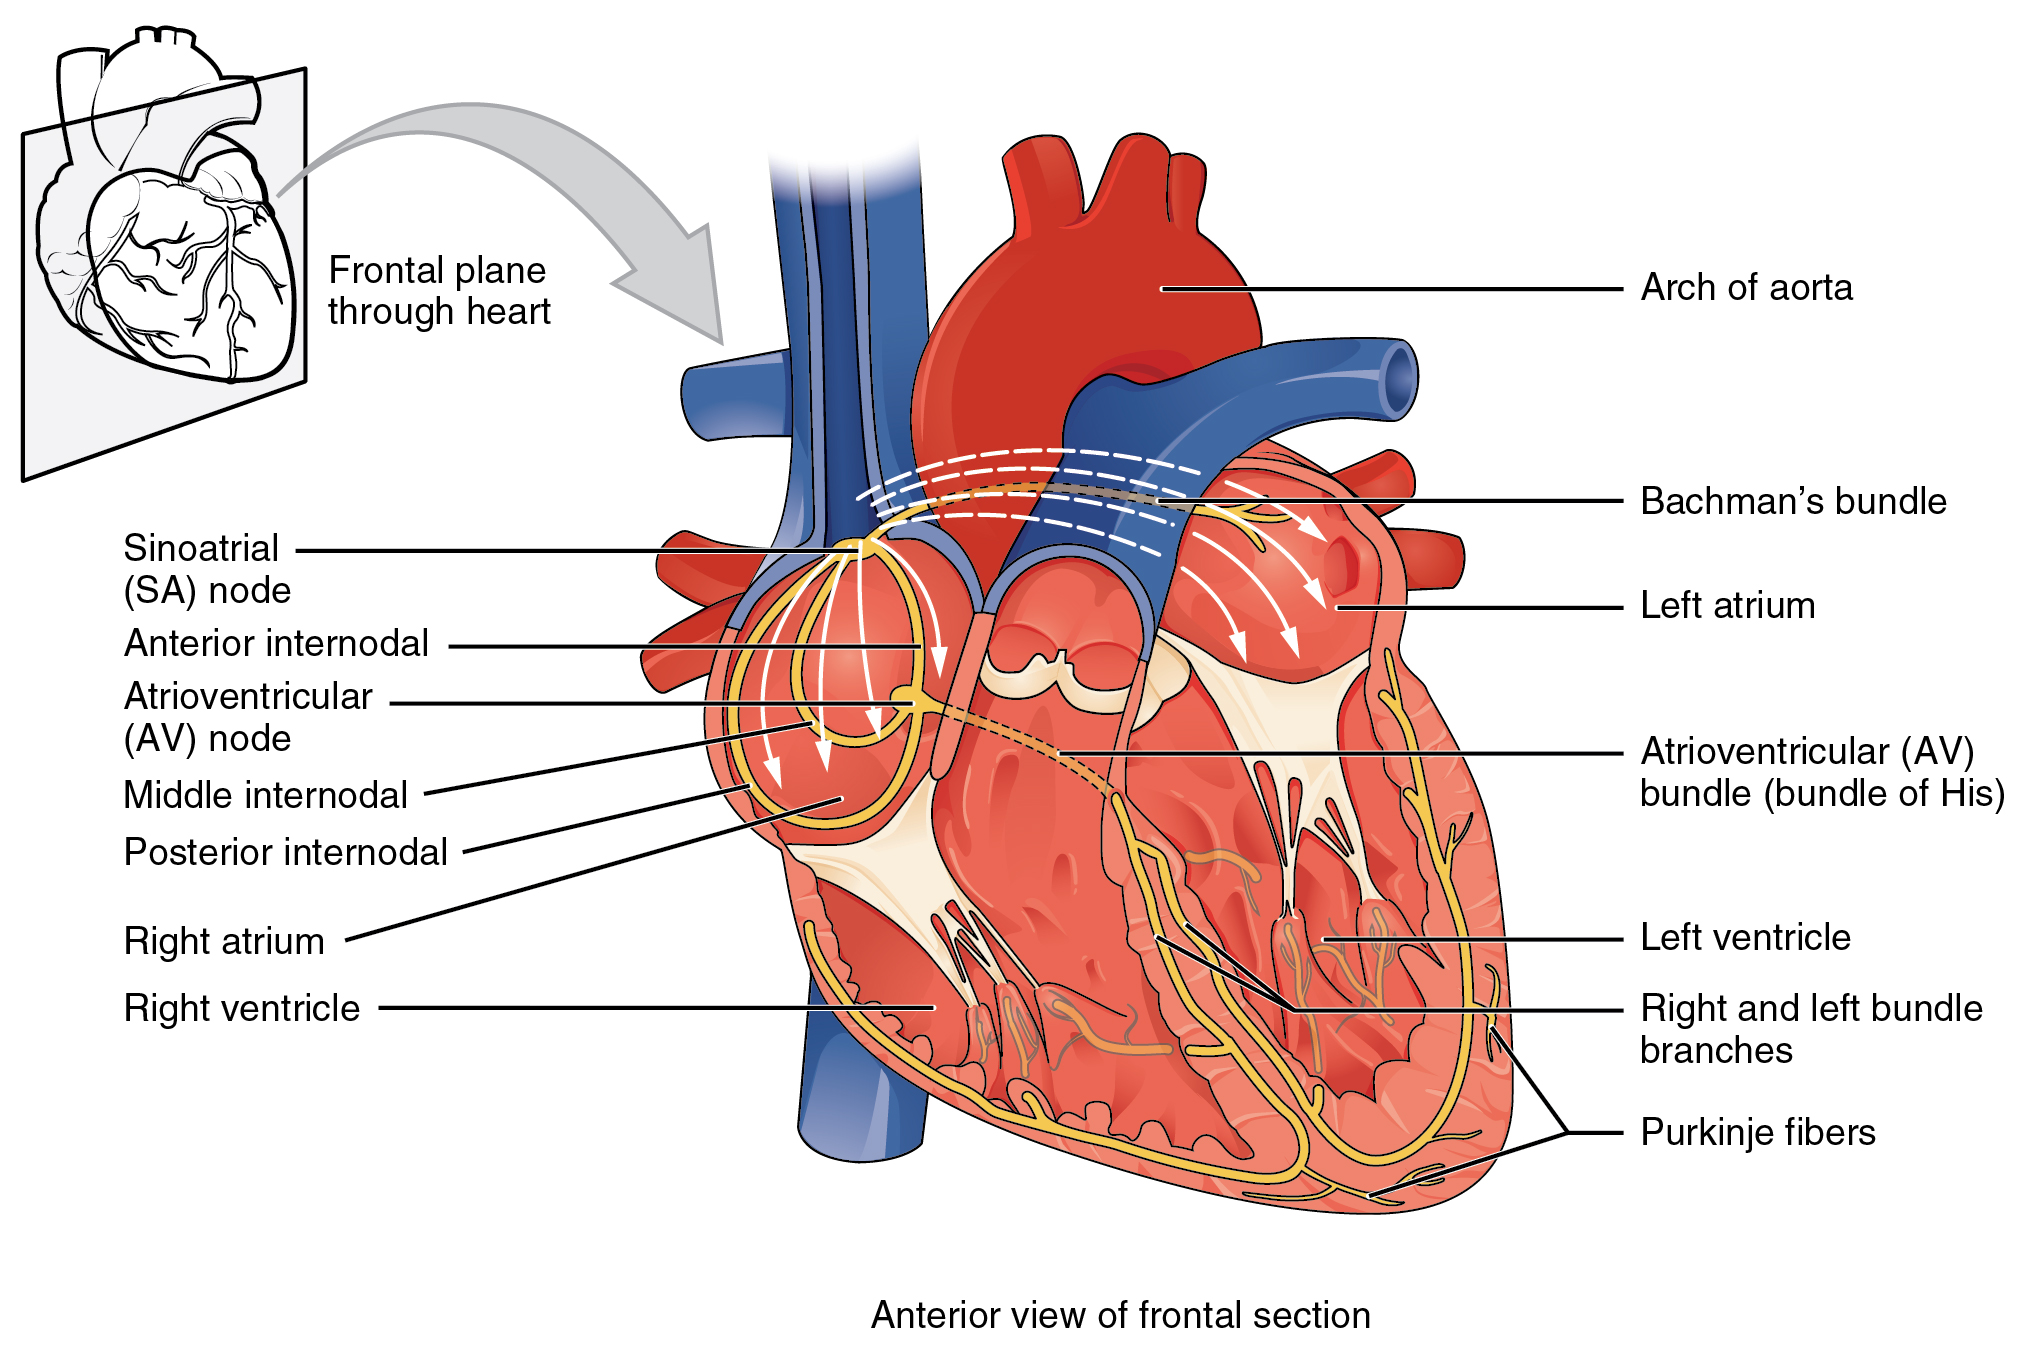
\includegraphics[width=14cm]{figure/conduction-system-of-the-heart.jpeg}
    \caption[Anterior, anatomical view of the conduction system of a human heart.]{Anterior, anatomical view of the conduction system of a human heart. The conducting components of the heart begin with the sinoatrial node and include the internodal pathways, the atrioventricular node, the atrioventricular bundle, the right and left bundle branches, and the Purkinje fibres~\cite{betts-anatomy-and-physiology}.
    Image licensed \texttt{CC BY 4.0} from Betts \emph{et al}~\cite{betts-anatomy-and-physiology} on the OpenStax platform, source: \url{https://openstax.org/books/anatomy-and-physiology/pages/19-2-cardiac-muscle-and-electrical-activity\#fig-ch20_02_02}.}
    \label{fig:heart_conduction_system}
\end{figure}

Figure~\ref{fig:heart_conduction_system} shows an overview of the primary structures relevant to the cardiac conduction cycle.

Starting at rest the sinoatrial node, also known as ``the pacemaker of the heart'', initiates the sinus rhythm action potential which travels across the right and left atria~\cite{betts-anatomy-and-physiology}.
Once the action potential reaches the atrioventricular node, ``there is a delay of approximately 100ms that allows the atria to complete pumping blood before the impluse is transmitted to the atrioventricular bundle''~\cite{betts-anatomy-and-physiology}.
Once the delay finishes, the impluse sweeps across the atrioventricular bundle, right and left bundle branches, and to the Purkinje fibers~\cite{betts-anatomy-and-physiology}.
Ventricular contraction occurs, then the impulse dissipates at the contractile fibers of the ventricle causing the ventricles to repolarize in preparation for the next heartbeat~\cite{betts-anatomy-and-physiology}.

\subsection{Electrocardiogram Tracing}

\begin{figure}[ht]
    \centering
    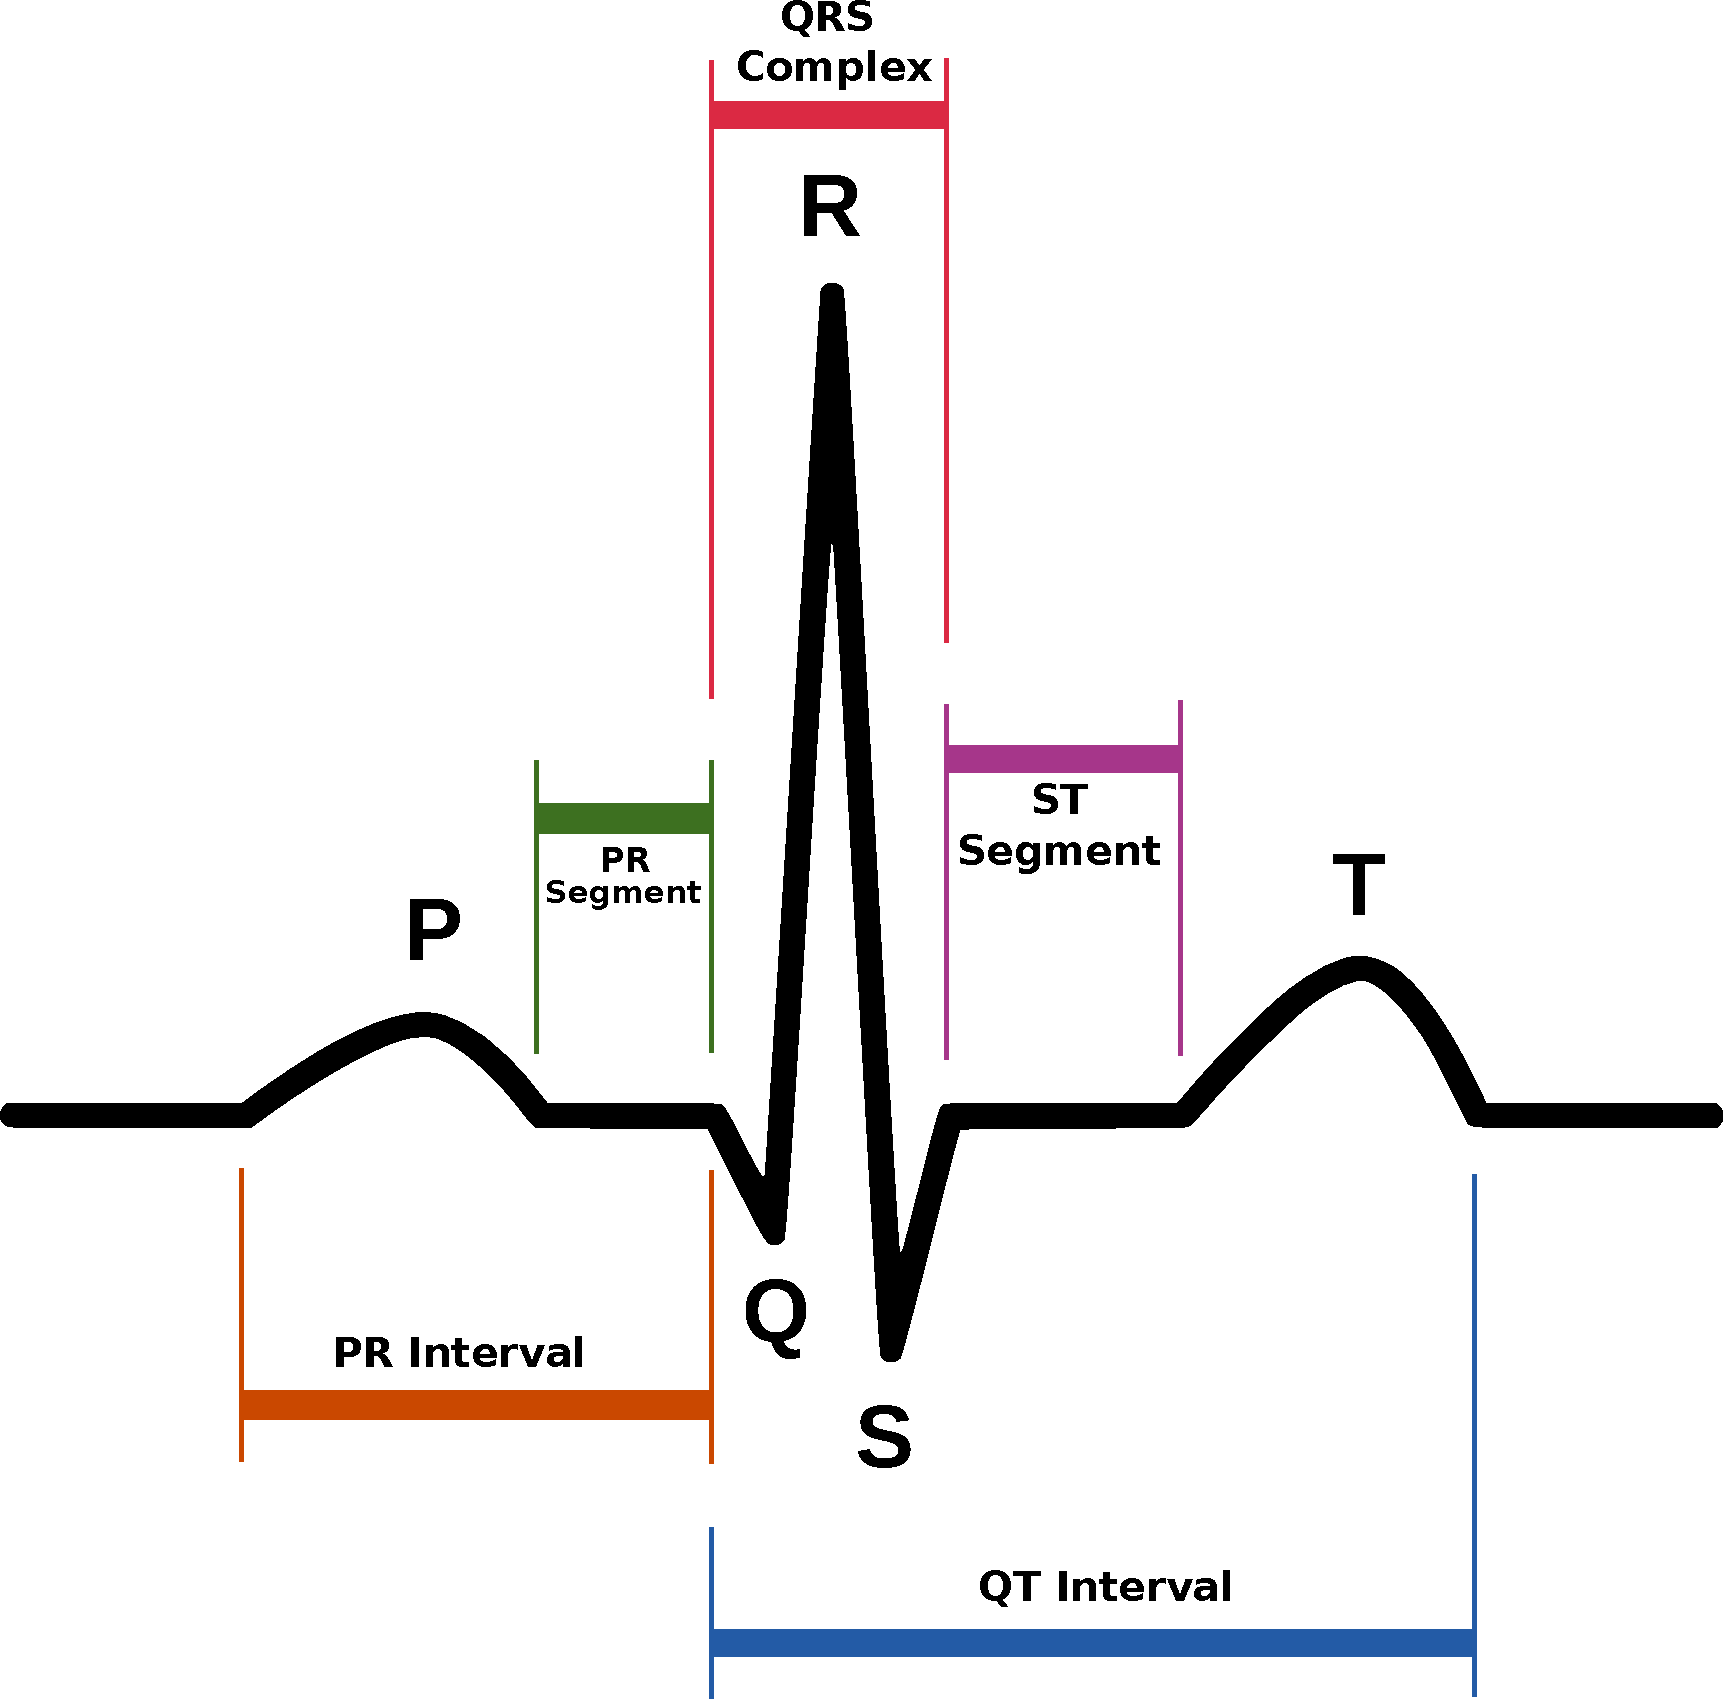
\includegraphics[width=8cm]{figure/PQRST_NormalSinusRhythm.pdf}
    \caption[Normal sinus rhythm \gls{ecg} tracing with PQRST peaks annotated.]{Normal sinus rhythm \gls{ecg} tracing showing the PQRST peaks, the P wave, QRS complex, and T wave along with the PR and QT intervals, plus the PR and ST segments.
    Image belonging to \texttt{public domain} attributed to Anthony Atkielski, source: \url{https://en.wikipedia.org/wiki/Electrocardiography\#/media/File:SinusRhythmLabels.svg}.
    }
    \label{fig:pqrst_nsr}
\end{figure}

Within a typical \gls{ecg}, there are five peaks, labeled PQRST respectively, that define the major components of a heartbeat as shown in Figure~\ref{fig:pqrst_nsr}.
The P wave represents the sinoatrial node initiating an impulse action potential and marks the start of a heartbeat~\cite{betts-anatomy-and-physiology}.
The PR segment, which starts after the P wave and ends before the QRS complex, represents the delay between the atrial contraction and the propagation of the signal through the atrioventricular bundle~\cite{betts-anatomy-and-physiology}.
The QRS complex is the notable large spike in the \gls{ecg}, which represents the electrical impluse traveling through the atrioventricular bundle and bundle branches to the Purkinje fibers~\cite{betts-anatomy-and-physiology}.
The ST segment, starting after the QRS complex and ending before the T wave begins, is the phase of the \gls{ecg} where the actual ventricle contraction occurs~\cite{betts-anatomy-and-physiology}.
After the ventricle contraction completes, the impulse dissipates and allows the ventricle muscles to relax and repolarize, manifesting as the \gls{ecg} T wave~\cite{betts-anatomy-and-physiology}.
A step by step diagram indicating the different \gls{ecg} tracing components and the corresponding cardiac diagram can be found in Figure~\ref{fig:pqrst_heart_conduction_system}.

\begin{figure}[hb]
    \centering
    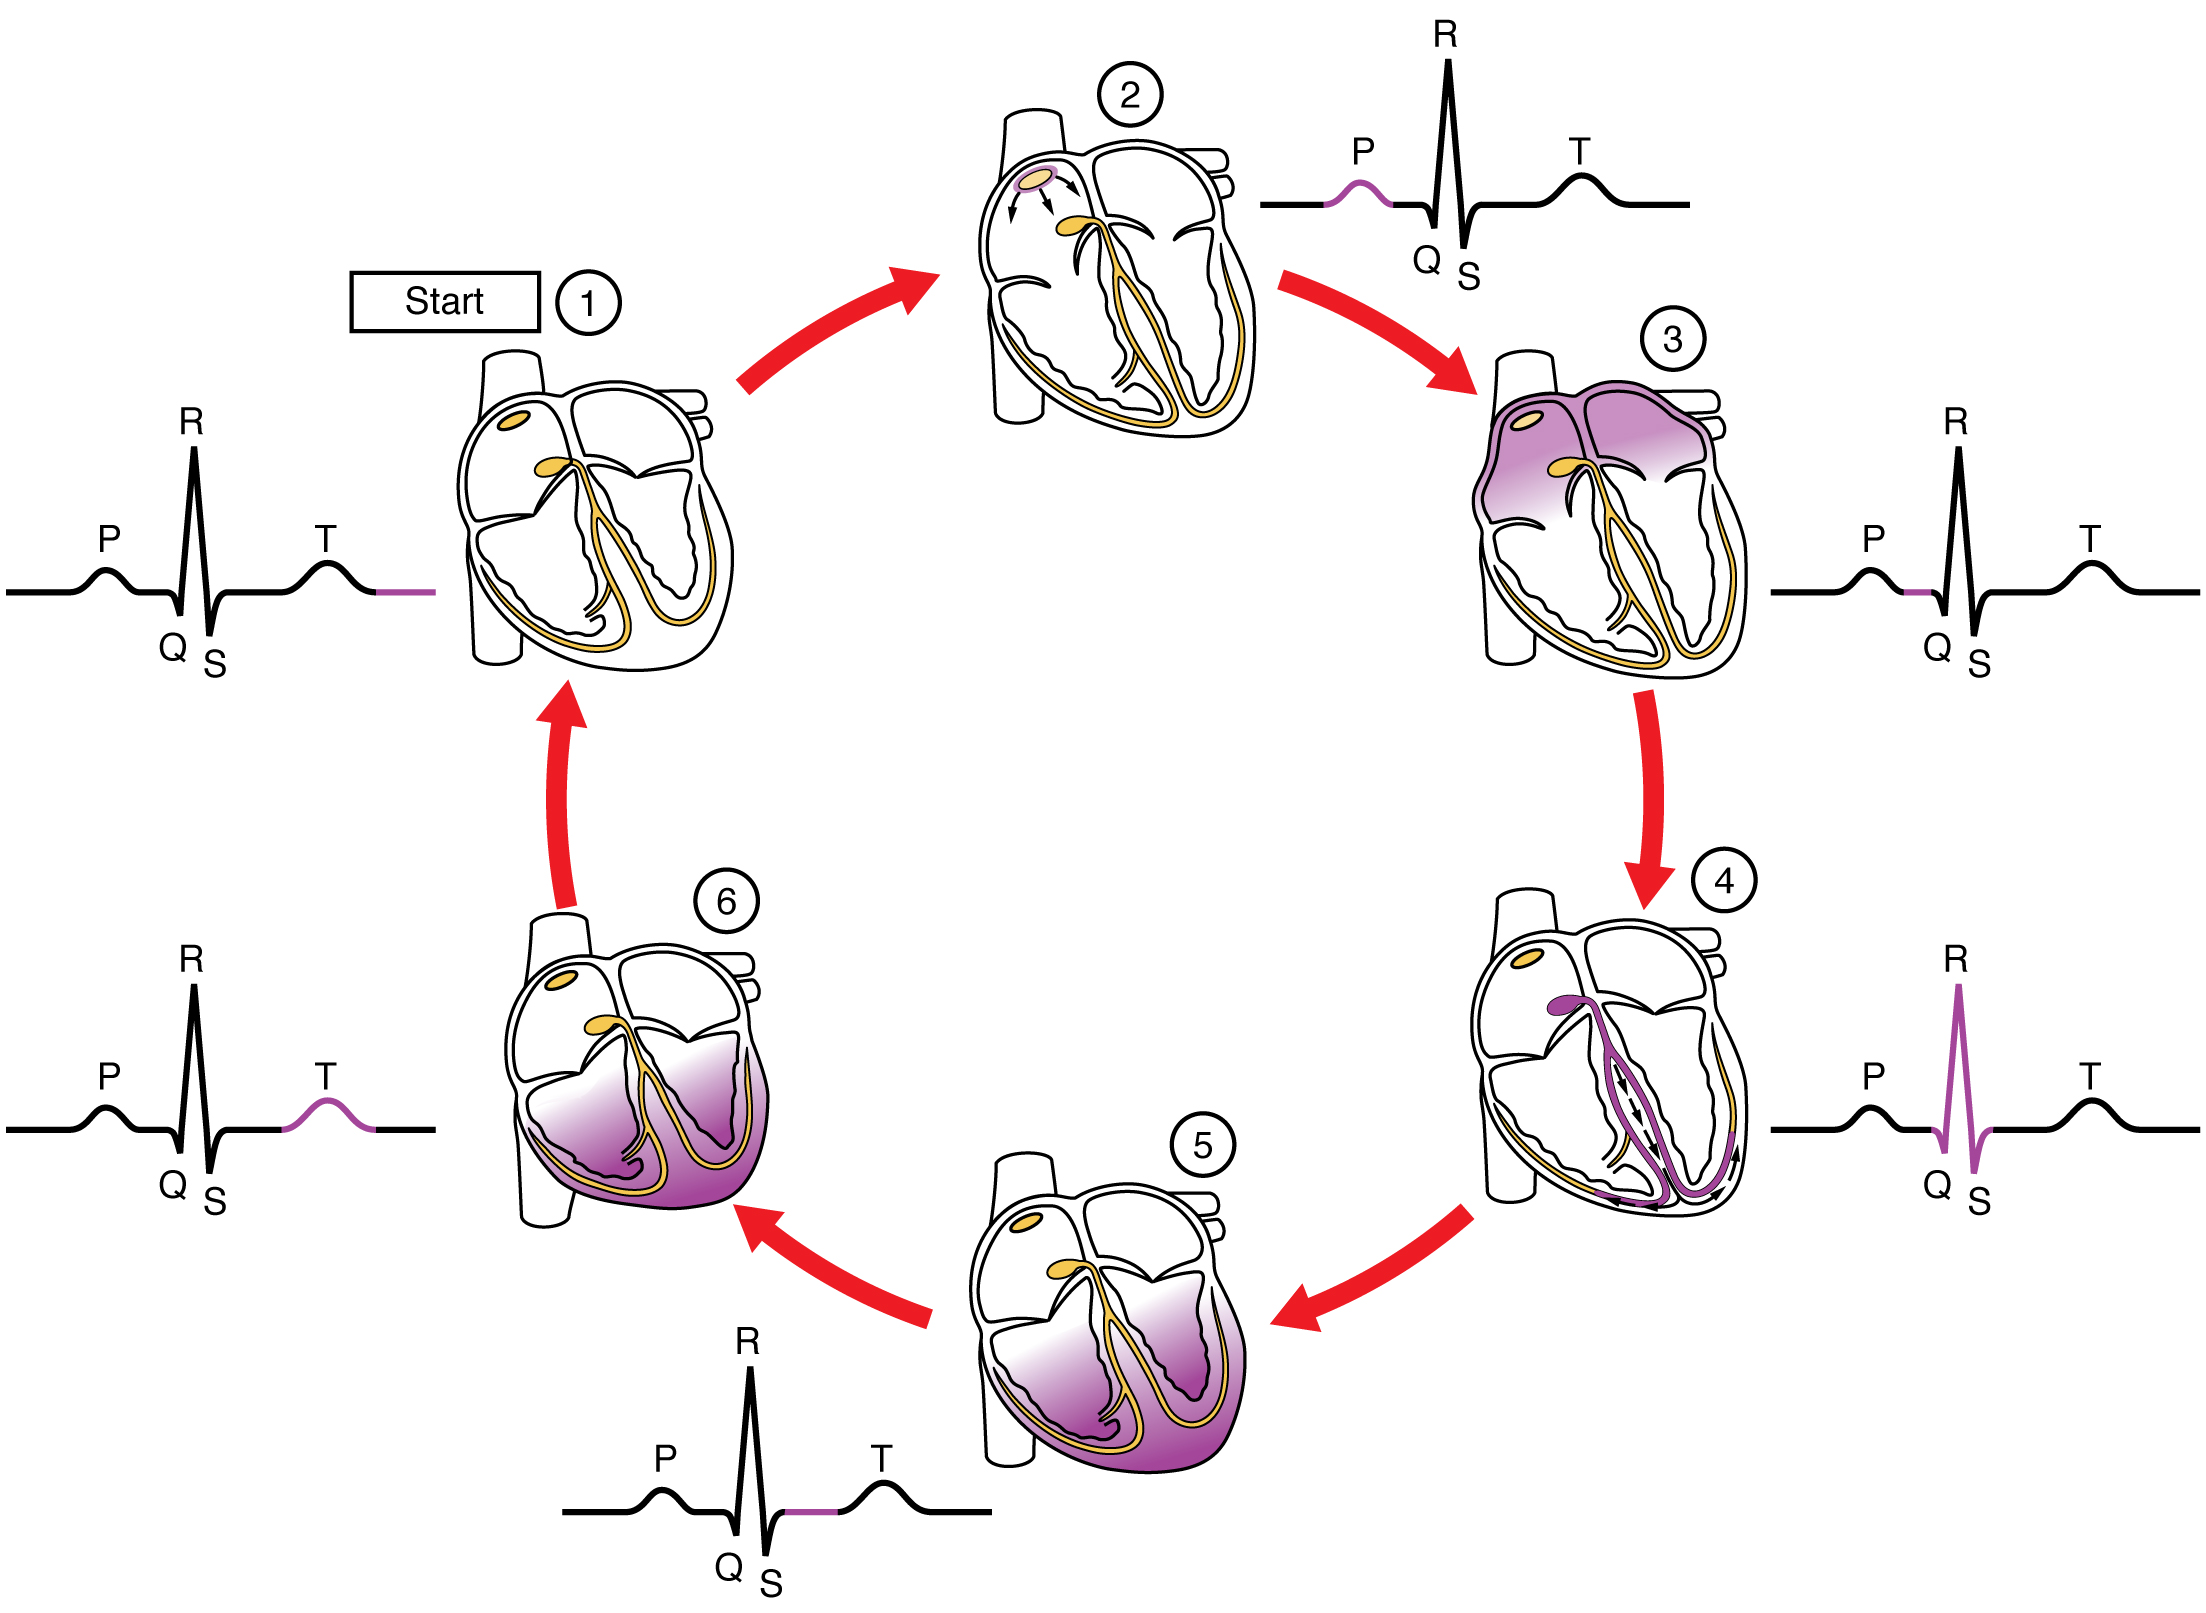
\includegraphics[width=14cm]{figure/pqrst_with_heart_conduction_system.jpeg}
    \caption[Cardiac conduction correlated to ECG tracing waves.]{Cardiac conduction correlated to ECG tracing waves~\cite{betts-anatomy-and-physiology}.
    1. The conduction system of the heart is currently at rest, with the ventricles repolarized.
    2. The sinoatrial node begins an action potential which permeates across the atria, causing the \gls{ecg} P wave formation.
    3. A 100ms delay in the impulse occurs which allows the atria to complete pumping blood, showing as the PR segment in the \gls{ecg}.
    4. The impulse proceeds through the atrioventricular bundle and bundle branches to the Purkinje fibers, appearing as the QRS complex in the \gls{ecg}.
    5. The contractile fibers of the ventricles are stimulated by the impulse, causing the ventricles to contract and appears as the ST-segment in the \gls{ecg}.
    6. The impulse dissipates and the ventricular muscles relax, causing the \gls{ecg} T wave formation.
    Image licensed \texttt{CC BY 4.0} from Betts \emph{et al}~\cite{betts-anatomy-and-physiology} on the OpenStax platform, source: \url{https://openstax.org/books/anatomy-and-physiology/pages/19-2-cardiac-muscle-and-electrical-activity\#fig-ch20_02_08}.}
    \label{fig:pqrst_heart_conduction_system}
\end{figure}

\subsection{Electrode Placement and Cardiac Axis}

\begin{figure}[ht]
    \centering
    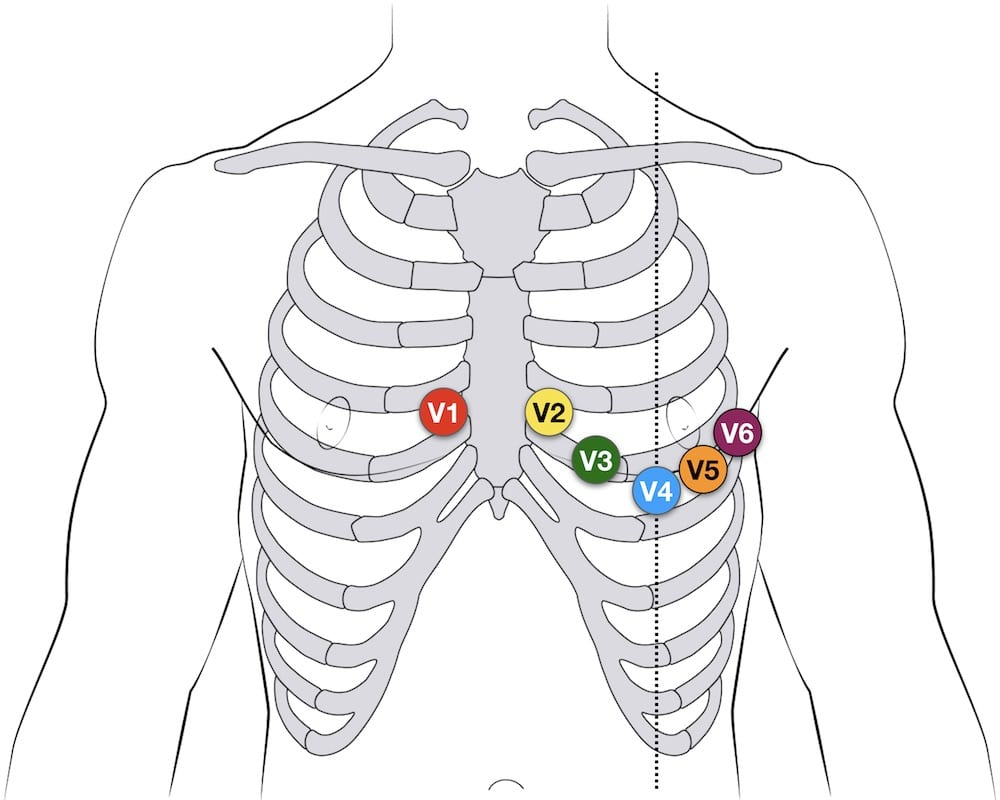
\includegraphics[width=12cm]{figure/12-lead-ECG-lead-placement.jpg}
    \caption[Placement of 12-lead ECG for precordial electrodes V1-V6.]{Placement of 12-lead ECG for precordial electrodes V1-V6~\cite{ecg-lead-positioning}. V1 is located in the 4th intercostal space (ICS) on the right margin of the sternum. V2 is placed at the 4th ICS on the left margin of the sternum. V3 is placed midway between V2 and V4. V4 is placed on the 5th ICS mid-clavicular line. V5 is placed on the anterior axillary line at the same level as V4 (5th ICS). V6 is placed on the mid-axillary line at the same level as V4 (5th ICS).
    Image licensed \texttt{CC BY-NC-SA 4.0} from Mike Cadogan~\cite{ecg-lead-positioning} on the Life In The Fast Lane platform, source: \url{https://litfl.com/ecg-lead-positioning/}.}
    \label{fig:12-lead-ecg-placement}
\end{figure}

The 12-lead \gls{ecg} is derived from 10 electrodes placed on the surface of the skin~\cite{ecg-lead-positioning}.
The positioning of the leads is critical to ensure that the proper traces are recorded.
See Figure~\ref{fig:12-lead-ecg-placement} for a guide to placing the 6 precordial (front of the heart) leads V1 to V6.
The remaining four leads are extremity or limb electrodes: Right Arm (RA) should be placed anywhere between the right shoulder and right elbow; Right Leg (RL) should be placed below the right torso and above the right ankle; Left Arm (LA) should be placed between the left shoulder and left elbow; and Left Leg (LL) should be placed below the left torso and above the left ankle~\cite{ecg-lead-positioning}.

When reading a 12-lead \gls{ecg}, the leads I, II, II, aVR, aVL, and aVF are derived from the limb leads~\cite{goldberger_simple_1942}.
\begin{equation}
    V_W = \dfrac{1}{3}(RA + LA + LL) \label{eq:wilson_central_terminal}
\end{equation}
Equation~\ref{eq:wilson_central_terminal} shows a common virtual electrode, known as the Wilson's central terminal, defined by averaging three of the limb leads (RA, LA, LL) together~\cite{goldberger_simple_1942}.
\begin{equation}
    I = LA - RA \label{eq:lead_I}
\end{equation}
\begin{equation}
    II = LL - RA \label{eq:lead_II}
\end{equation}
\begin{equation}
    III = LL - LA \label{eq:lead_III}
\end{equation}
The unused limb lead RL does not show up in the \gls{ecg} readings and is considered a neutral grounding lead for minimizing artifacts~\cite{ecg-lead-positioning}.
See Equation~\ref{eq:lead_I} for lead I, Equation~\ref{eq:lead_II} for lead II, and Equation~\ref{eq:lead_III} for lead III~\cite{goldberger_simple_1942}.
\begin{equation}
    aVR = \dfrac{3}{2}(RA - V_W) = RA - \dfrac{1}{2}(LA + LL) \label{eq:lead_aVR}
\end{equation}
\begin{equation}
    aVL = \dfrac{3}{2}(LA - V_W) = LA - \dfrac{1}{2}(RA + LL) \label{eq:lead_aVL}
\end{equation}
\begin{equation}
    aVF = \dfrac{3}{2}(LL - V_W) = LL - \dfrac{1}{2}(RA + LA) \label{eq:lead_aVF}
\end{equation}
The augmented limb leads aVR, aVL, and aVF are derived from the same three electrodes as leads I, II, and III but rely on Wilson's central terminal as their negative pole.
See Equation~\ref{eq:lead_aVR} for lead aVR, Equation~\ref{eq:lead_aVL} for lead aVL, and Equation~\ref{eq:lead_aVF} for lead aVF~\cite{goldberger_simple_1942}.
The remaining precordial leads V1 to V6 shown in the ECG are the directly measured signals from the electrodes.

An \gls{ecg}'s cardiac axis refers to the average direction of the wave of ventricular depolarization measured from the reference point of lead I on a standard 12-lead \gls{ecg}~\cite{meek_introduction_2002}.
One simple estimation of the cardiac axis is done by inspecting the magnitude of the R-peaks on leads I, II, and III~\cite{ecg-left-axis-deviation}.
In a normal \gls{ecg}, leads I, II are positive while lead III may be positive or negative.
There is right axis deviation if lead I is negative and lead III is positive (lead II may be positive or negative).
Left axis deviation exists if lead I is positive while leads II and III are negative.

\begin{figure}
    \centering
    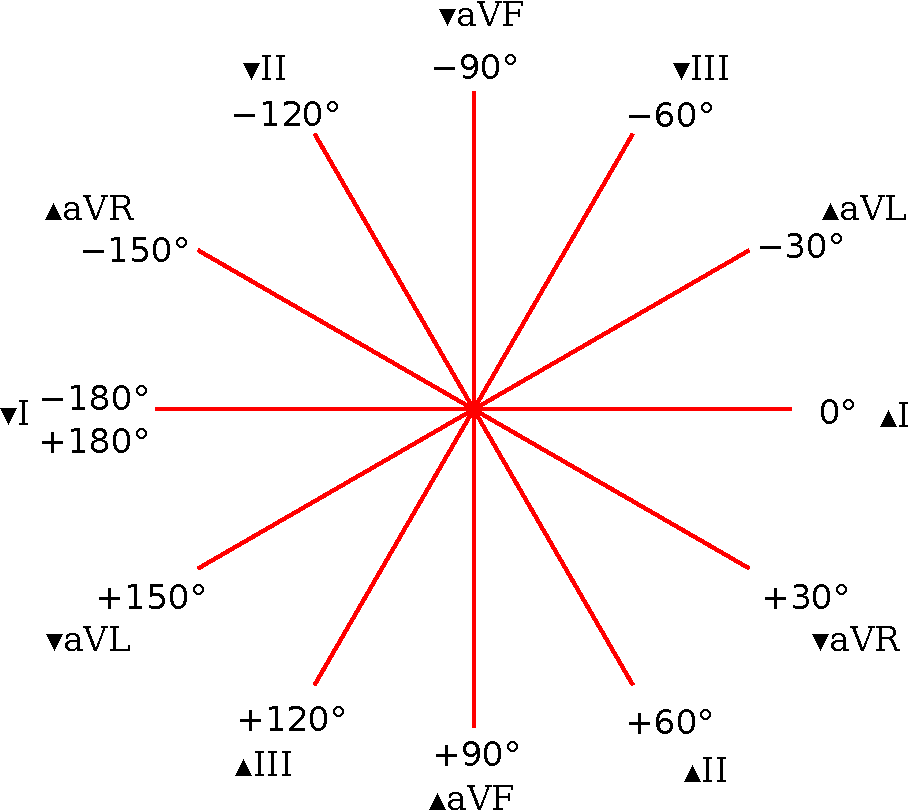
\includegraphics[width=10cm]{figure/Hexaxial_reference_system.pdf}
    \caption[Hexaxial (Cabrera) system for determining cardiac axis. Six frontal planes are viewed in the sequence aVL, I, aVR, II, aVF, and III.]{Hexaxial (Cabrera) system for determining cardiac axis~\cite{valentinuni1970properties}. Six frontal planes are viewed in the sequence aVL, I, aVR, II, aVF, and III. Within an ECG record, the lead with the maximum QRS peak amplitude change, positive or negative, is used as the estimate for the cardiac electrical axis.
    Image belonging to \texttt{public domain} from Wikipedia users MoodyGroove and Mysid, source: \url{https://commons.wikimedia.org/w/index.php?curid=2635587}.
    }
    \label{fig:hexaxial_reference}
\end{figure}

Alternatively, the Cabrera system or hexaxial reference system, can be used to logically derive the heart's electrical axis~\cite{lam_classical_2015, valentinuni1970properties}.
By viewing the six frontal planes in the sequence aVL, I, aVR, II, aVF, and III, we check the maximal amplitude of the ECG vector (positive or negative) and use it to derive the cardiac electrical axis.
Figure~\ref{fig:hexaxial_reference} shows the hexaxial reference system and the mapping to the six derived limb leads.
A normal axis is a value between $-30\degree$ to $90\degree$, left axis deviation is between $-30\degree$ to $-90$, right axis deviation is between $90\degree$ to $180\degree$.
Values that exceed the defined ranges are classified as extreme axis deviations.

\section{PhysioNet/CinC 2020 Challenge Overview}

This chapter summarizes the task of multi-label, multi-class classification of \gls{ecg}s as proposed by Perez Alday \emph{et al.}~\cite{physionet_challenge_2020} in the \emph{PhysioNet/CinC 2020 Challenge}.

\subsection{Public Dataset}
The challenge provided a public collection of 43,101 labelled \gls{ecg} records for training.
These public records were sourced from multiple locations, including:

\begin{enumerate}
    \item The China Physiological Signal Challenge (\textbf{CPSC}) 2018~\cite{liu_open_2018} corpus of data, containing 10,330 recordings.
    \item The St. Petersburg Institute of Cardiological Technics (\textbf{INCART}) database of 12-lead arrhythmias~\cite{tihonenko2008st}, containing 74 recordings.
    \item The Physikalisch Technische Bundesanstalt (PTB) contributed datasets \textbf{PTB} Diagnostic \gls{ecg} Database~\cite{NutzungderEKGSignaldatenbankCARDIODATderPTBberdasInternet} and the more recent \textbf{PTB-XL} database~\cite{wagner_ptb-xl_2020}, containing a combined total of 22,353 records.
    \item The Georgia 12-lead \gls{ecg} Challenge (\textbf{G12EC}) database, containing 10,344 records.
\end{enumerate}

A separate hold-out set of \gls{ecg} records is sourced from an undisclosed organization containing patients geographically distinct from the publicly available data.
This hold-out set of data is used for the official challenge test phase only and is not available to researchers.
In my analysis, I do not make any distinction between the different \gls{ecg} source locations and combine all of the records into a single repository.
Two \gls{ecg} records (\texttt{Training\_2/Q0400}, \texttt{Training\_2/Q2961} from the CPSC2018 tranche of signals) containing no activity on any leads are excluded from analysis.

\begin{figure}[ht]
    \centering
    \textbf{Count of Patient Age by Sex}\par\medskip
    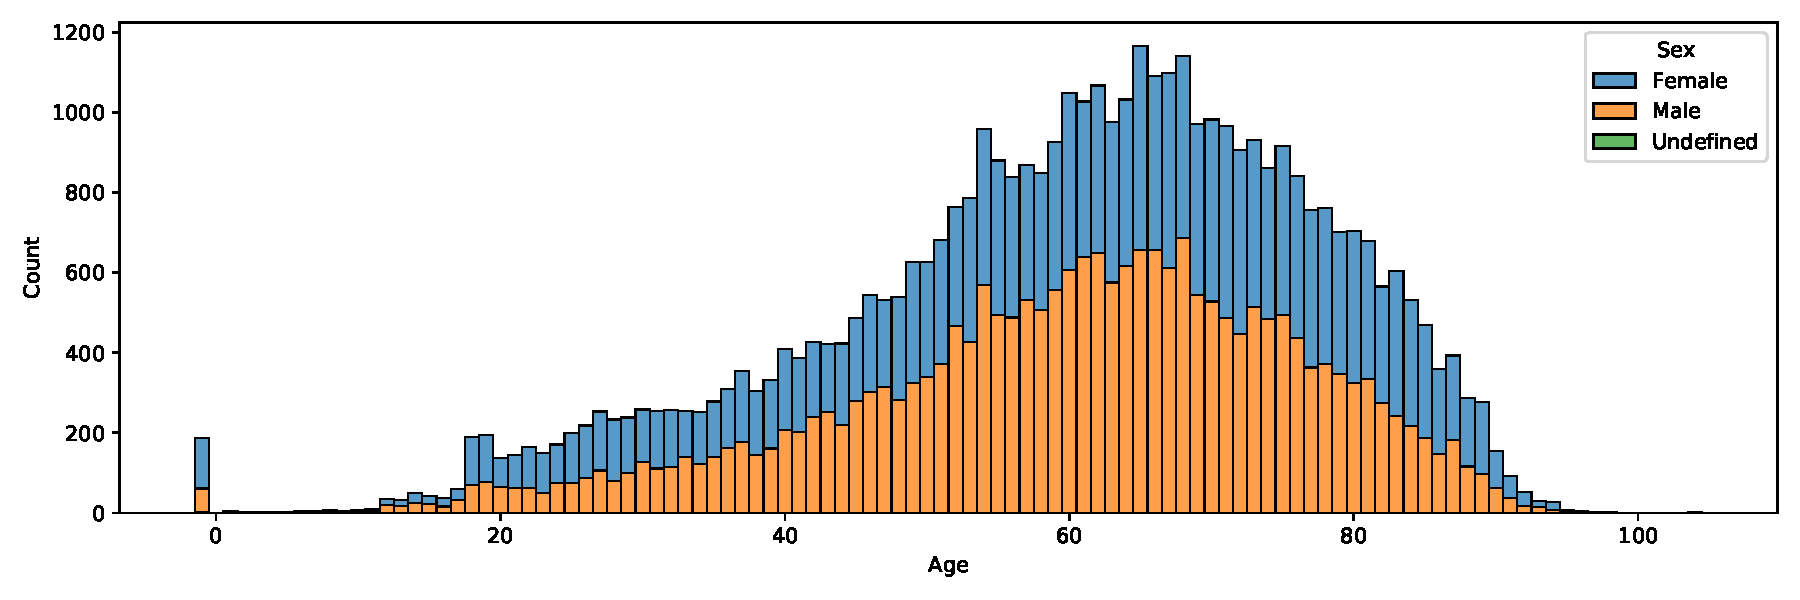
\includegraphics[width=14cm]{figure/age_sex_hist.pdf}
    \caption[Age and sex distribution of the PhysioNet/CinC 2020 public electrocardiogram dataset.]{Age and sex distribution of the PhysioNet/CinC 2020 public electrocardiogram dataset.
    Records with age $<0$ indicate that age is not provided for the given record. The only record that is missing the biological sex metadata is also missing the age metadata.}
    \label{fig:age_sex_hist}
\end{figure}

Each \gls{ecg} record also contains additional metadata in the form of the patient age and biological sex.
There are 187 records that contain an undefined age.
Of the remaining records, the mean patient age is 60.3.
The \gls{ecg} records contained primarily male and female sex, with 46.9\% of the patients in the dataset as female, 53.1\% of the patients as male, and one record that did not have the sex metadata specified.
A histogram showcasing the distribution of the age and sex in our dataset can be found in Figure~\ref{fig:age_sex_hist}.

\subsection{Diagnosed Labels}

\begin{table}[t]
    \caption{\label{tab:labels_snomed_ct} Evaluated SNOMED CT codes with definition, count and percentage in dataset.}
    \vspace{2 mm}
    \centerline{\begin{tabular}{@{}ll@{}l@{}r@{}}
    SNOMED & Abbr. & Diagnosis & Count (\%) \\ \hline
    270492004 & IAVB & 1st degree av block & 2394 (5.6\%) \\
    164889003 & AF & atrial fibrillation & 3475 (8.0\%) \\
    164890007 & AFL & atrial flutter & 314 (0.7\%) \\
    426627000 & Brady & bradycardia & 288 (0.7\%) \\
    713427006 & CRBBB & complete right bundle branch block & 683 (1.6\%) \\
    713426002 & IRBBB & incomplete right bundle branch block & 1611 (3.7\%) \\
    445118002 & LAnFB & left anterior fascicular block & 1806 (4.2\%) \\
    39732003 & LAD & left axis deviation & 6086 (14.1\%)  \\
    164909002 & LBBB & left bundle branch block & 1041 (2.4\%) \\
    251146004 & LQRSV & low QRS voltages & 556 (1.3\%) \\
    698252002 & {{NSIVCB }} & nonspecific intraventricular conduction & 997 (2.3\%) \\
    10370003 & PR & pacing rhythm & 299 (0.7\%) \\
    284470004 & PAC & premature atrial contraction & 1729 (4.0\%) \\
    427172004 & PVC & premature ventricular contractions & 188 (0.4\%) \\
    164947007 & LPR & prolonged PR interval & 340 (0.7\%) \\
    111975006 & LQT & prolonged QT interval & 1513 (3.5\%) \\
    164917005 & QAb & Q wave abnormal & 1013 (2.4\%) \\
    47665007 & RAD & right axis deviation & 427 (1.0\%) \\
    59118001 & RBBB & right bundle branch block & 2402 (5.6\%) \\
    427393009 & SA & sinus arrhythmia & 1240 (2.9\%) \\
    426177001 & SB & sinus bradycardia & 2359 (5.5\%) \\
    426783006 & SNR & sinus rhythm & 20846 (48.4\%)  \\
    427084000 & STach & sinus tachycardia & 2402 (5.6\%) \\
    63593006 & SVPB & supraventricular premature beats & 215 (0.5\%) \\
    164934002 & TAb & T wave abnormal & 4673 (10.8\%)  \\
    59931005 & TInv & T wave inversion & 1112 (2.6\%) \\
    17338001 & VPB & ventricular premature beats & 365 (0.8\%) \\ \hline
    \end{tabular}}
\end{table}

Each record in our available dataset is labelled with at least one numerical \gls{snomed} clinical term (CT).
For the purpose of the challenge, a subset of 27 codes/labels have been selected for classification.
All other codes are ignored in this study.
Please refer to Table~\ref{tab:labels_snomed_ct} for the labels, abbreviations, counts, and proportion within the dataset.



\begin{description}
    \begin{figure}[H]
        \centering
        \makebox[\textwidth][c]{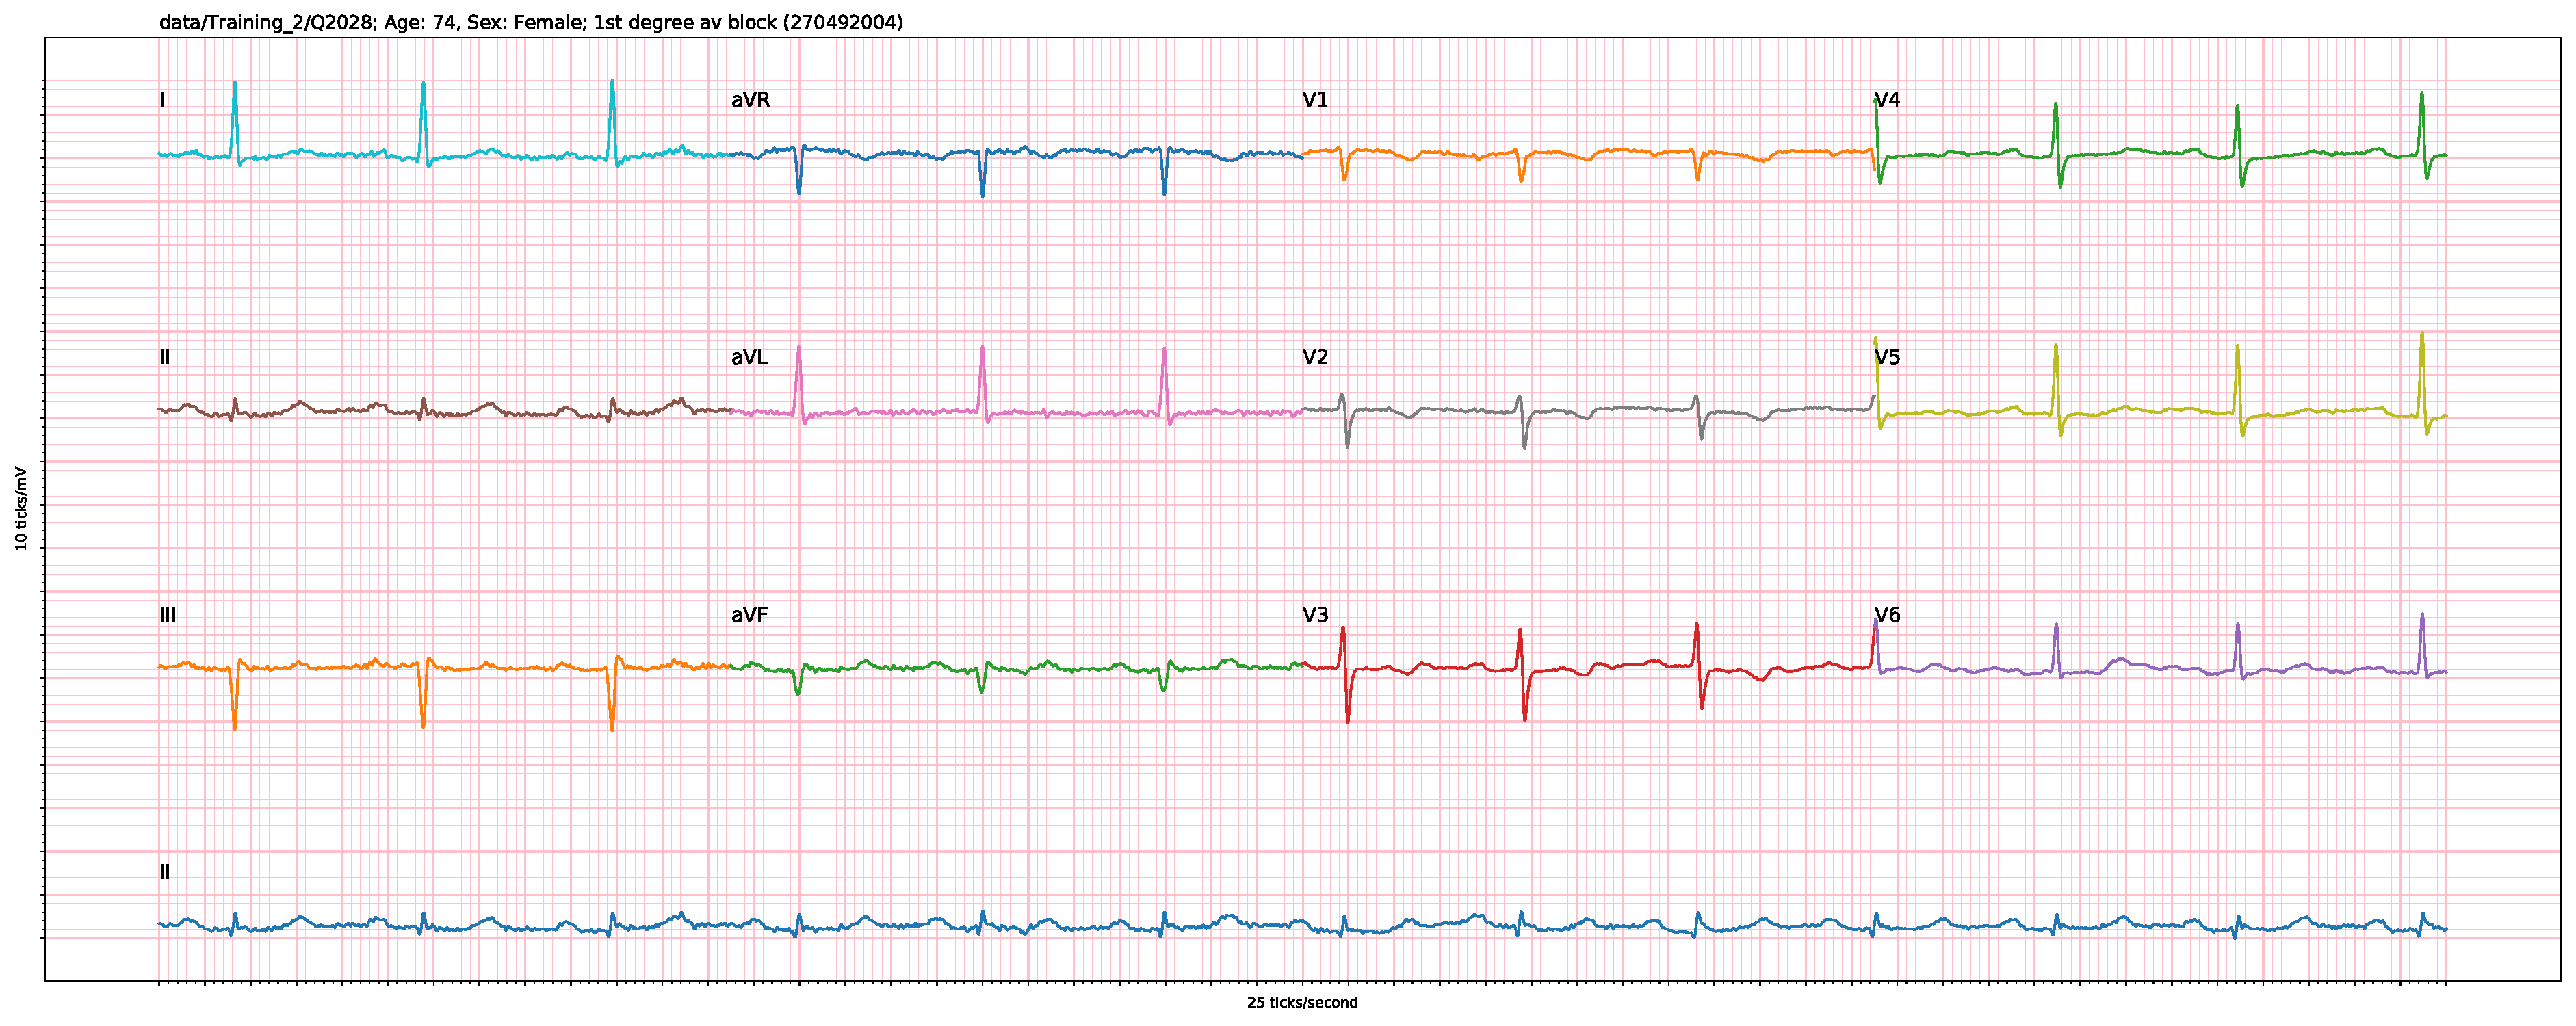
\includegraphics[width=1.2\textwidth]{figure/IAVB/full_0_1951.pdf}}
        \caption{Instance of \gls{ecg} record with 1st degree av block. Long PR interval greater than 200ms is observed.}
        \label{fig:full_IAVB}
    \end{figure}
    \item[\gls{iavb}] This is when there is an abnormally long delay between the electrical impulse from the atria, through the ventricular node, to the ventricles. On the \gls{ecg}, this is detected by the presence of a PR interval longer than 200ms~\cite{carroz_pseudo-pacemaker_2010} or by the existence of a notched (bimodal) P-wave in leads I, II, III, and aVF~\cite{bayes_de_luna_diagnosis_2017}. See Figure~\ref{fig:full_IAVB} for an example of an \gls{ecg} record containing this ailment.
    
    \begin{figure}[H]
        \centering
        \makebox[\textwidth][c]{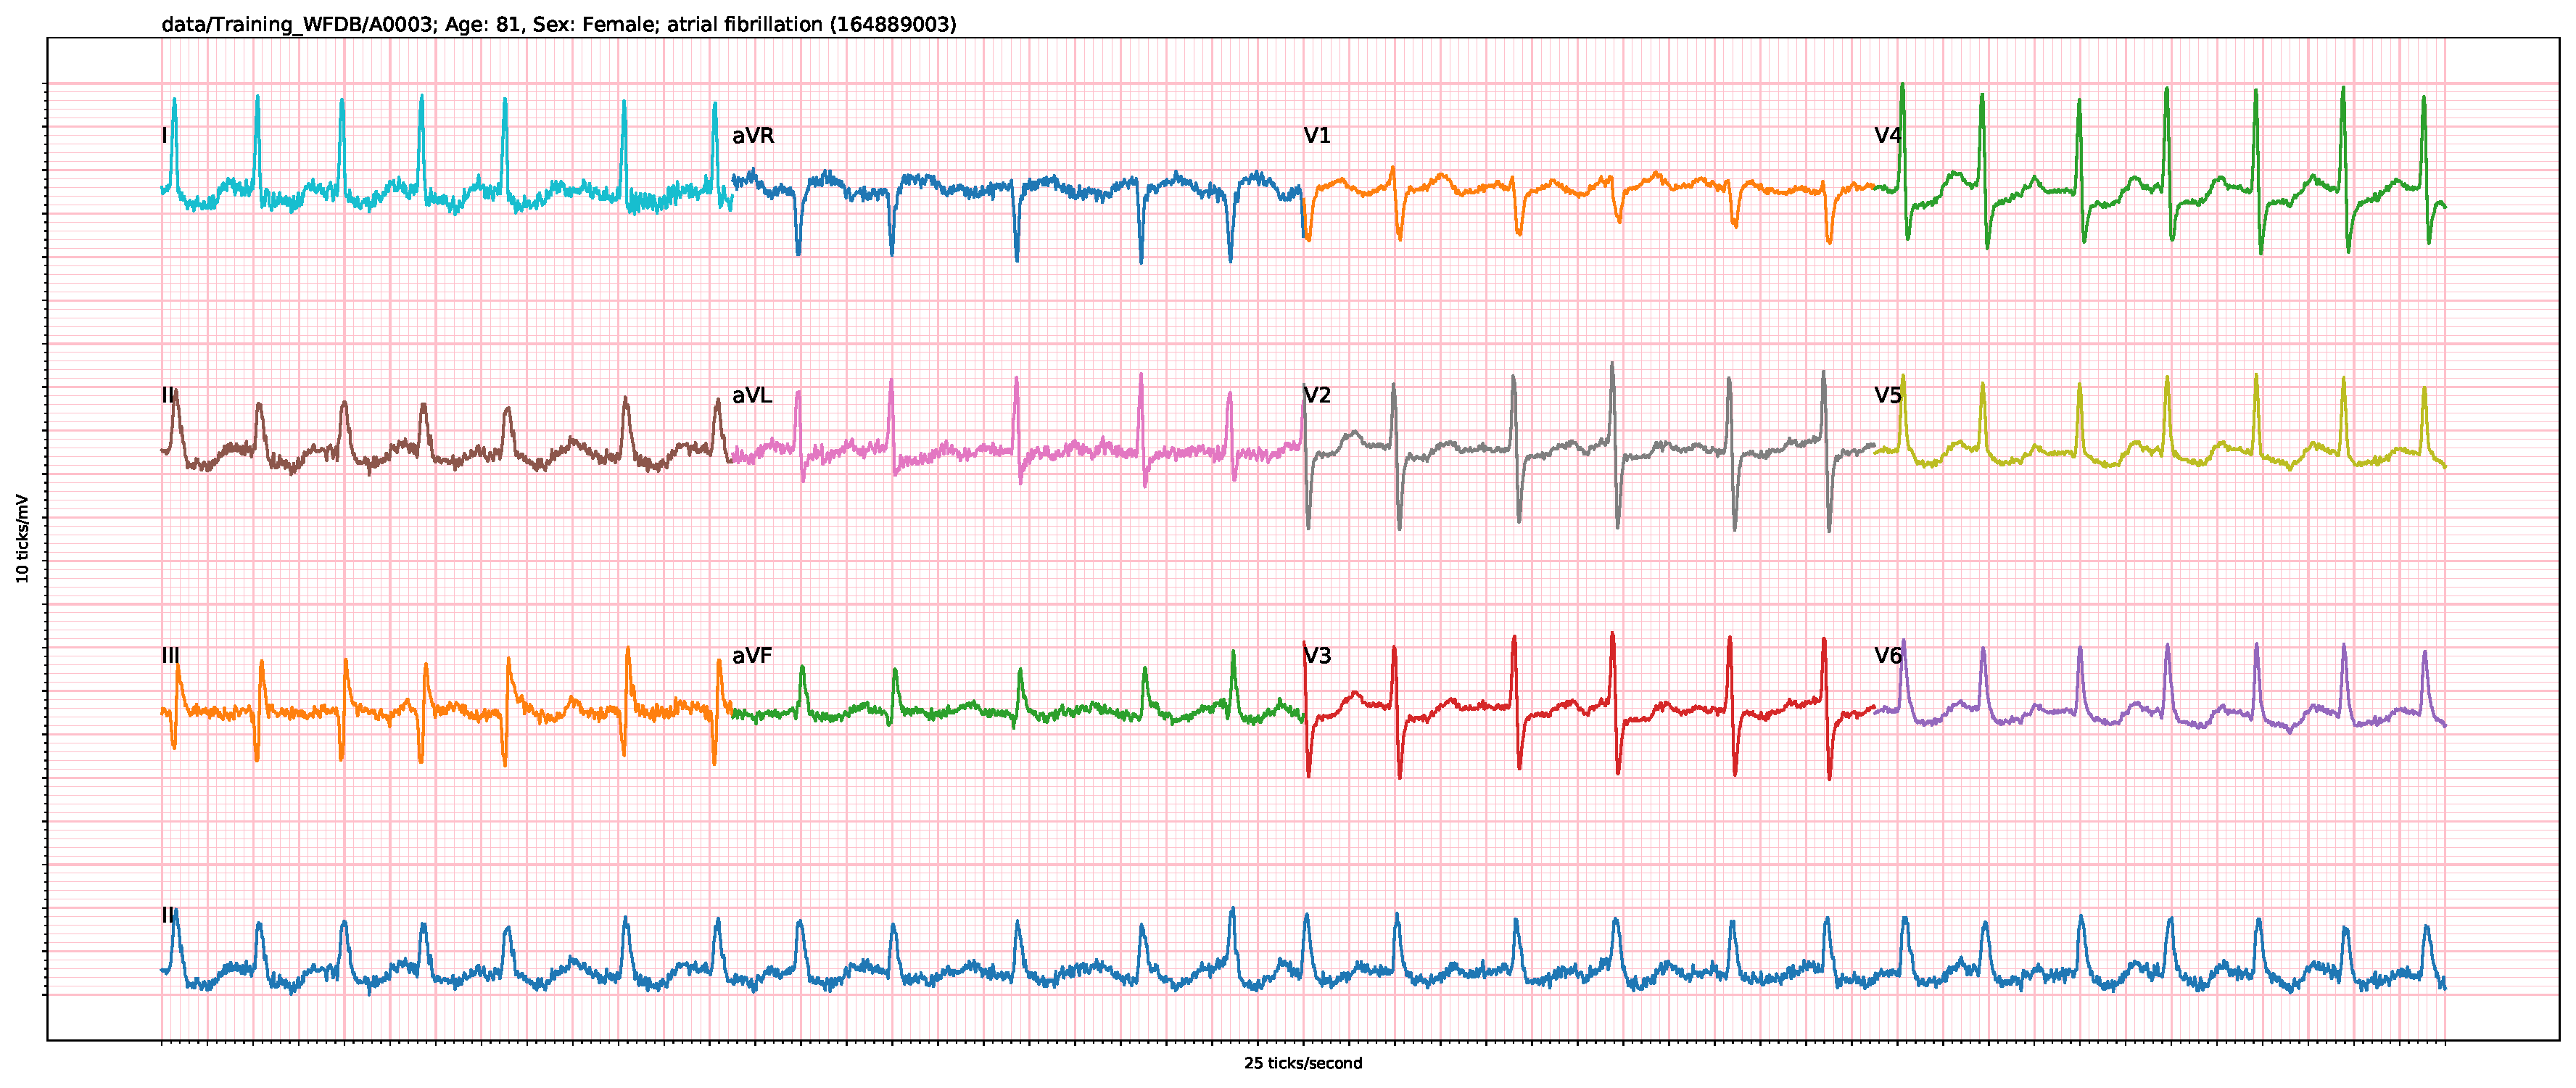
\includegraphics[width=1.2\textwidth]{figure/AF/full_0_3453.pdf}}
        \caption{Instance of 12-lead \gls{ecg} with atrial fibrillation. Irregular, fibrillatory p-waves found in all leads.}
        \label{fig:full_AF}
    \end{figure}
    \item[\gls{af}] The manifestation of \gls{af} may take on multiple forms, ranging from the absence of P waves, irregular heartbeat rhythm, or fibrillatory (rapid, fluttering) P-waves~\cite{podrid2001cardiac,afib-ecg}. Figure~\ref{fig:full_AF} shows an \gls{ecg} instance with this disorder.

    \begin{figure}[H]
        \centering
        \makebox[\textwidth][c]{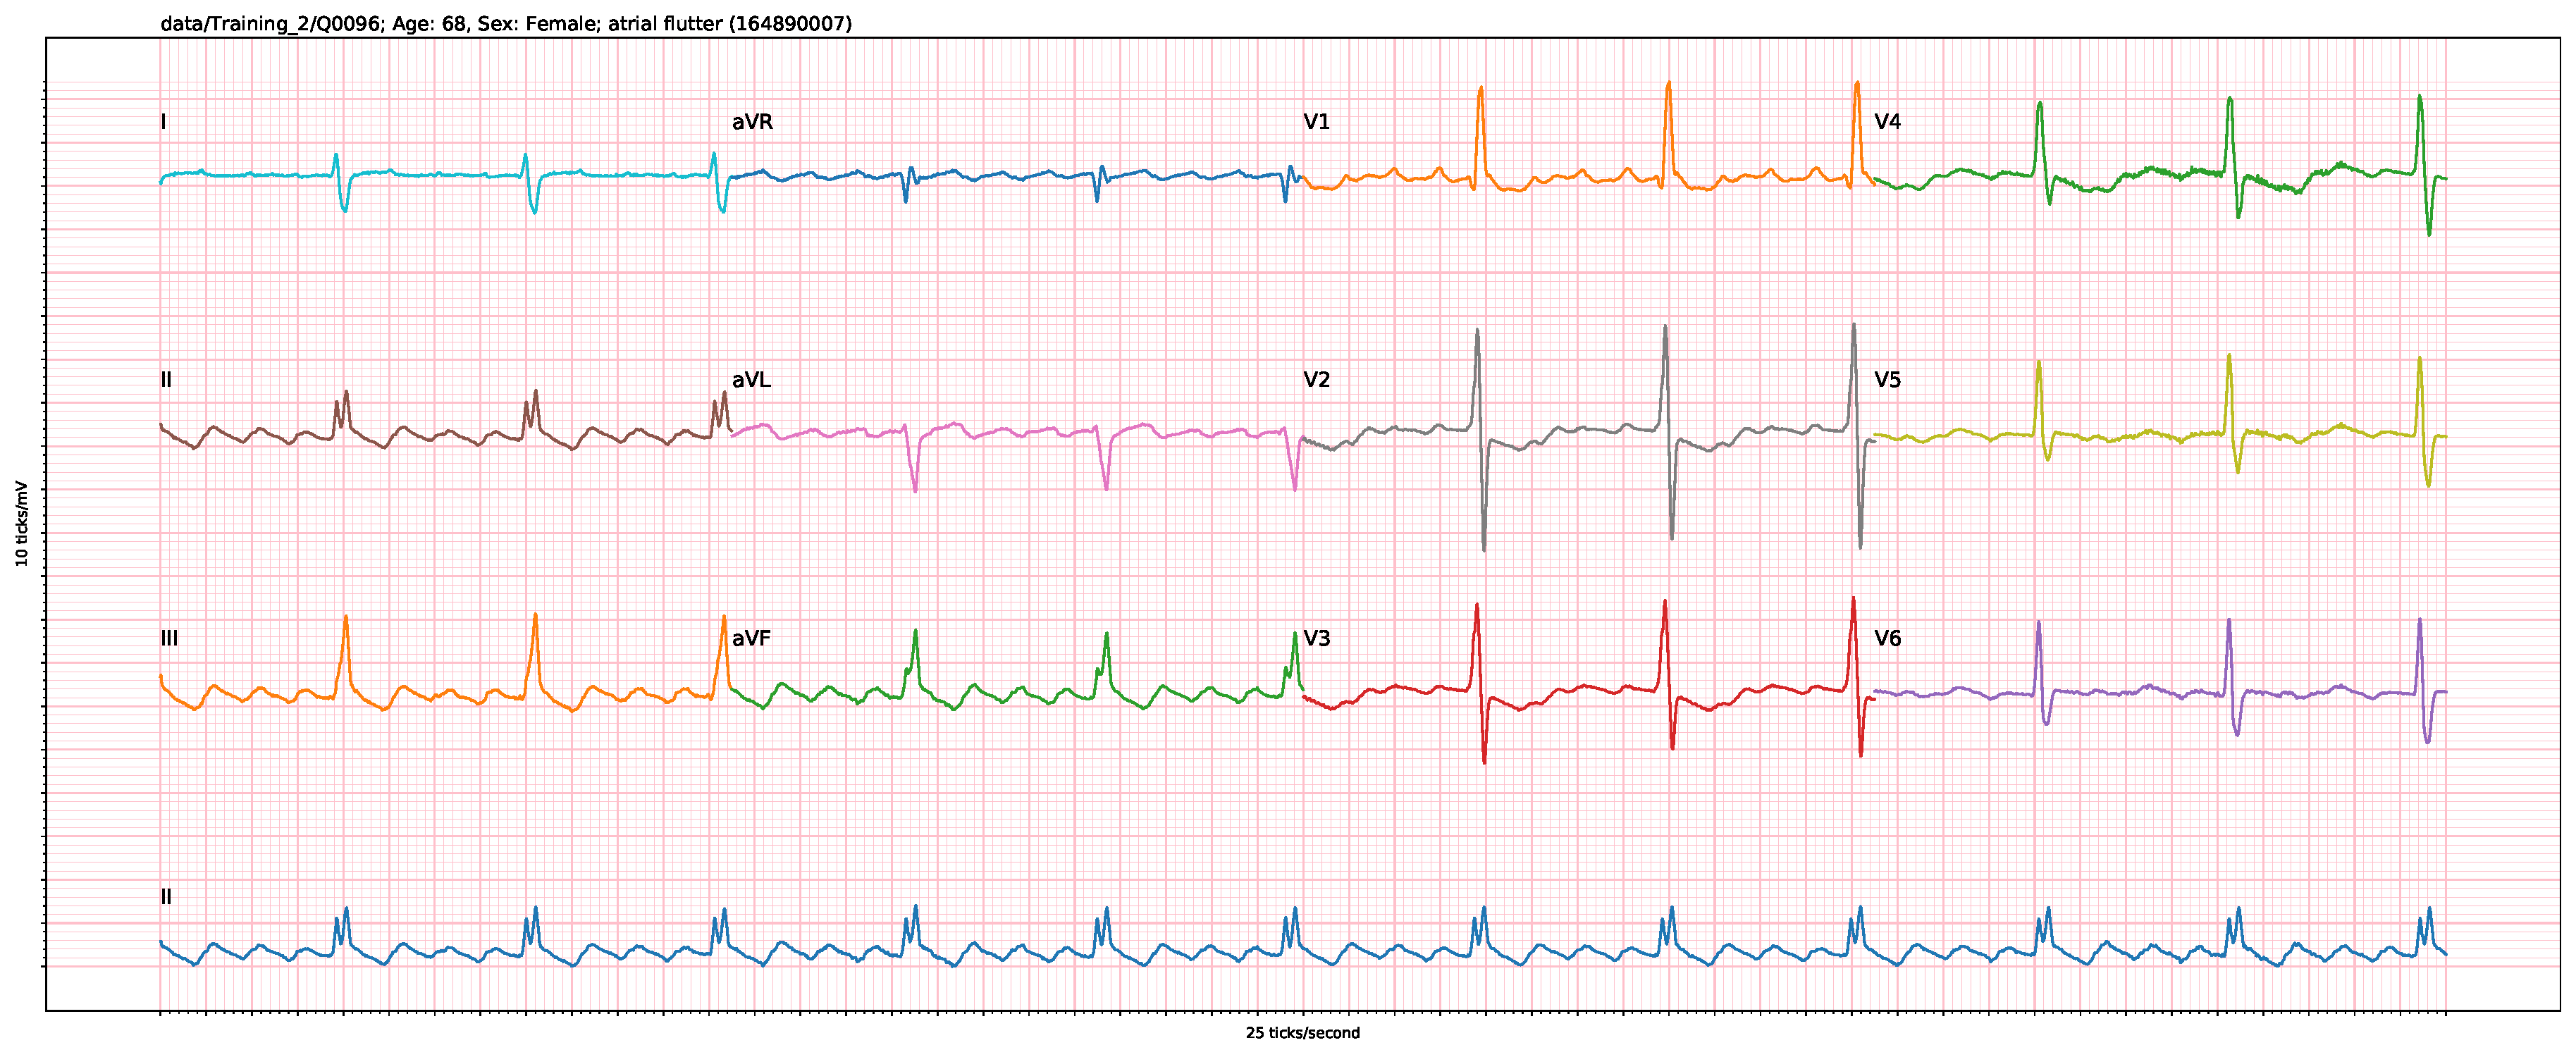
\includegraphics[width=1.2\textwidth]{figure/AFL/full_0_93.pdf}}
        \caption{Instance of 12-lead \gls{ecg} with atrial flutter. Rapid P waves exist.}
        \label{fig:full_AFL}
    \end{figure}
    \item[\gls{afl}] This disorder is indicated by the presence of atrial rhythms at a constant rate $\geq 100$ beats per minute~\cite{saoudi_classification_2001}. Figure~\ref{fig:full_AFL} shows an \gls{ecg} instance with rapid and well-formed P waves.

    \begin{figure}[H]
        \centering
        \makebox[\textwidth][c]{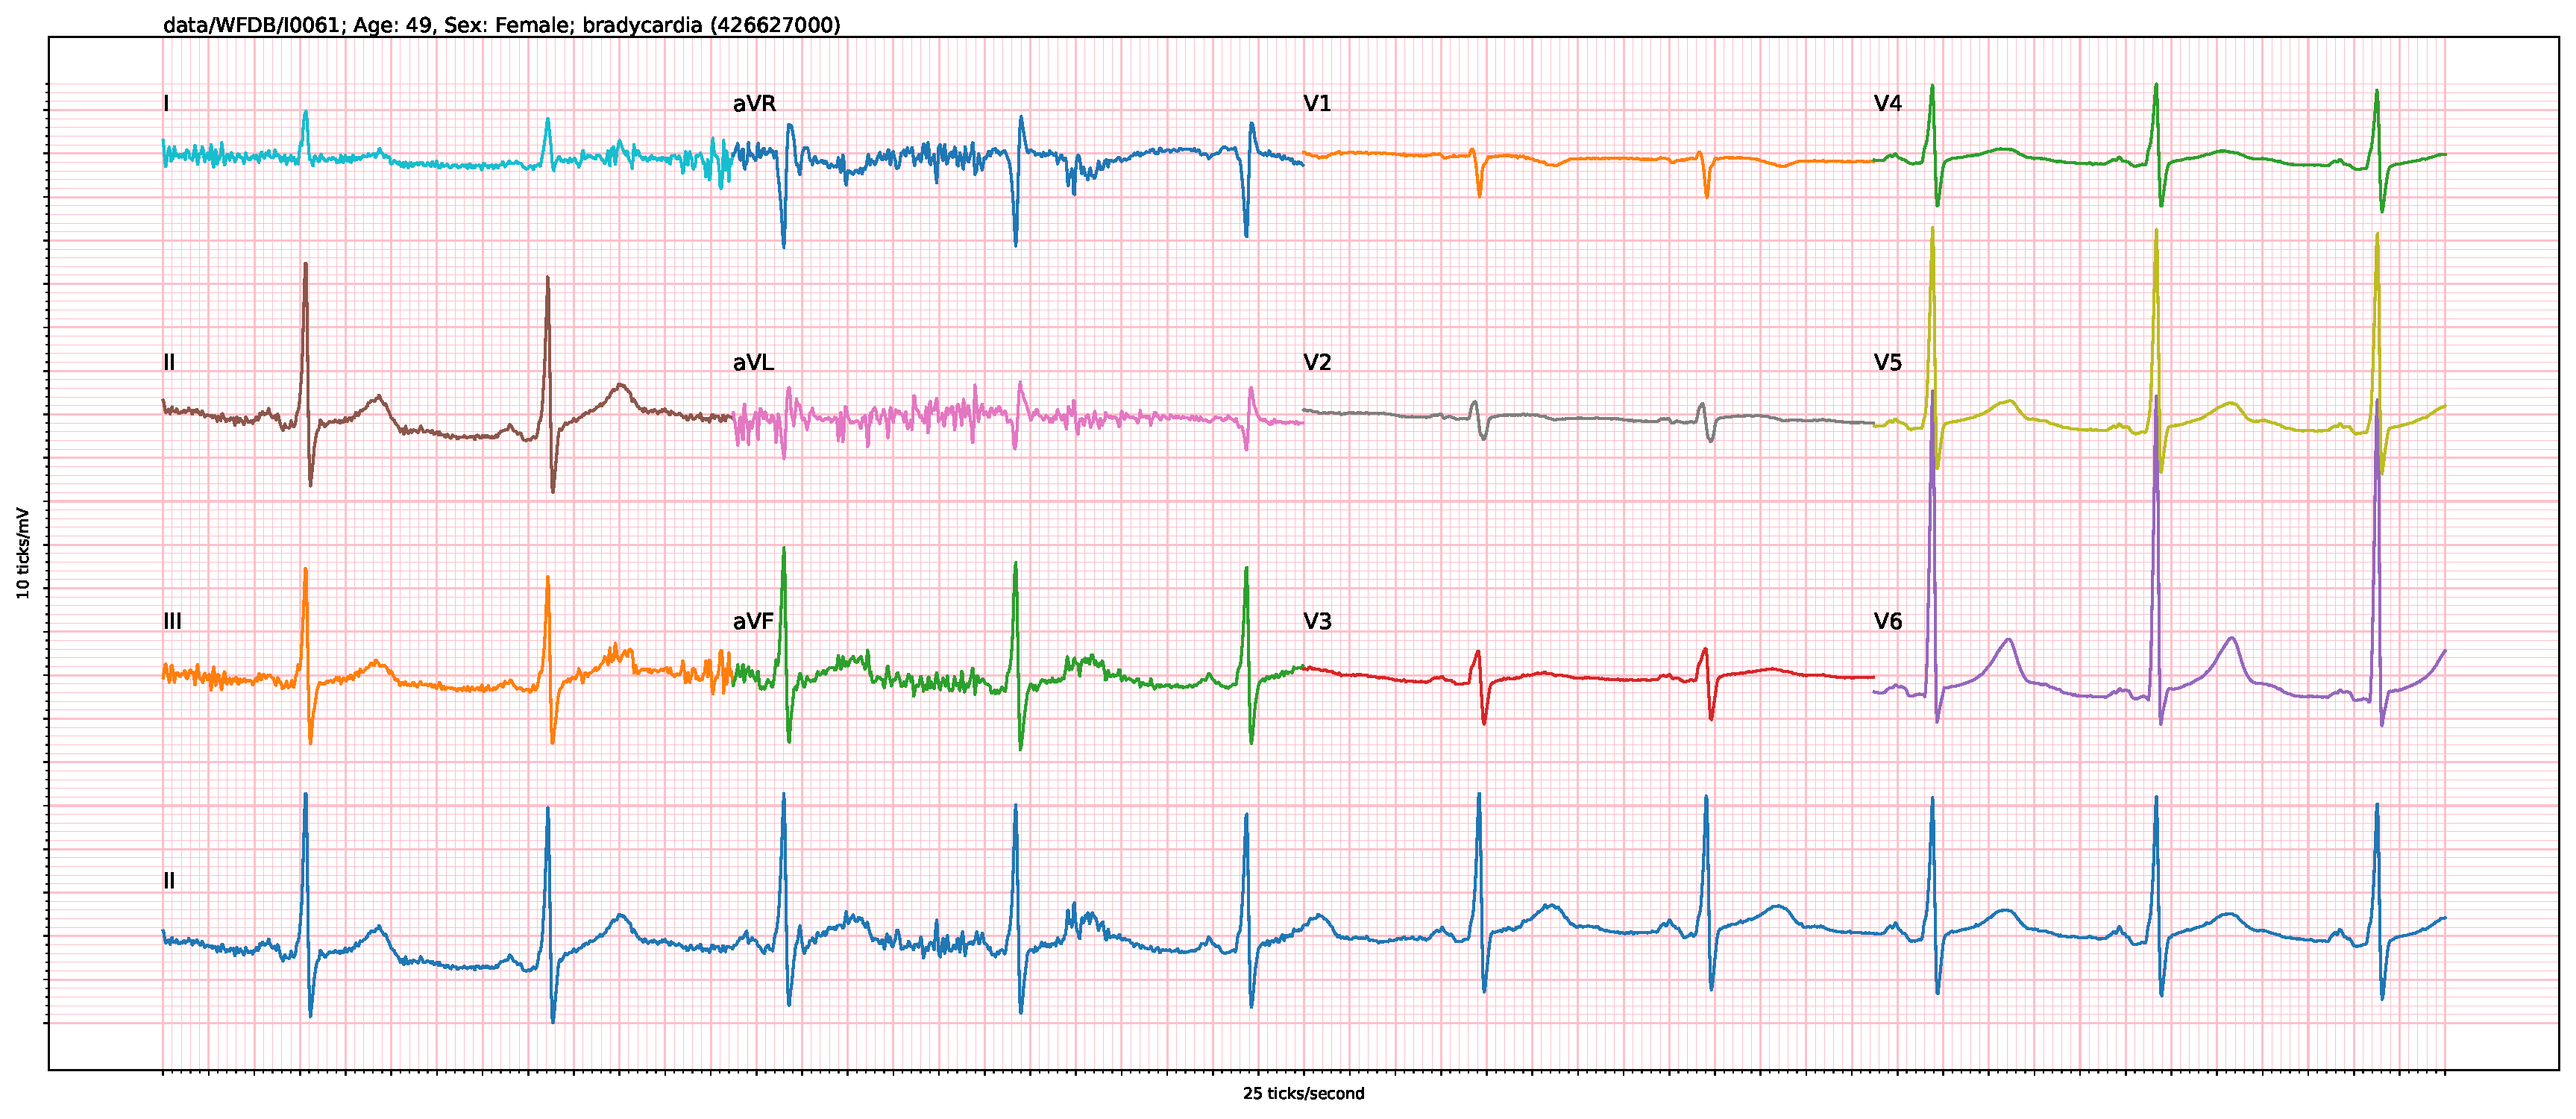
\includegraphics[width=1.2\textwidth]{figure/Brady/full_0_42568.pdf}}
        \caption{Instance of 12-lead \gls{ecg} with bradycardia. Patient has a mean resting heart rate of 57 beats per minute.}
        \label{fig:full_Brady}
    \end{figure} 
    \item[\gls{brady}] A patient has bradycardia if their sinus rhythm is below the normal range of for the age of the patient. For adults, this is a resting heart rate below 60 beats per minute. An example of a patient with bradycardia is shown in Figure~\ref{fig:full_Brady}.

    \begin{figure}[H]
        \centering
        \makebox[\textwidth][c]{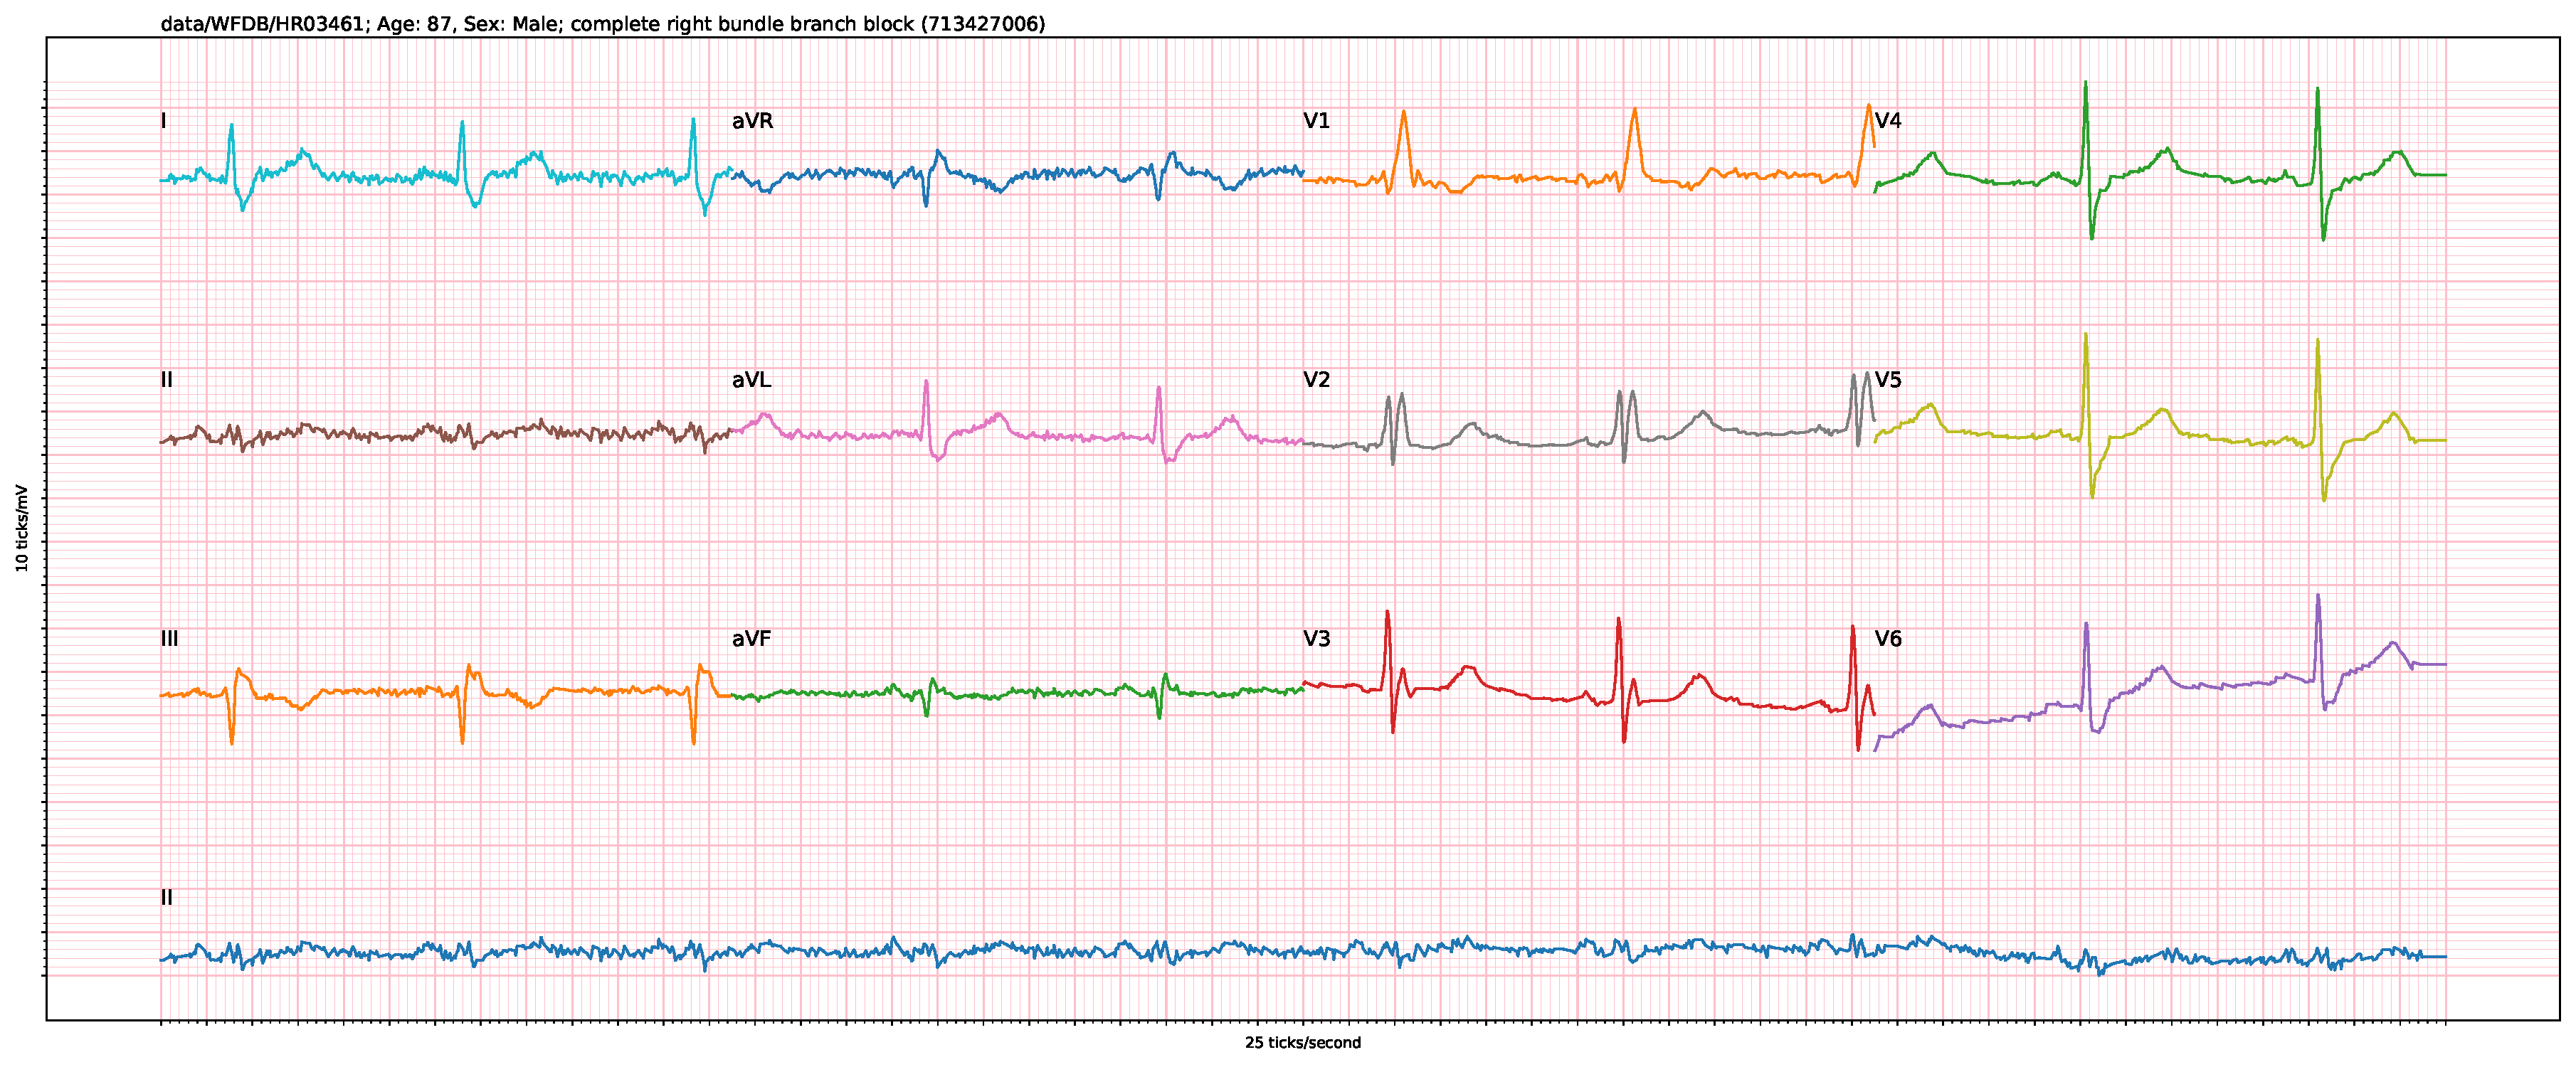
\includegraphics[width=1.2\textwidth]{figure/CRBBB/full_2_24132.pdf}}
        \caption{Instance of 12-lead \gls{ecg} with complete right bundle branch block. QRS complex exceeds 120 ms (4 boxes) and contains an anterior skew on the right end of the QRS complex.}
        \label{fig:full_CRBBB}
    \end{figure} 
    \item[\gls{crbbb}] A complete right bundle branch block is when the QRS duration exceeds 120 ms and the terminal halves of the QRS are skewed rightward and anteriorly, indicating that the right ventricle is being depolarized after the left ventricle~\cite{ecg-utah-lesson}. An example \gls{ecg} record is shown in Figure~\ref{fig:full_CRBBB}.

    \begin{figure}[H]
        \centering
        \makebox[\textwidth][c]{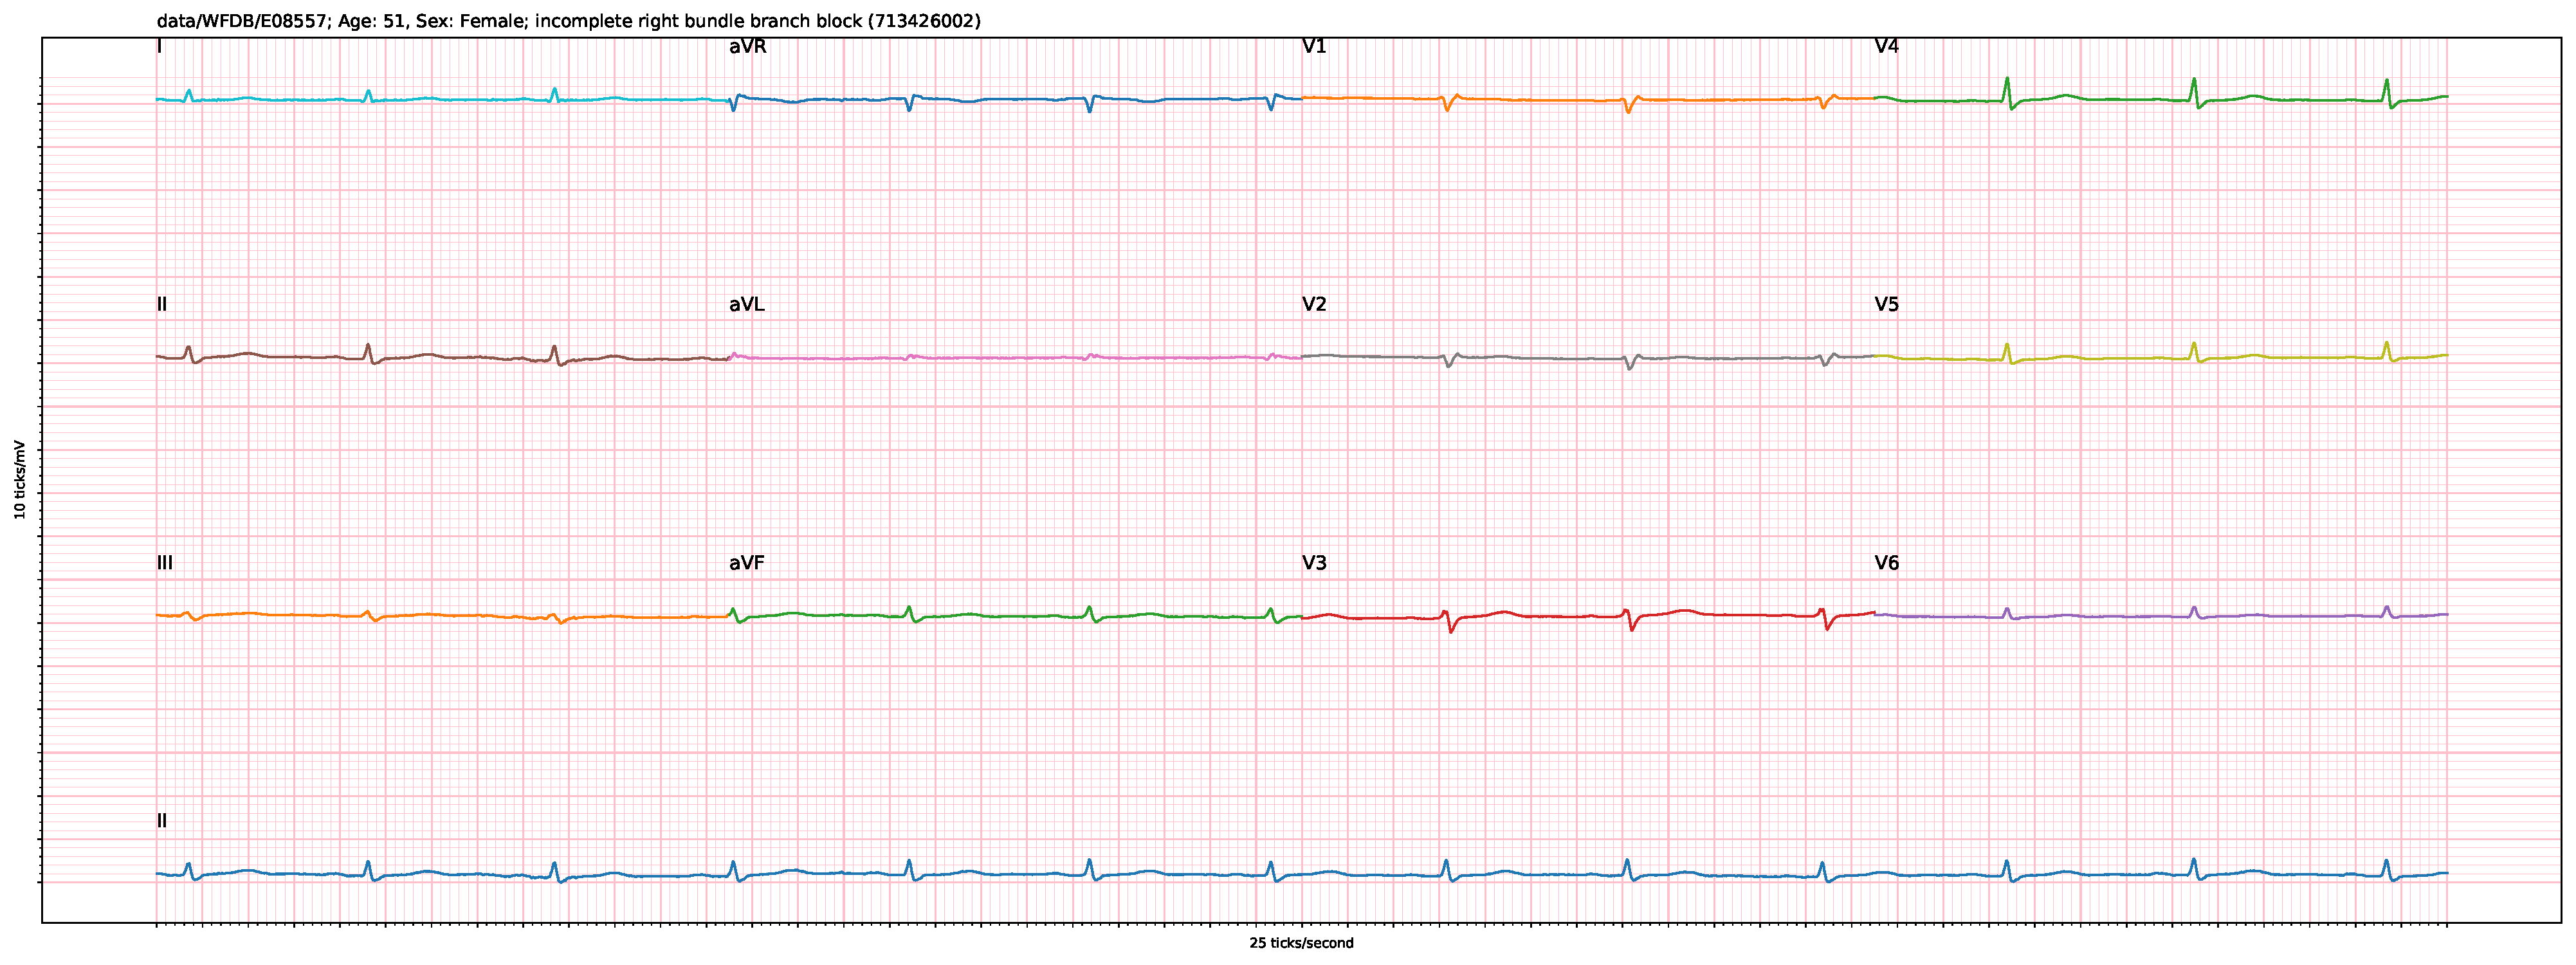
\includegraphics[width=1.2\textwidth]{figure/IRBBB/full_28_18884.pdf}}
        \caption{Instance of 12-lead \gls{ecg} with incomplete right bundle branch block. The QRS complex is within 100 to 120 ms (2.5-3 boxes) and contains an anterior skew on the right end of the QRS complex.}
        \label{fig:full_IRBBB}
    \end{figure} 
    \item[\gls{irbbb}] An incomplete right bundle branch block has the same terminal QRS features as \gls{crbbb} but has a QRS duration of 100 to 120 ms~\cite{ecg-utah-lesson}, as shown in the example record at Figure~\ref{fig:full_IRBBB}.

    \begin{figure}[H]
        \centering
        \makebox[\textwidth][c]{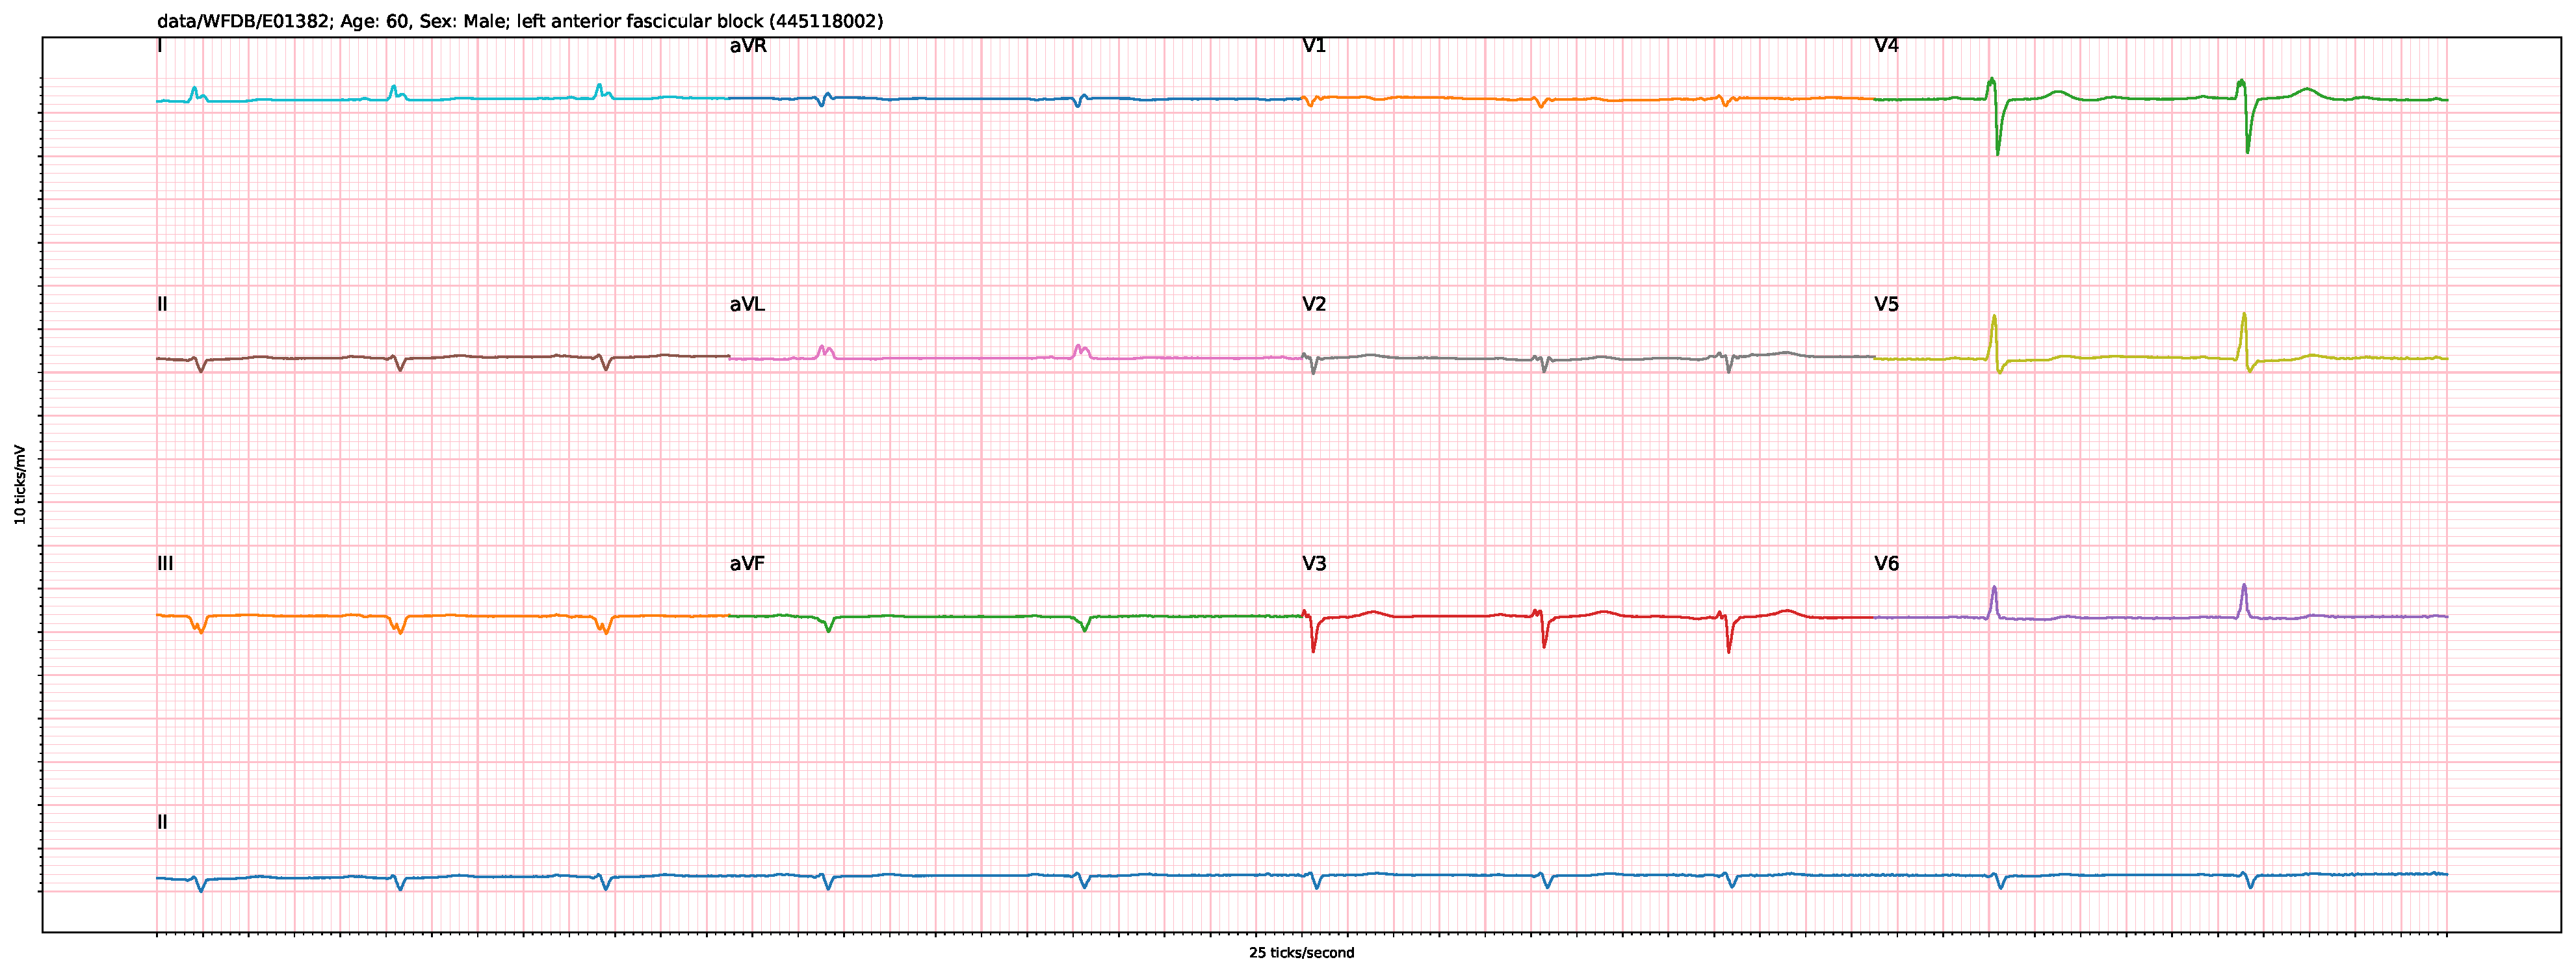
\includegraphics[width=1.2\textwidth]{figure/LAnFB/full_3_11709.pdf}}
        \caption{Instance of 12-lead \gls{ecg} with left anterior fascicular block. Lead I is positive while leads II and III are negative, indicating left axis deviation. Leads I and aVL show qR complexes, with rS complexes appearing in leads II, III, an aVF.}
        \label{fig:full_LAnFB}
    \end{figure} 
    \item[\gls{lanfb}] This common intraventricular defect occurs when the anterior fascicle within the left bundle branch is blocked or otherwise unable to respond to action potential stimuli~\cite{ecg-utah-lesson}. The criteria includes: left axis deviation (within $-45\degree$ to $-90\degree$); small Q waves with large R waves (`qR complexes') in leads I and/or aVL; small R waves with deep S waves (`rS complexes') in leads II, III, and aVF; slightly prolonged QRS duration (80-110ms), usually a poor R progression in leads V1, V2, and V3 with deeper S waves in leads V5 and V6. See Figure~\ref{fig:full_LAnFB} for an example.

    \begin{figure}[H]
        \centering
        \makebox[\textwidth][c]{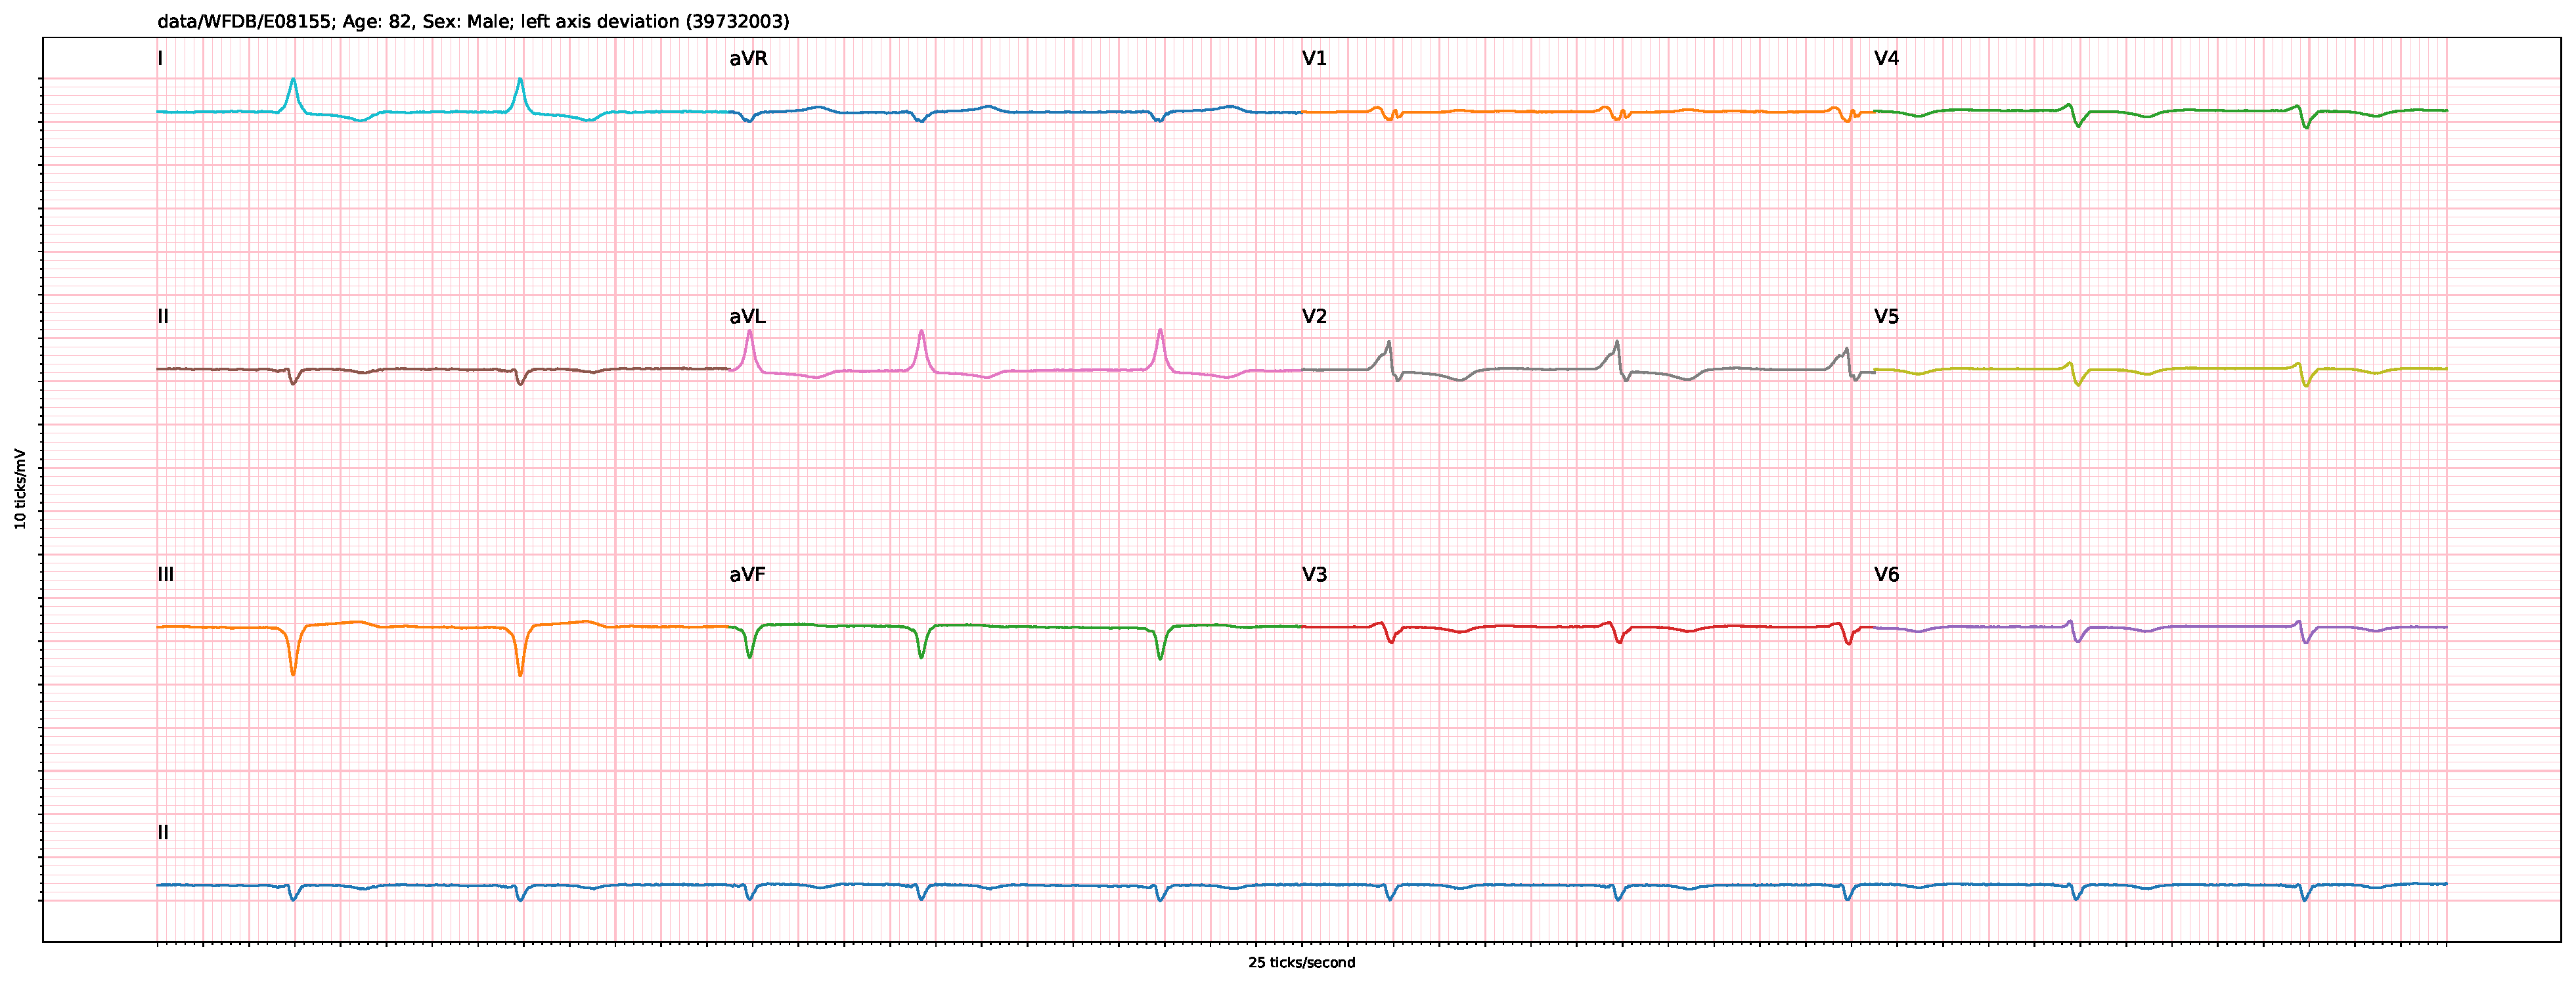
\includegraphics[width=1.2\textwidth]{figure/LAD/full_69_18482.pdf}}
        \caption{Instance of 12-lead \gls{ecg} with left axis deviation. Lead I is positive while leads II and III are negative, indicating left axis deviation using the simple leads I, II, III method. Using the hexaxial axis estimation approach, we see that leads aVL and III have the greatest QRS complex magnitude with aVL being positive and III being negative, giving an electrical axis between $-30\degree$ and $-60\degree$, confirming left axis deviation.}
        \label{fig:full_LAD}
    \end{figure}
    \item[\gls{lad}] Diagnosed when the cardiac axis exists between $-30\degree$ and $-90\degree$. See Figure~\ref{fig:full_LAD} for an example \gls{ecg} record, interpreted using the lead I, II, III approach as well as the hexaxial reference system.

    \begin{figure}[H]
        \centering
        \makebox[\textwidth][c]{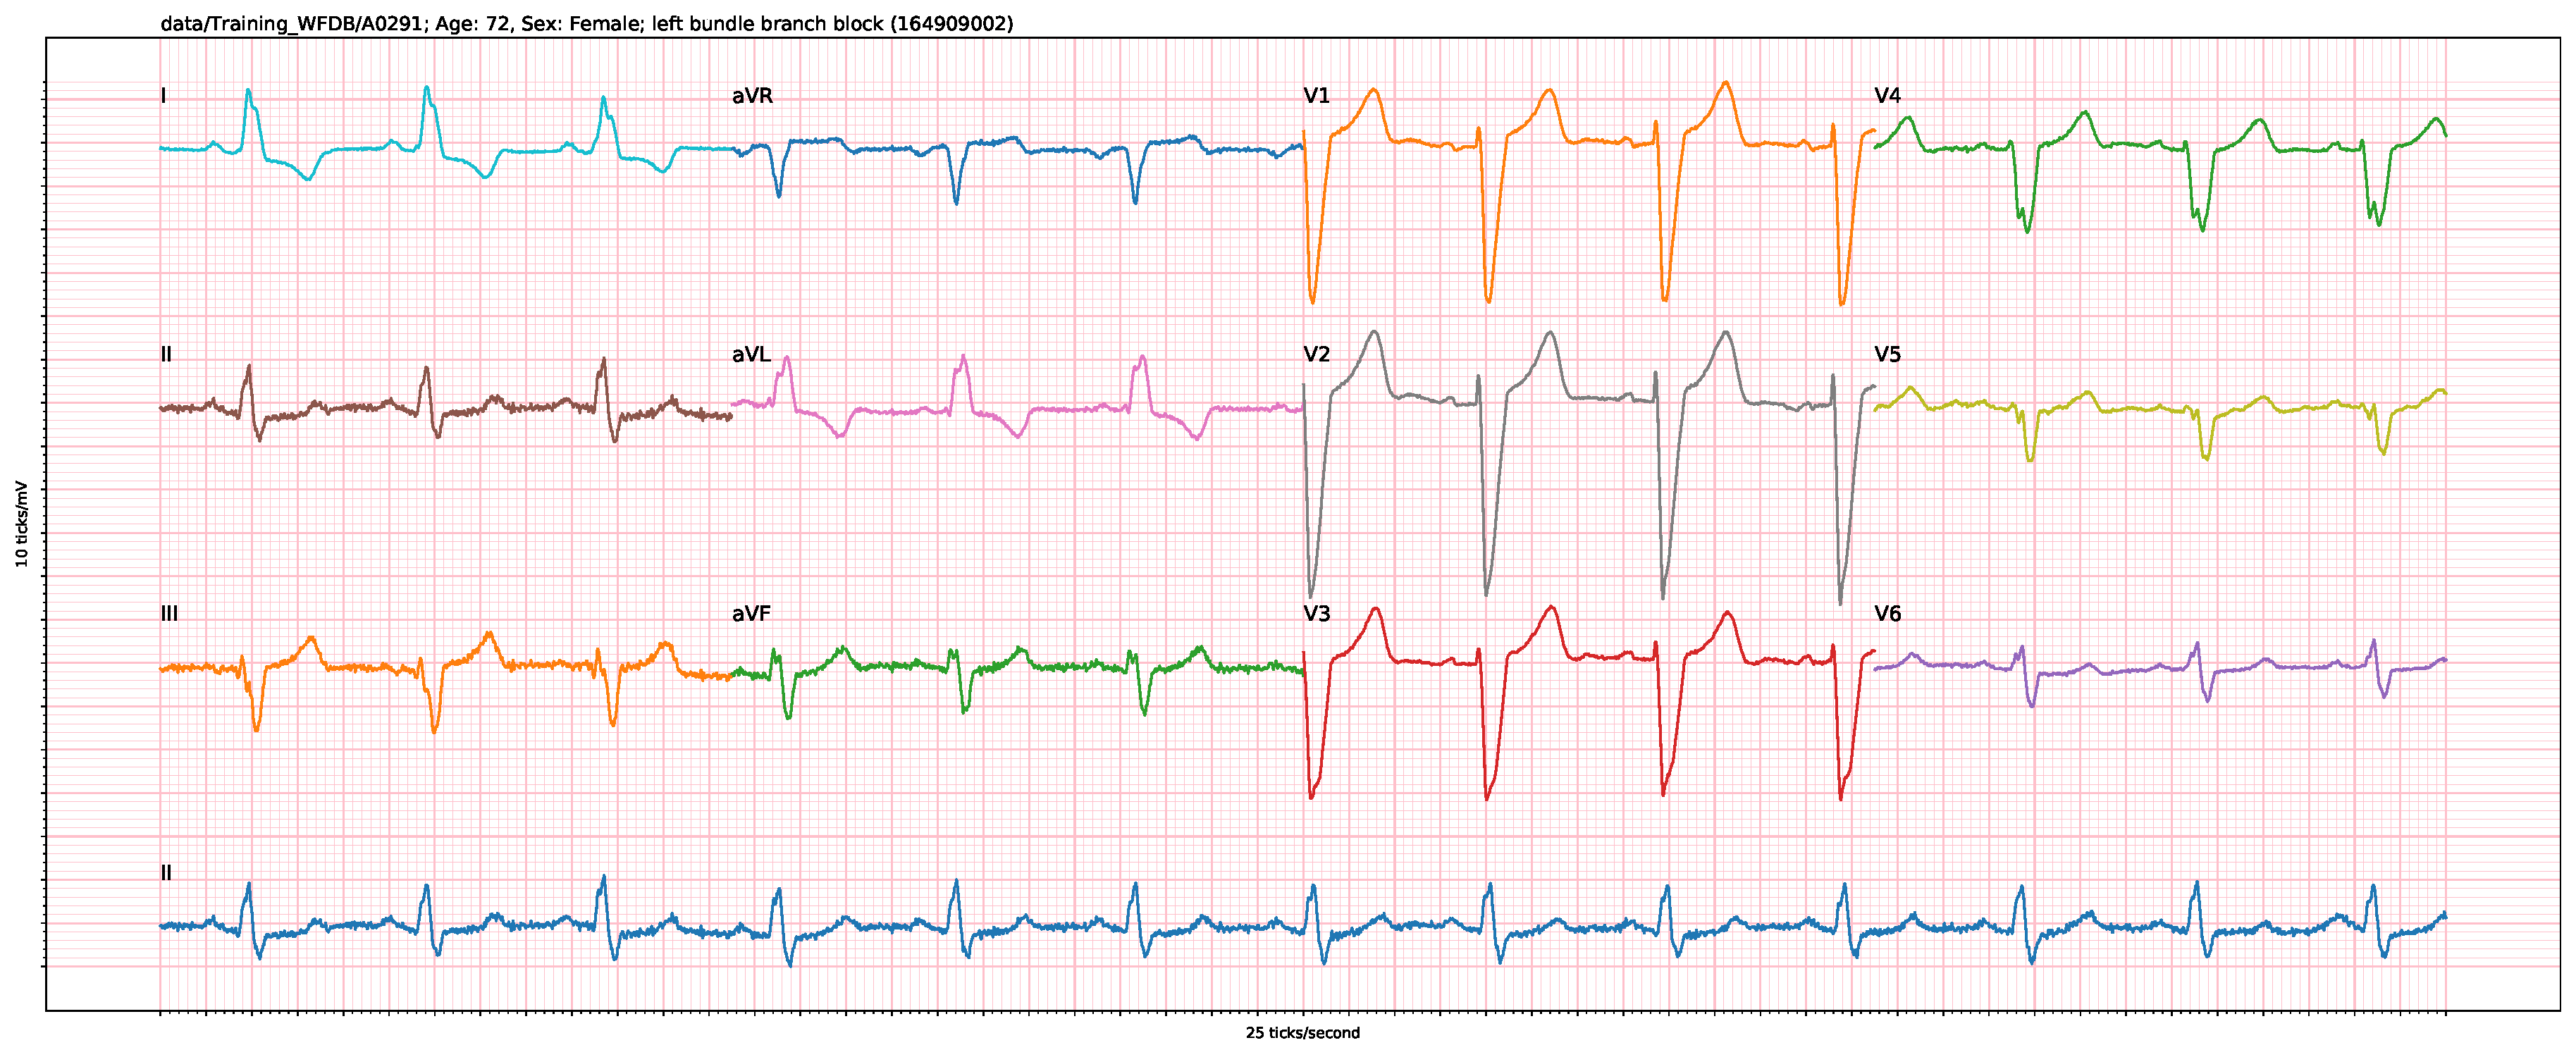
\includegraphics[width=1.2\textwidth]{figure/LBBB/full_10_3741.pdf}}
        \caption{Instance of 12-lead \gls{ecg} with left bundle branch block. The QRS complexes exceed 100ms (2.5 boxes) and contain a posterior or leftward skew on the tail halves of the QRS complexes.}
        \label{fig:full_LBBB}
    \end{figure}
    \item[\gls{lbbb}] A left bundle branch block is defined by a QRS complex exceeding 100ms with a posterior/leftward skew in the second half of the QRS complex~\cite{ecg-utah-lesson}. An example record is shown in Figure~\ref{fig:full_LBBB}. For the purposes of this challenge, no distinction is made between complete left bundle branch block ($> 120$ms) and incomplete left bundle branch block (between 100ms and 120ms).

    \begin{figure}[H]
        \centering
        \makebox[\textwidth][c]{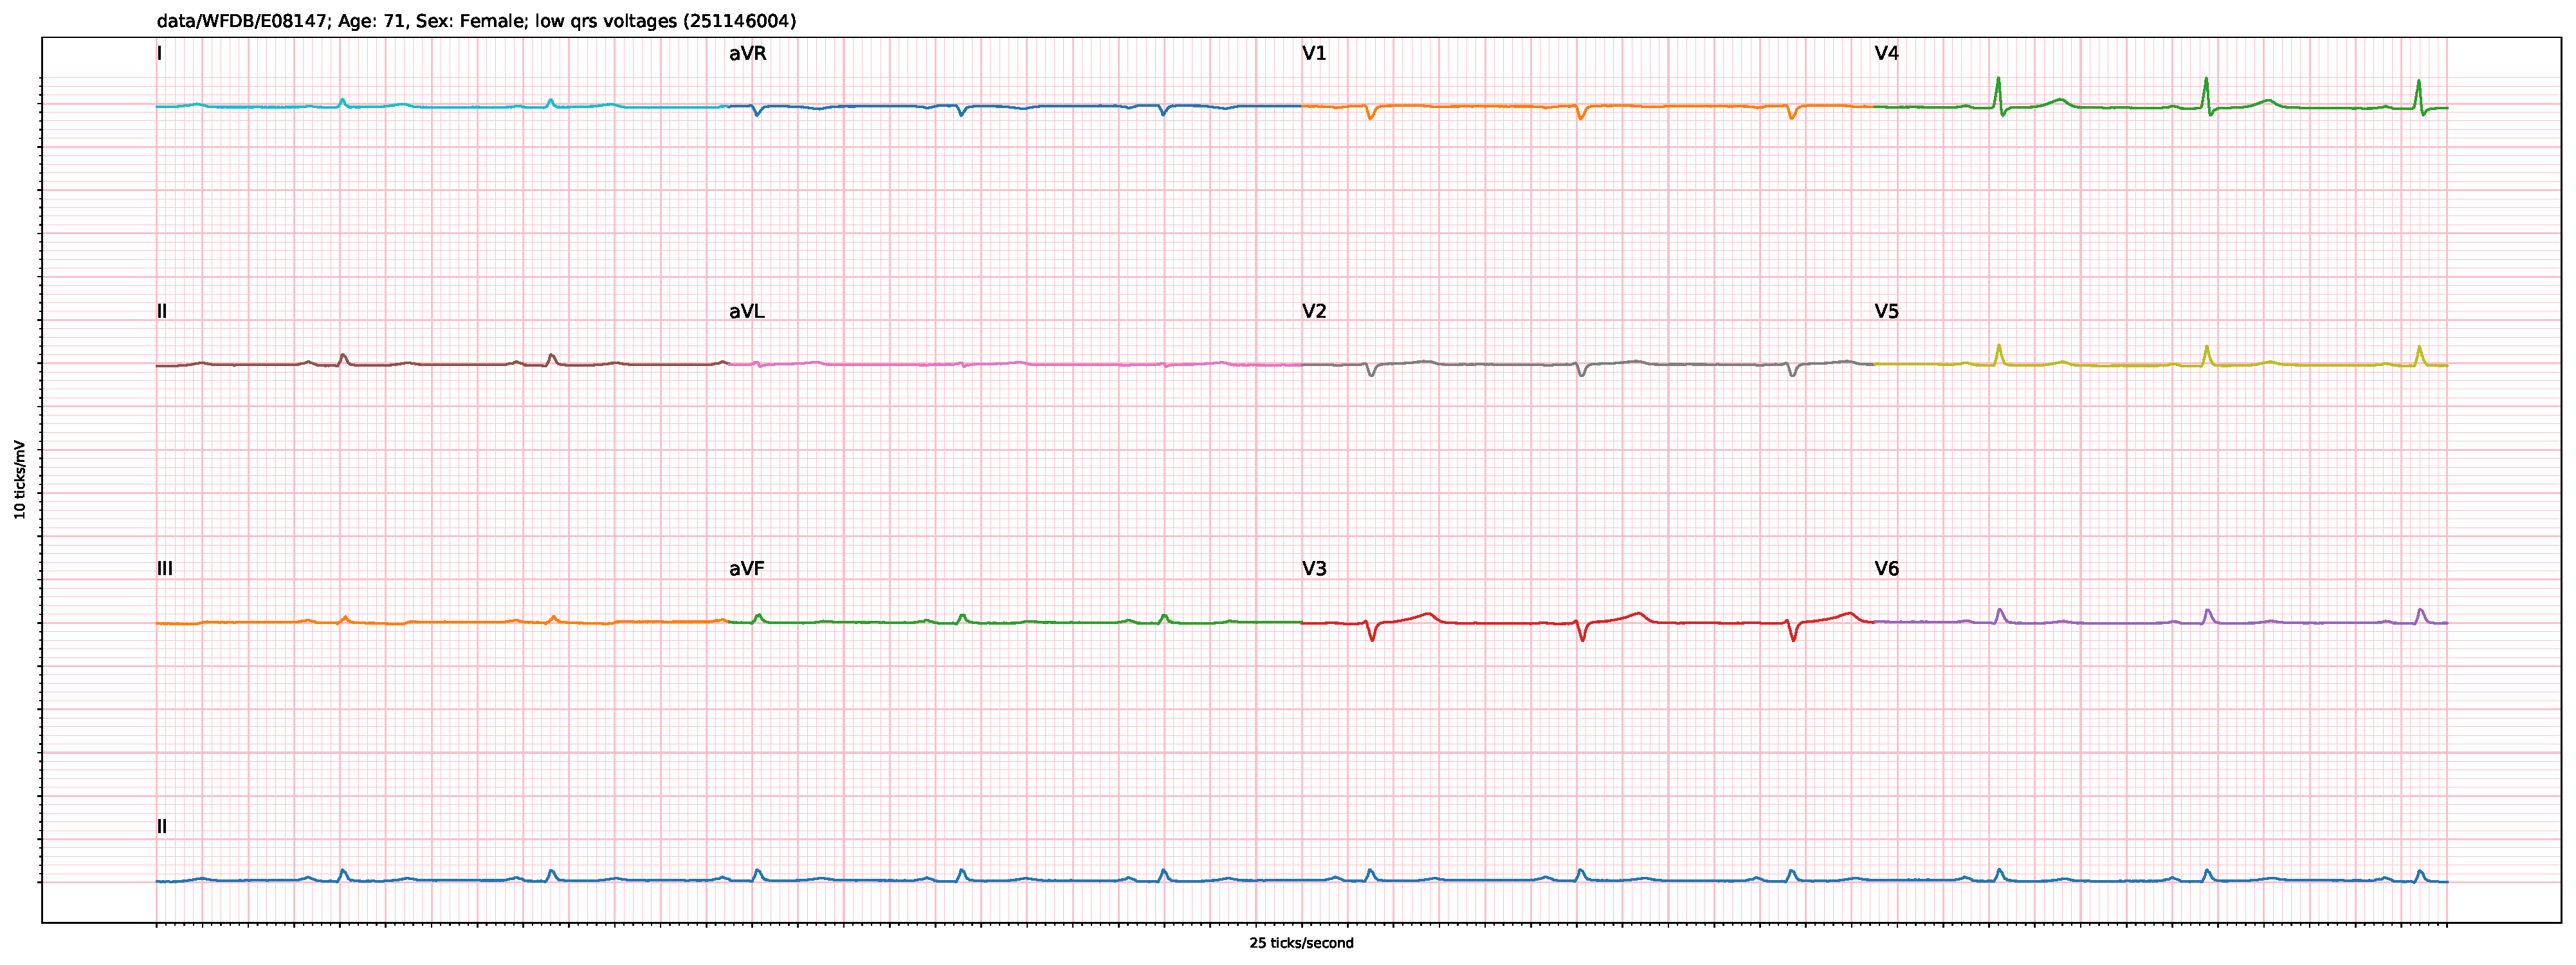
\includegraphics[width=1.2\textwidth]{figure/LQRSV/full_53_18474.pdf}}
        \caption{Instance of 12-lead \gls{ecg} with low QRS voltages. All limb leads have QRS complex amplitudes of less than 0.5mV and all precordial leads have QRS complex amplitudes of less than 1.0mV.}
        \label{fig:full_LQRSV}
    \end{figure}
    \item[\gls{lqrsv}] An \gls{ecg} record with low QRS voltages contains QRS complex amplitudes of $<$ 0.5mV in all limb derived leads (I, II, III, aVR, aVL, aVF) or contains QRS complex amplitudes of $<$ 1mV in all precordial leads (V1, V2, V3, V4, V5, V6)~\cite{madias_low_2008}. See Figure~\ref{fig:full_LQRSV} for an example.

    \begin{figure}[H]
        \centering
        \makebox[\textwidth][c]{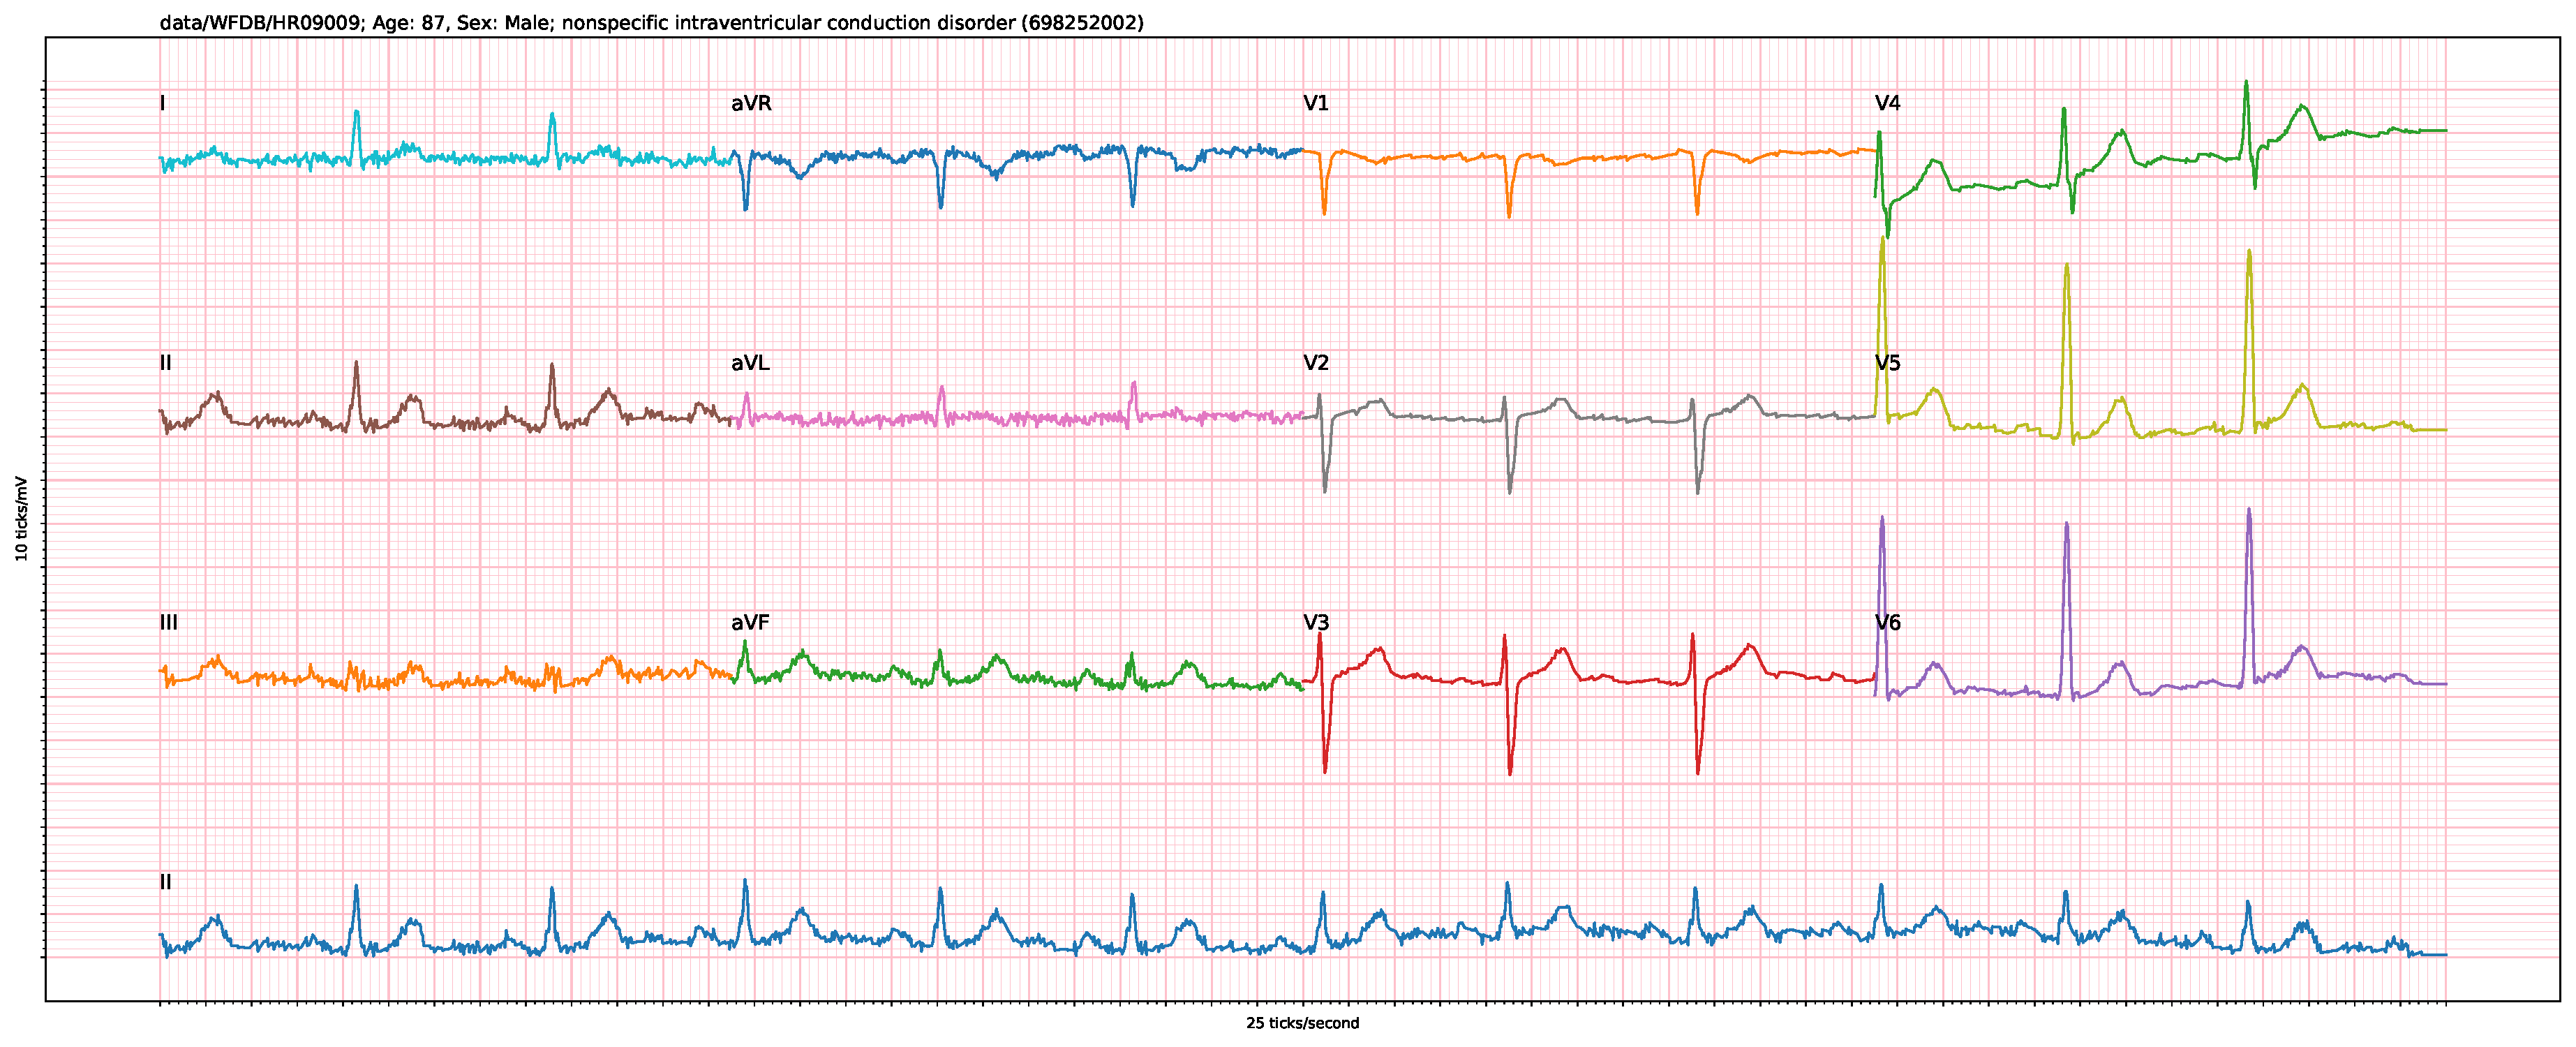
\includegraphics[width=1.2\textwidth]{figure/NSIVCB/full_12_29680.pdf}}
        \caption{Instance of 12-lead \gls{ecg} with nonspecific intraventricular conduction disorder. QRS complexes exceed 100ms (2.5 squares) but do not exhibit a posterior/anterior skew characteristic on the tail half of the QRS complexes.}
        \label{fig:full_NSIVCB}
    \end{figure}
    \item[\gls{nsivcb}] An \gls{ecg} record with nonspecific intraventricular conduction blocks exhibits QRS durations over 100ms but do not contain a posterior/anterior skew characteristic on the second half of the QRS complex~\cite{ecg-utah-lesson}.
    An example can be found in Figure~\ref{fig:full_NSIVCB}.

    \begin{figure}[H]
        \centering
        \makebox[\textwidth][c]{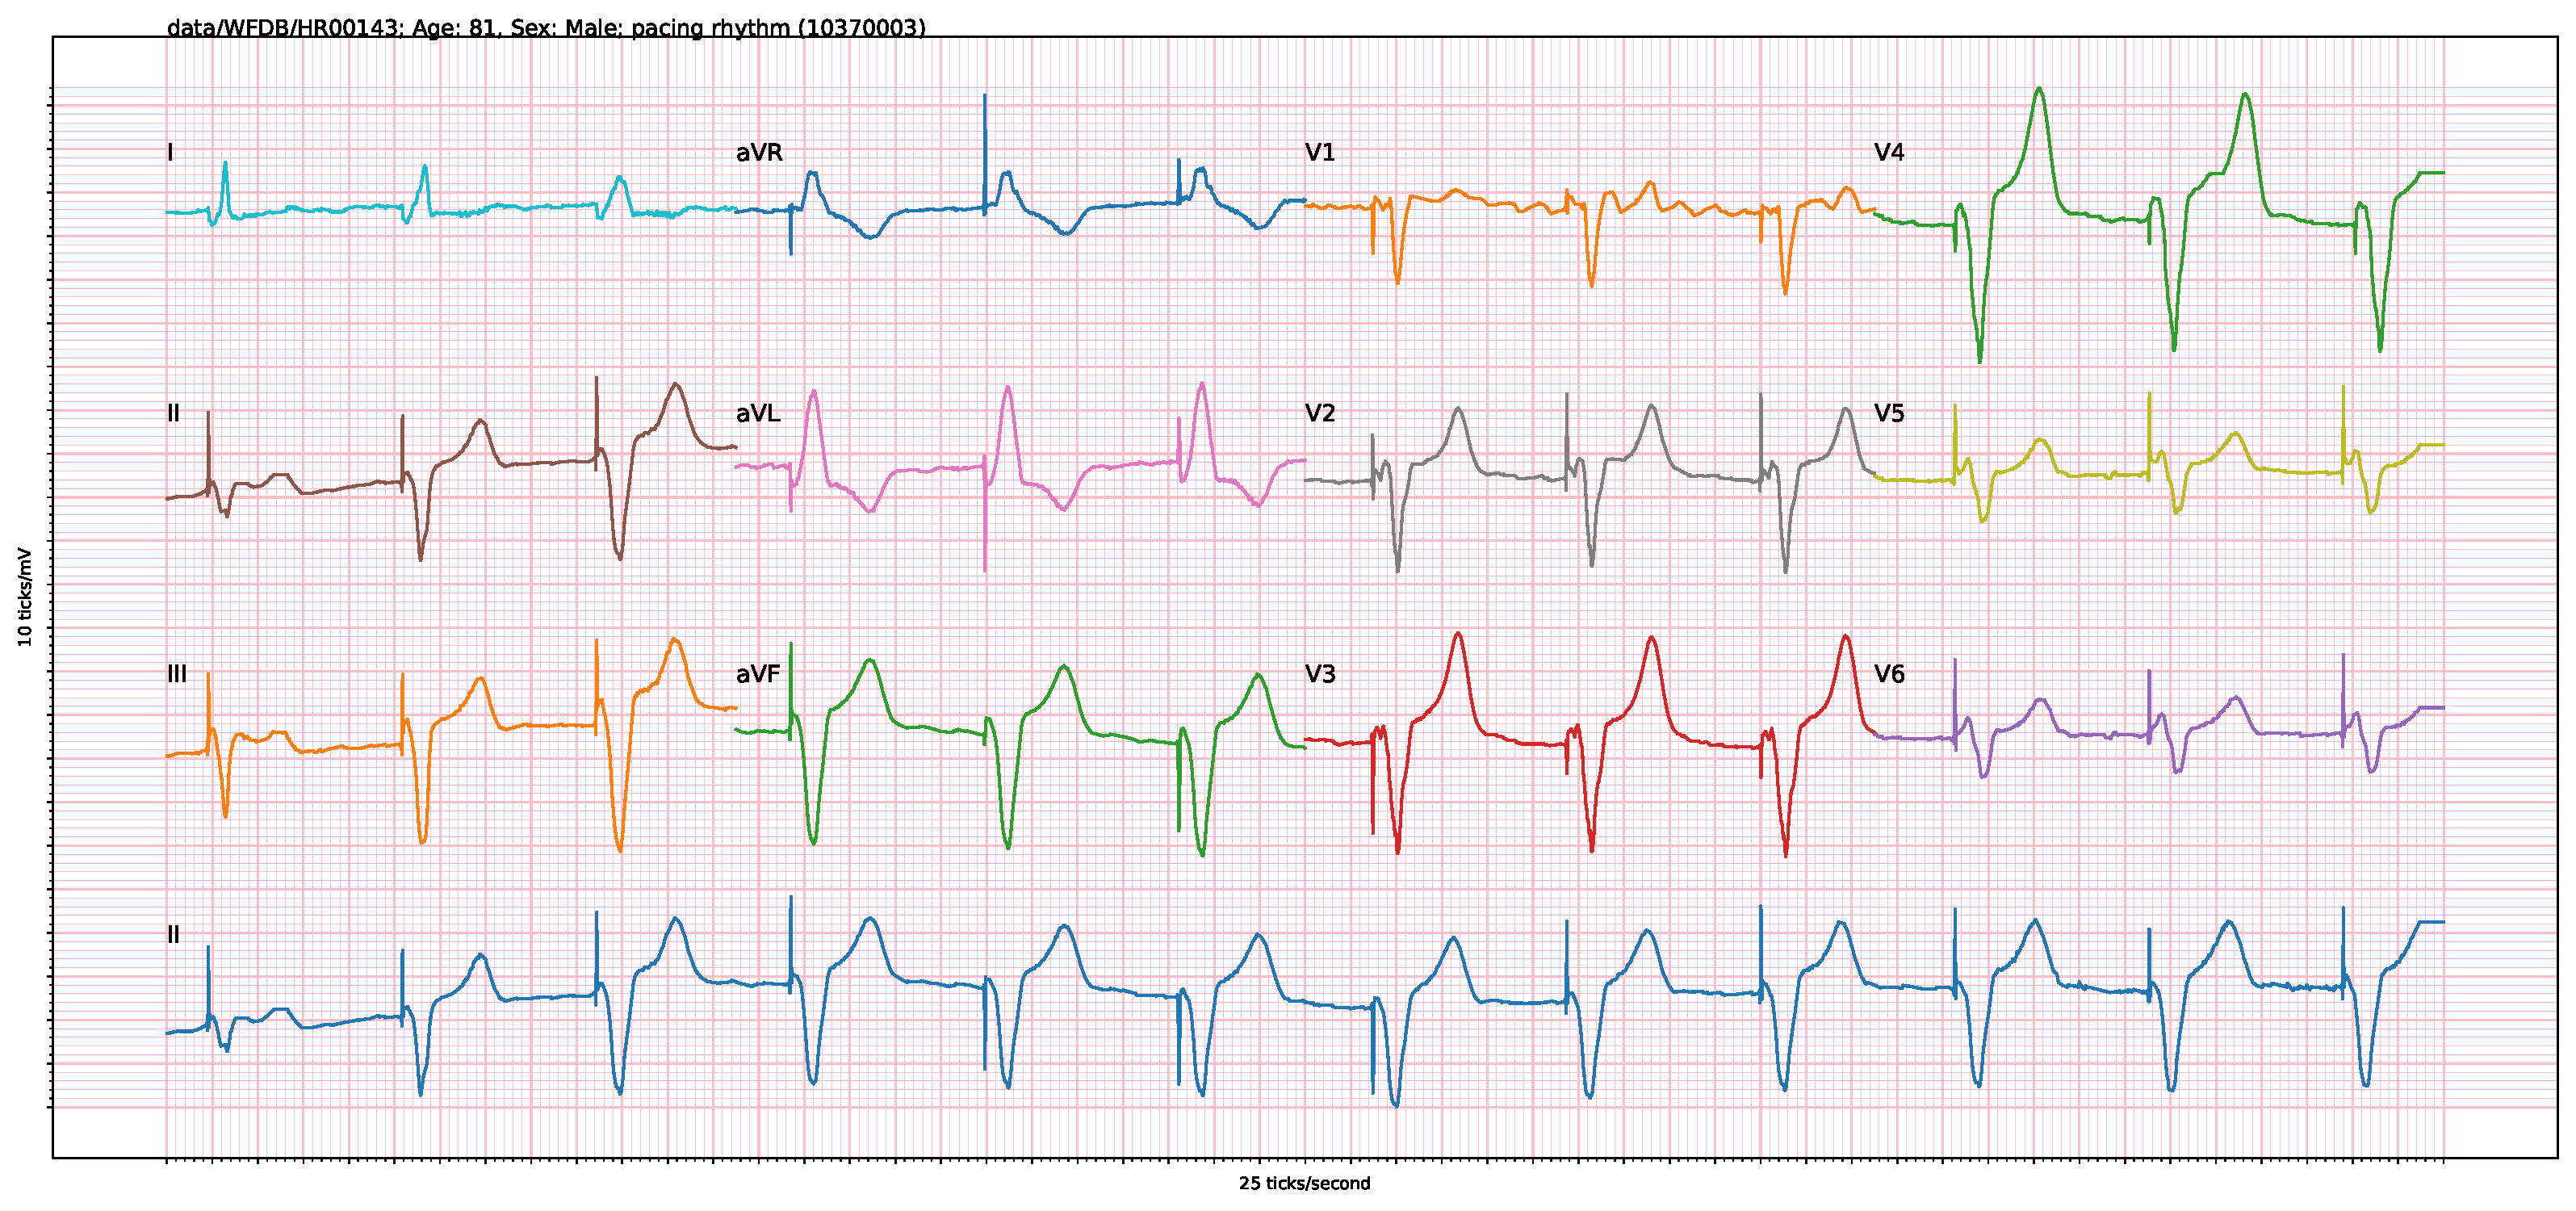
\includegraphics[width=1.2\textwidth]{figure/PR/full_0_20814.pdf}}
        \caption{Instance of 12-lead \gls{ecg} with pacing rhythm. Characteristic vertical lines appearing at the P wave onset suggests atrial pacing with normal conduction to the ventricles.}
        \label{fig:full_PR}
    \end{figure}
    \item[\gls{pr}] This diagnosis indicates the presence of a pacemaker. One common artifact is a vertical line appearing in the \gls{ecg} prior to the QRS complex~\cite{kirk_basic_2007}.
    An example \gls{ecg} record can be found in Figure~\ref{fig:full_PR}.

    \begin{figure}[H]
        \centering
        % \makebox[\textwidth][c]{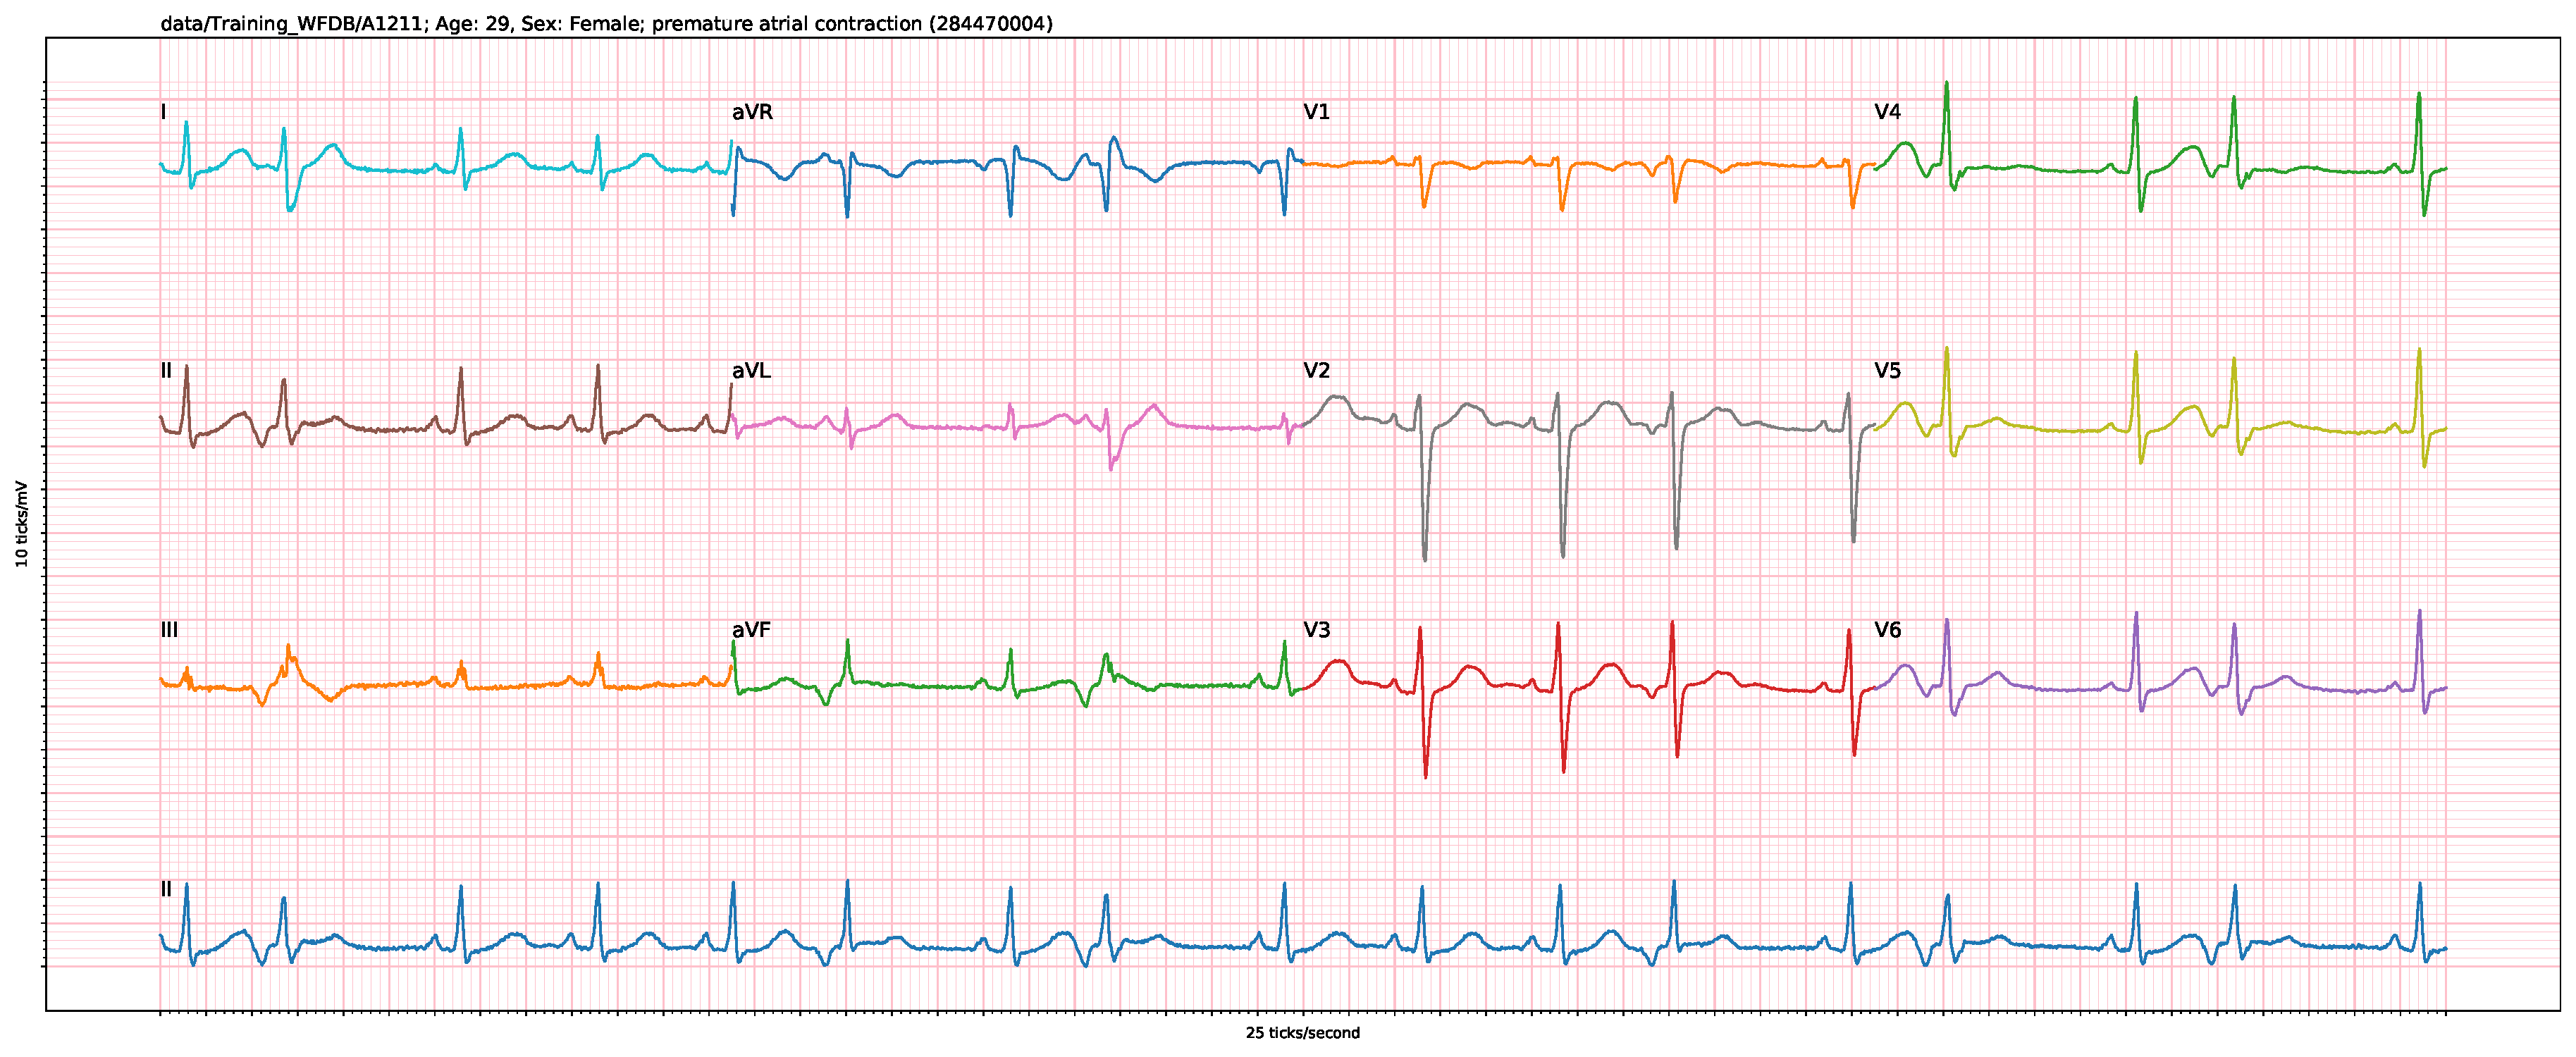
\includegraphics[width=1.2\textwidth]{figure/PAC/full_95_4661.pdf}}
        \makebox[\textwidth][c]{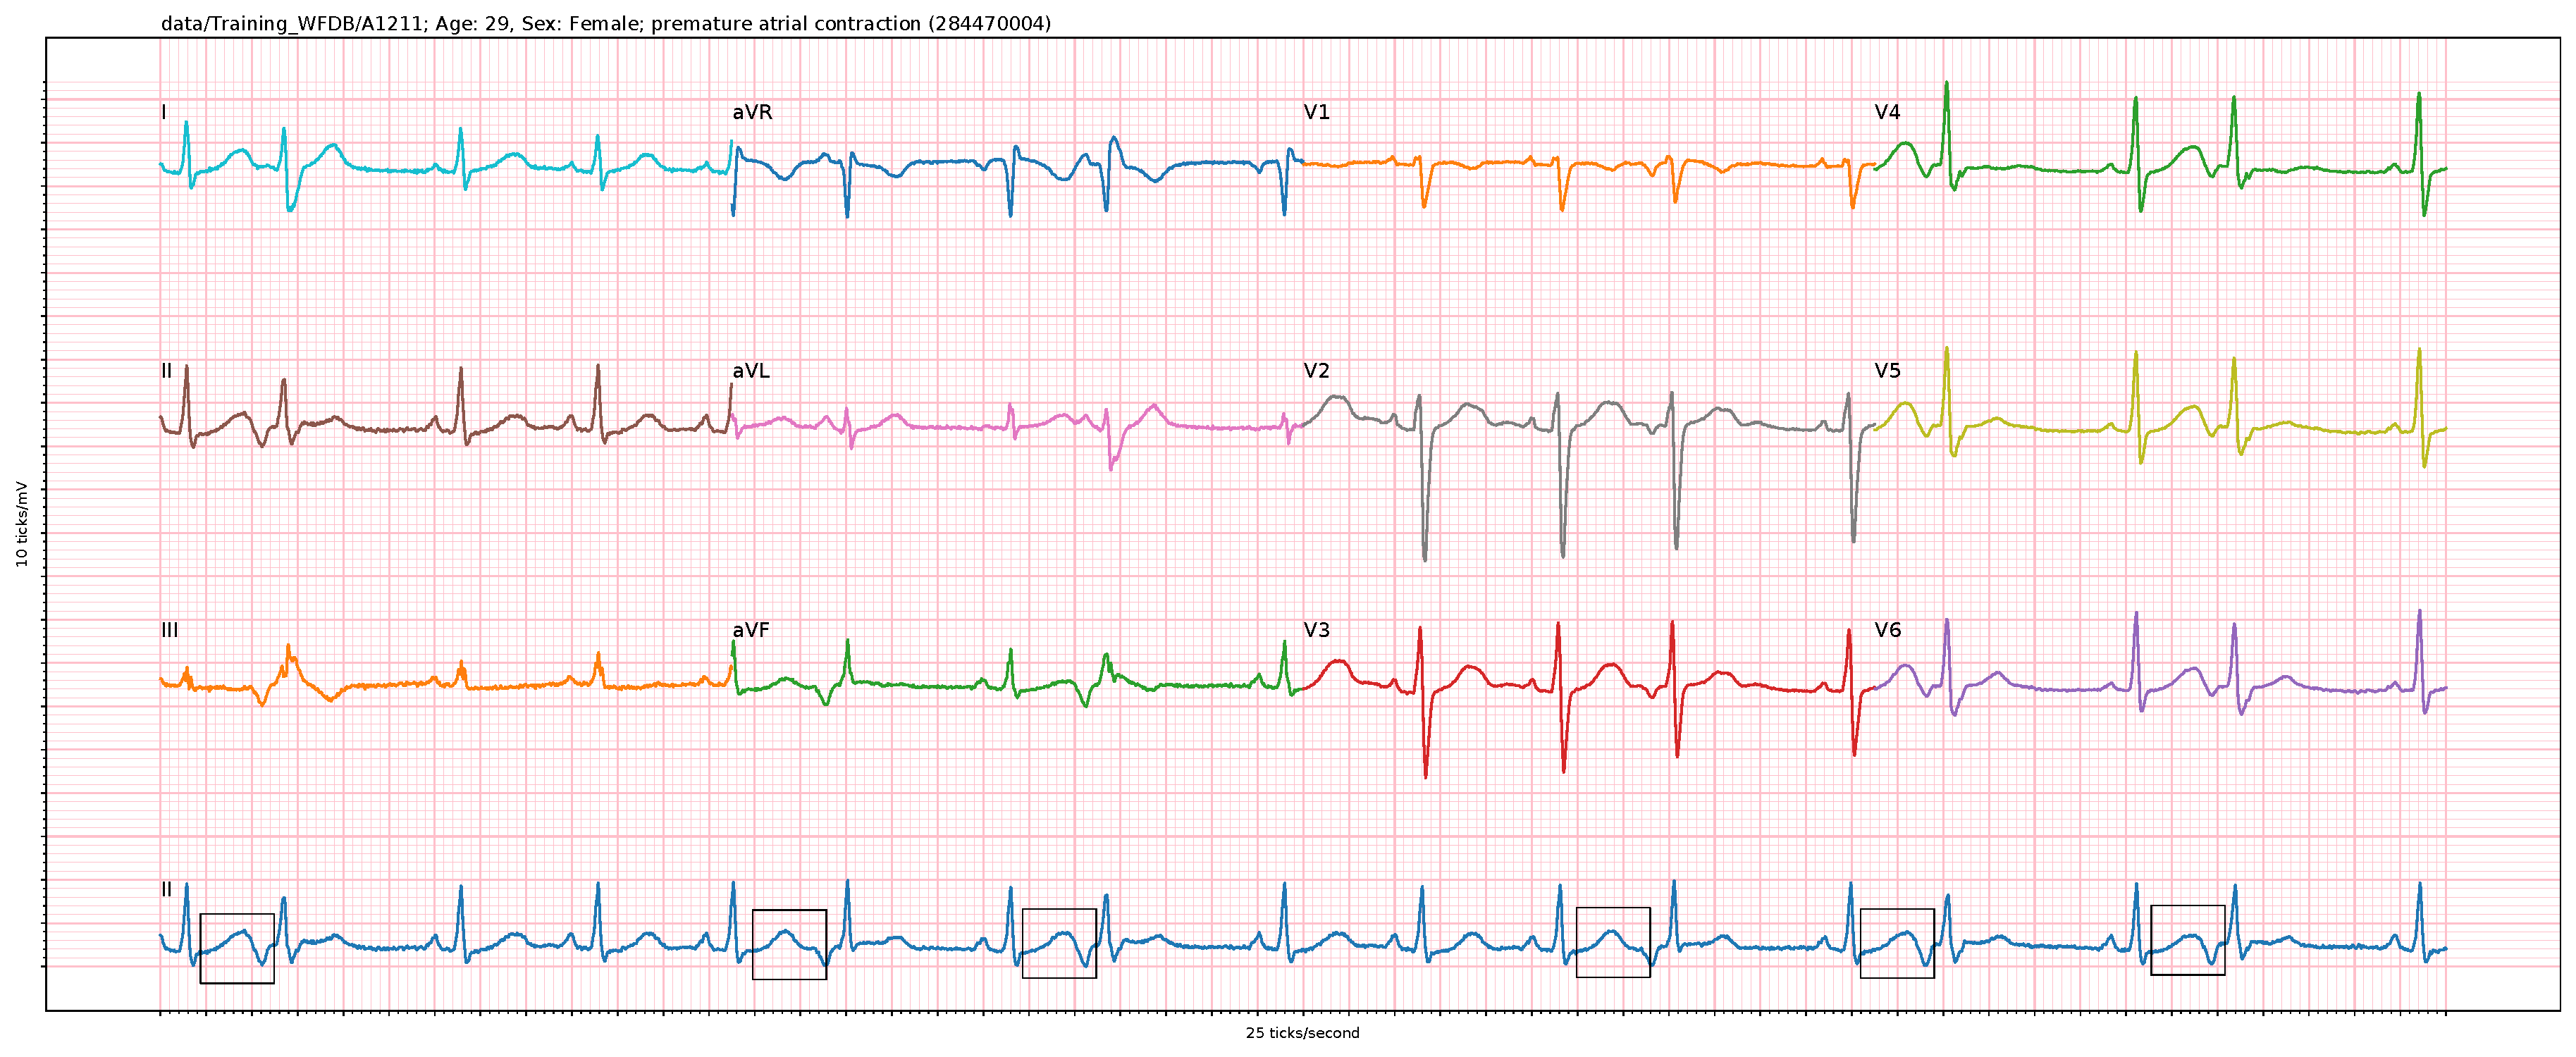
\includegraphics[width=1.2\textwidth]{figure/PAC/full_95_4661_emph.pdf}}
        \caption{Instance of 12-lead \gls{ecg} with premature atrial contraction. Instances of P waves occurring within preceding beat T wave in lead II are emphasized with black squares.}
        \label{fig:full_PAC}
    \end{figure}
    \item[\gls{pac}] These events may occur as single or repetitive events along the \gls{ecg} record and are characterized by a P wave occurring within the T wave of the preceding beat~\cite{ecg-utah-lesson}.
    An example can be found in Figure~\ref{fig:full_PAC}.
 
    \begin{figure}[H]
        \centering
        \makebox[\textwidth][c]{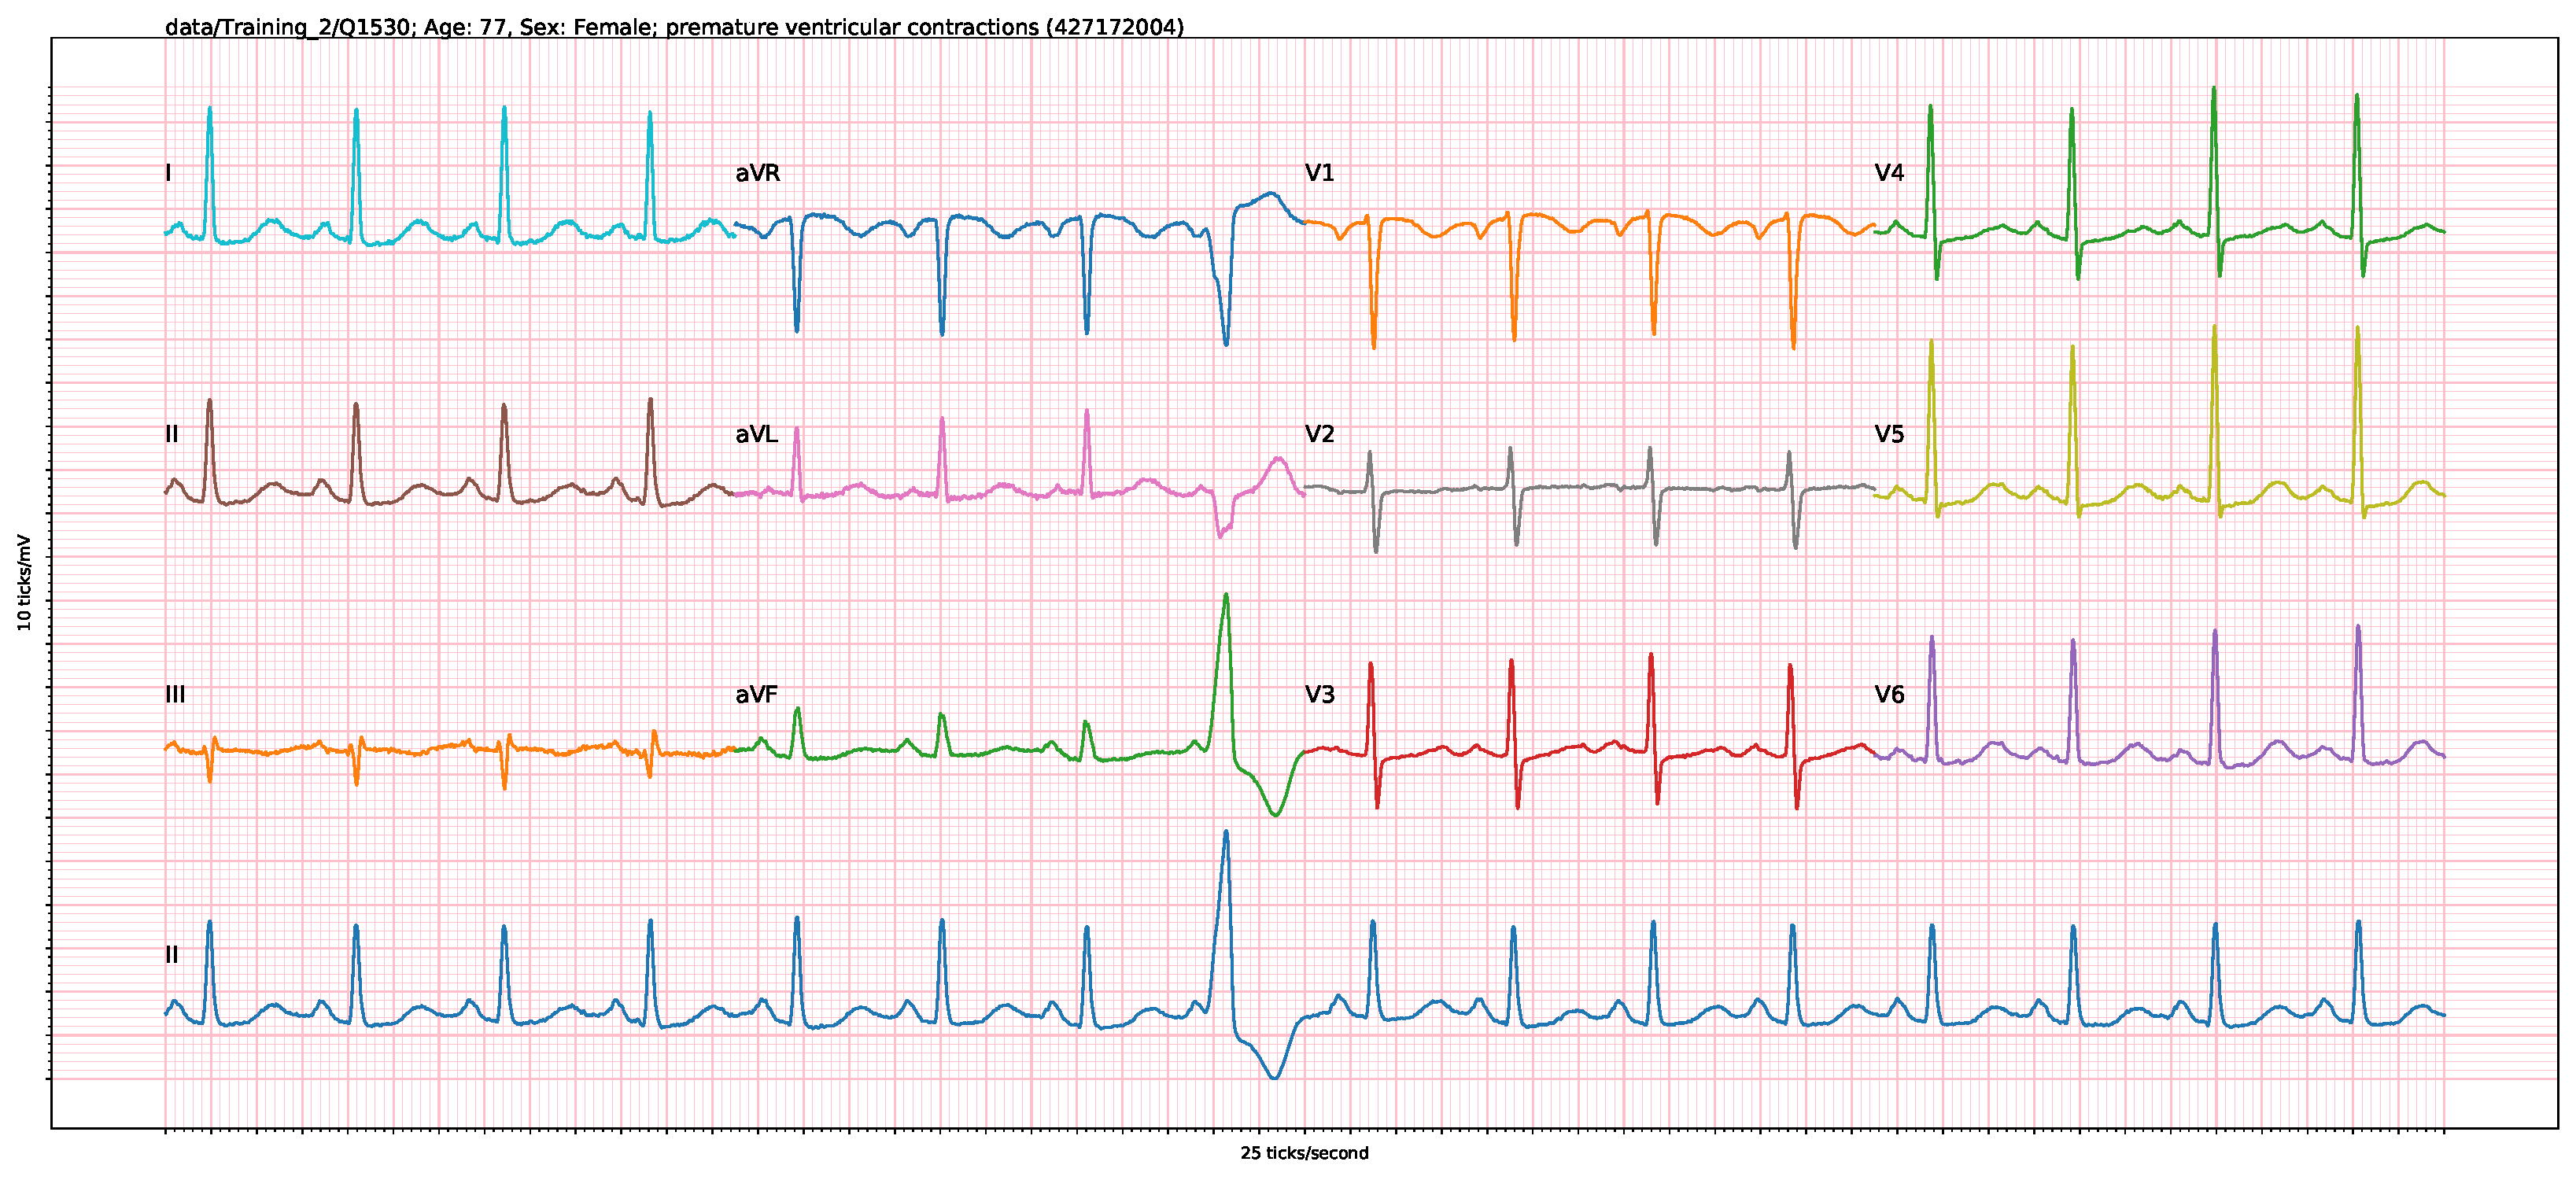
\includegraphics[width=1.2\textwidth]{figure/PVC/full_4_1478.pdf}}
        \caption{Instance of 12-lead \gls{ecg} with premature ventricular contraction. Premature ventricular contraction occurs at the 4.5 second mark.}
        \label{fig:full_PVC}
    \end{figure}
    \item[\gls{pvc}] This diagnosis indicates that a ventricular contraction has occurred before the next expected sinoatrial node action potential~\cite{surawicz_borys_ahaaccfhrs_2009}. It may occur as singular or repetitive events along the \gls{ecg} record.
    Refer to Figure~\ref{fig:full_PVC} for an example \gls{ecg} record containing this disorder.

    \begin{figure}[H]
        \centering
        \makebox[\textwidth][c]{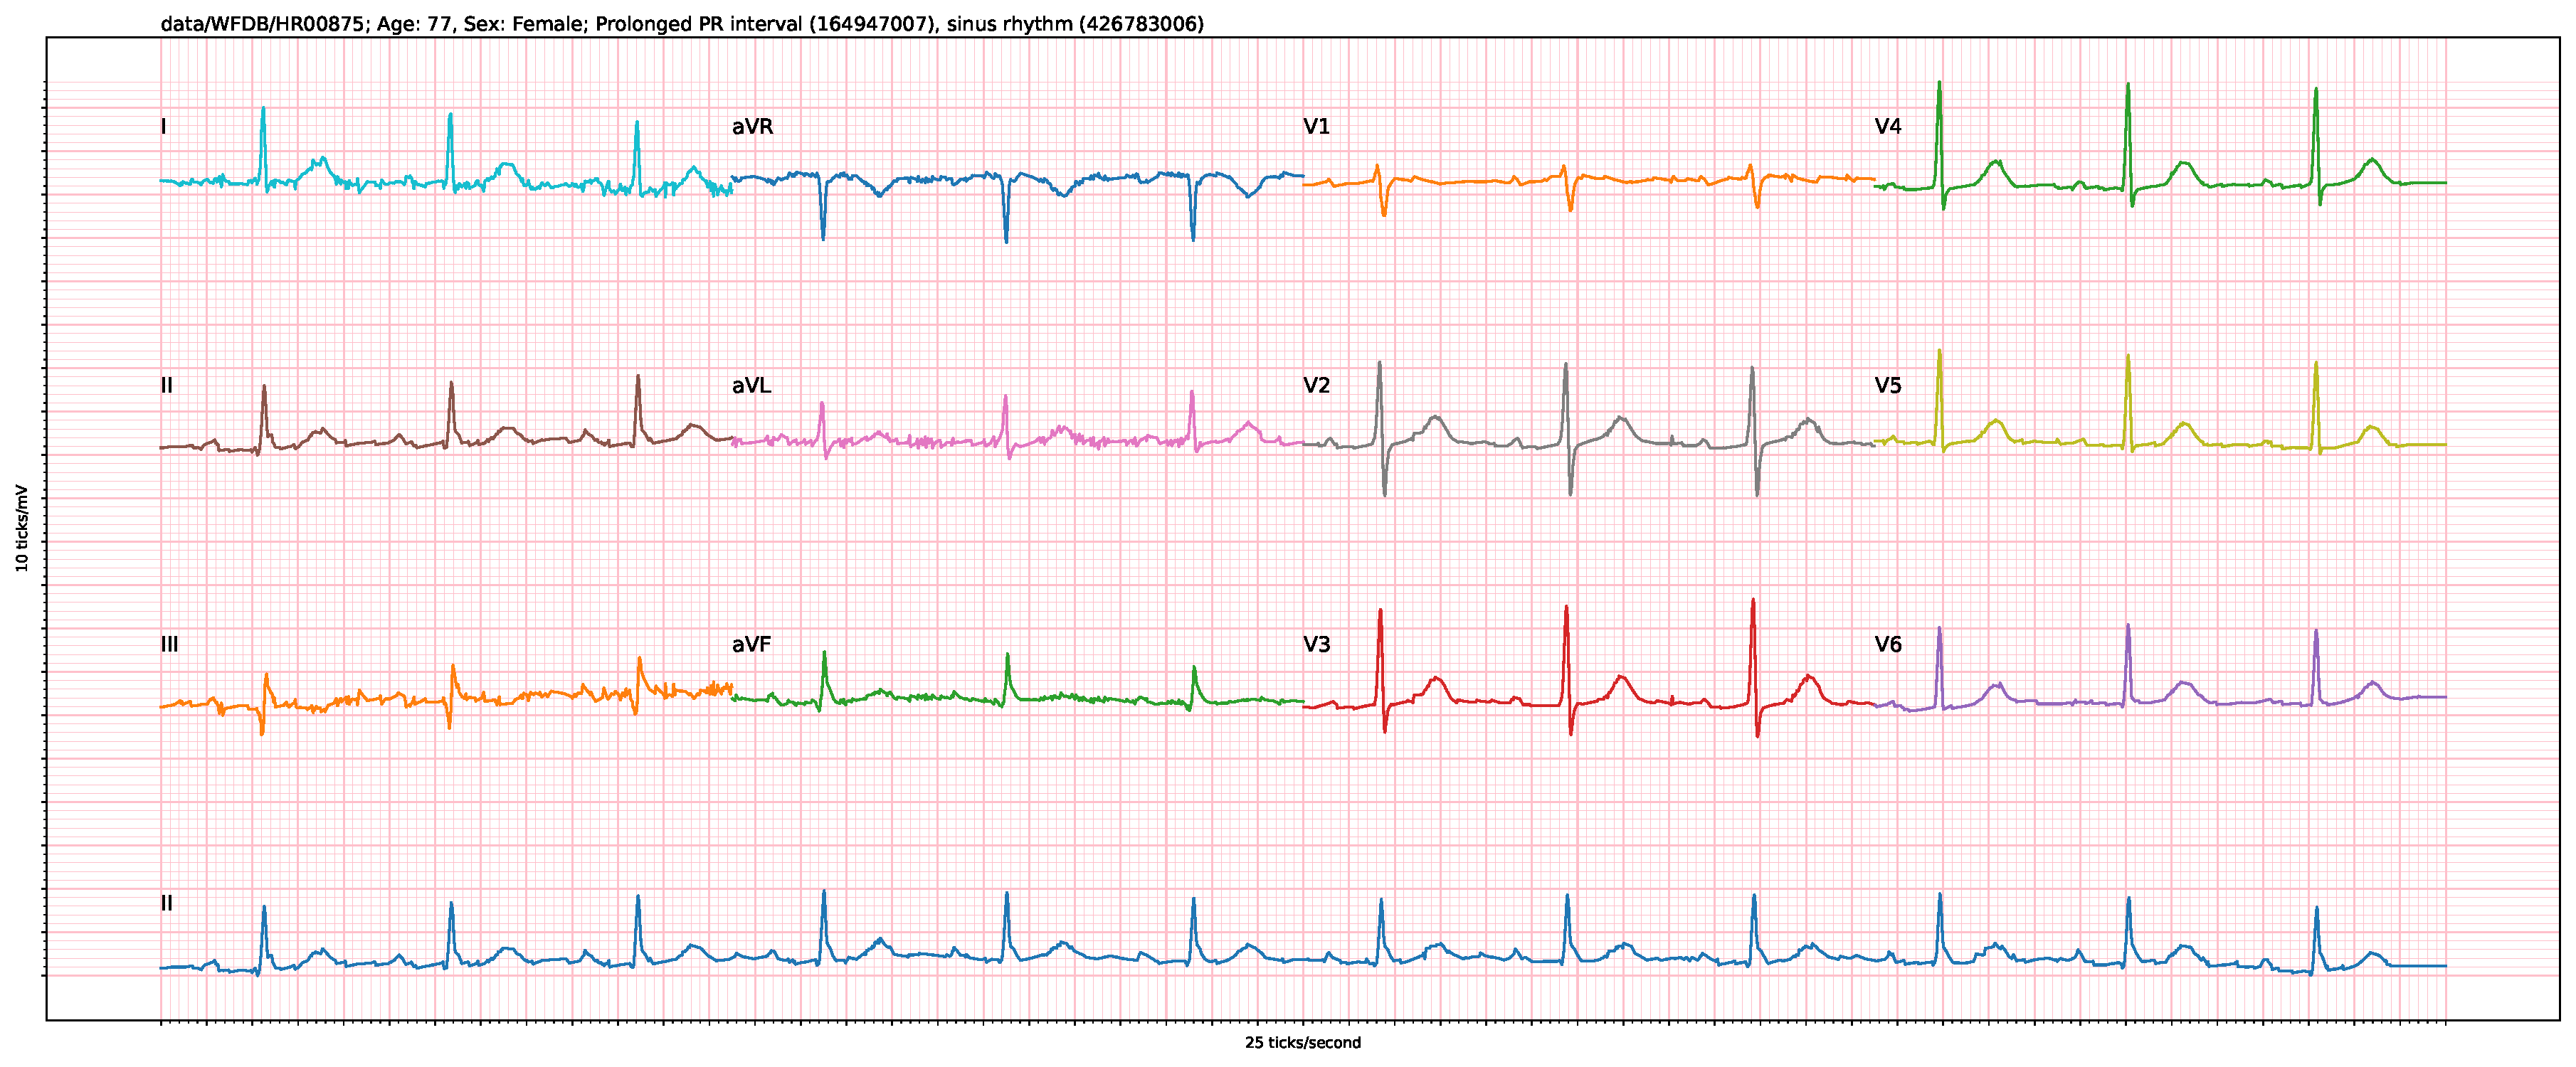
\includegraphics[width=1.2\textwidth]{figure/LPR/full_17_21546.pdf}}
        \caption{Instance of 12-lead \gls{ecg} with prolonged PR interval. Patient record contains PR intervals exceeding 200ms (5 squares) but is also diagnosed as having normal sinus rhythm.}
        \label{fig:full_LPR}
    \end{figure}
    \item[\gls{lpr}] This disorder indicates a delayed conduction through the atrioventricular node and is characterized by a PR interval exceeding 200ms~\cite{Kwok672}. This condition has overlap with \gls{iavb} but suggests reduced severity.
    An example record can be found in Figure~\ref{fig:full_LPR}.

    \begin{figure}[H]
        \centering
        \makebox[\textwidth][c]{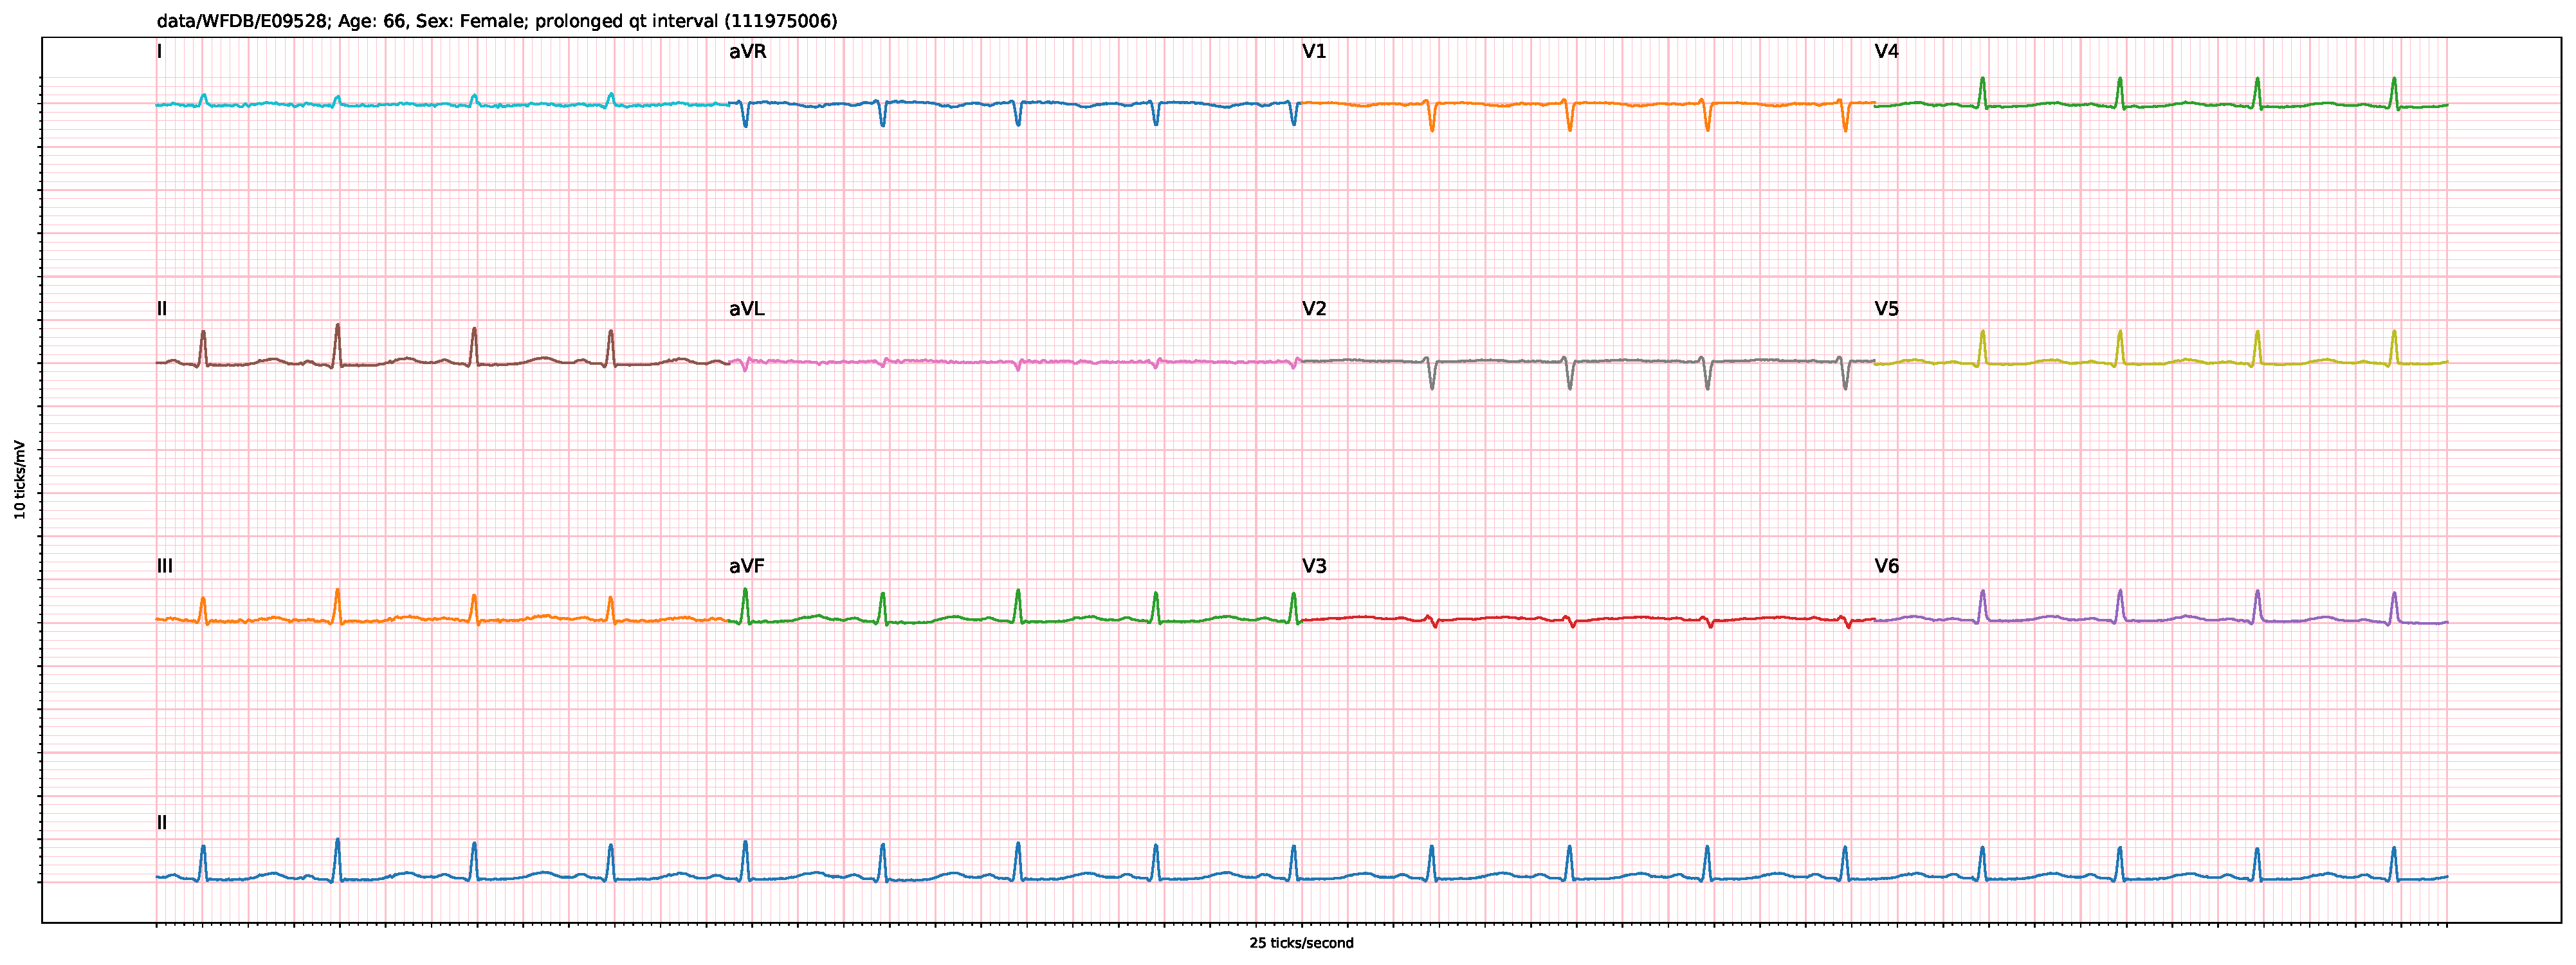
\includegraphics[width=1.2\textwidth]{figure/LQT/full_37_19855.pdf}}
        \caption{Instance of 12-lead \gls{ecg} with prolonged QT interval. Patient T waves end past the halfway point of the preceding and upcoming R peaks.}
        \label{fig:full_LQT}
    \end{figure}
    \item[\gls{lqt}] This disorder indicates that the heart is inadequately recovering after each beat and can be quickly identified by the presence of T waves ending beyond the midway point of an RR interval~\cite{10.1001/jama.1986.03380210081029}.
    See Figure~\ref{fig:full_LQT} for an example record with this disorder.

    \begin{figure}[H]
        \centering
        \makebox[\textwidth][c]{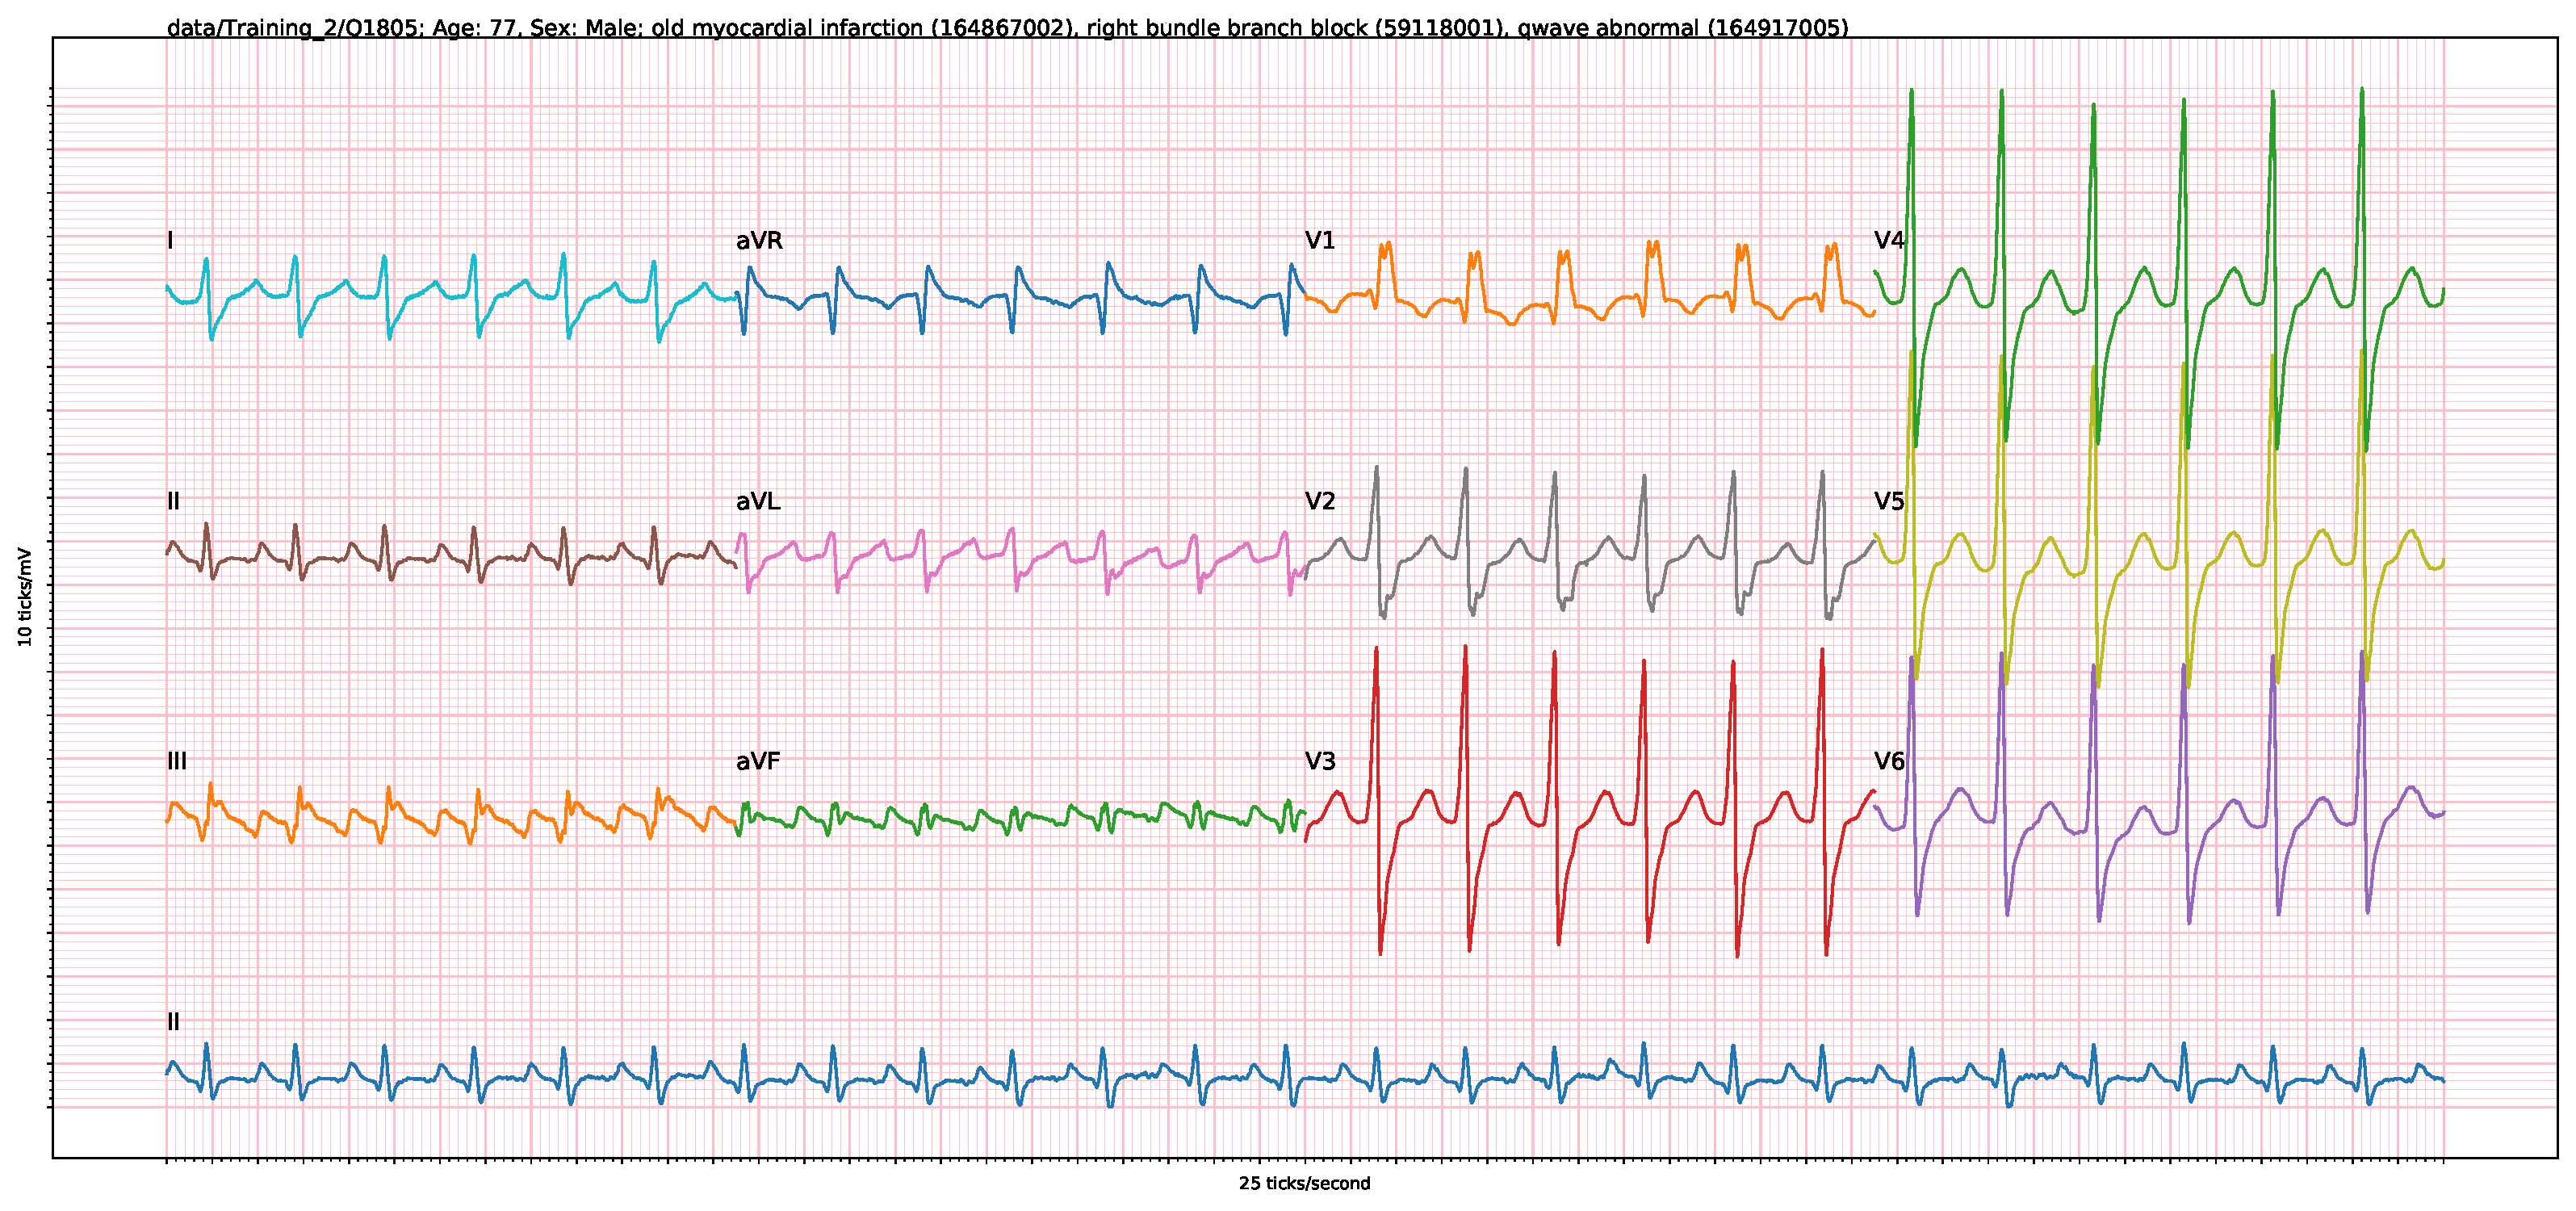
\includegraphics[width=1.2\textwidth]{figure/QAb/full_0_1740.pdf}}
        \caption{Instance of 12-lead \gls{ecg} with abnormal Q wave. Patient Q waves exceed 40ms wave duration in leads I, III, aVR, aVL, V2, V3, V4, V5, V6 and have Q wave amplutides exceeding 25\% of the QRS complex amplitude in precordial leads V2-V6.}
        \label{fig:full_QAb}
    \end{figure}
    \item[\gls{qab}]Pathologic Q waves indicate the presence of an old myocardial infarction and are diagnosed as having Q wave duration exceeding 40 ms or Q wave amplitude exceeding 25\% of the amplitude of the QRS complex~\cite{doi:10.1002/clc.4960200515}.
    Figure~\ref{fig:full_QAb} showcases an example record containing abnormal Q wave.

    \begin{figure}[H]
        \centering
        \makebox[\textwidth][c]{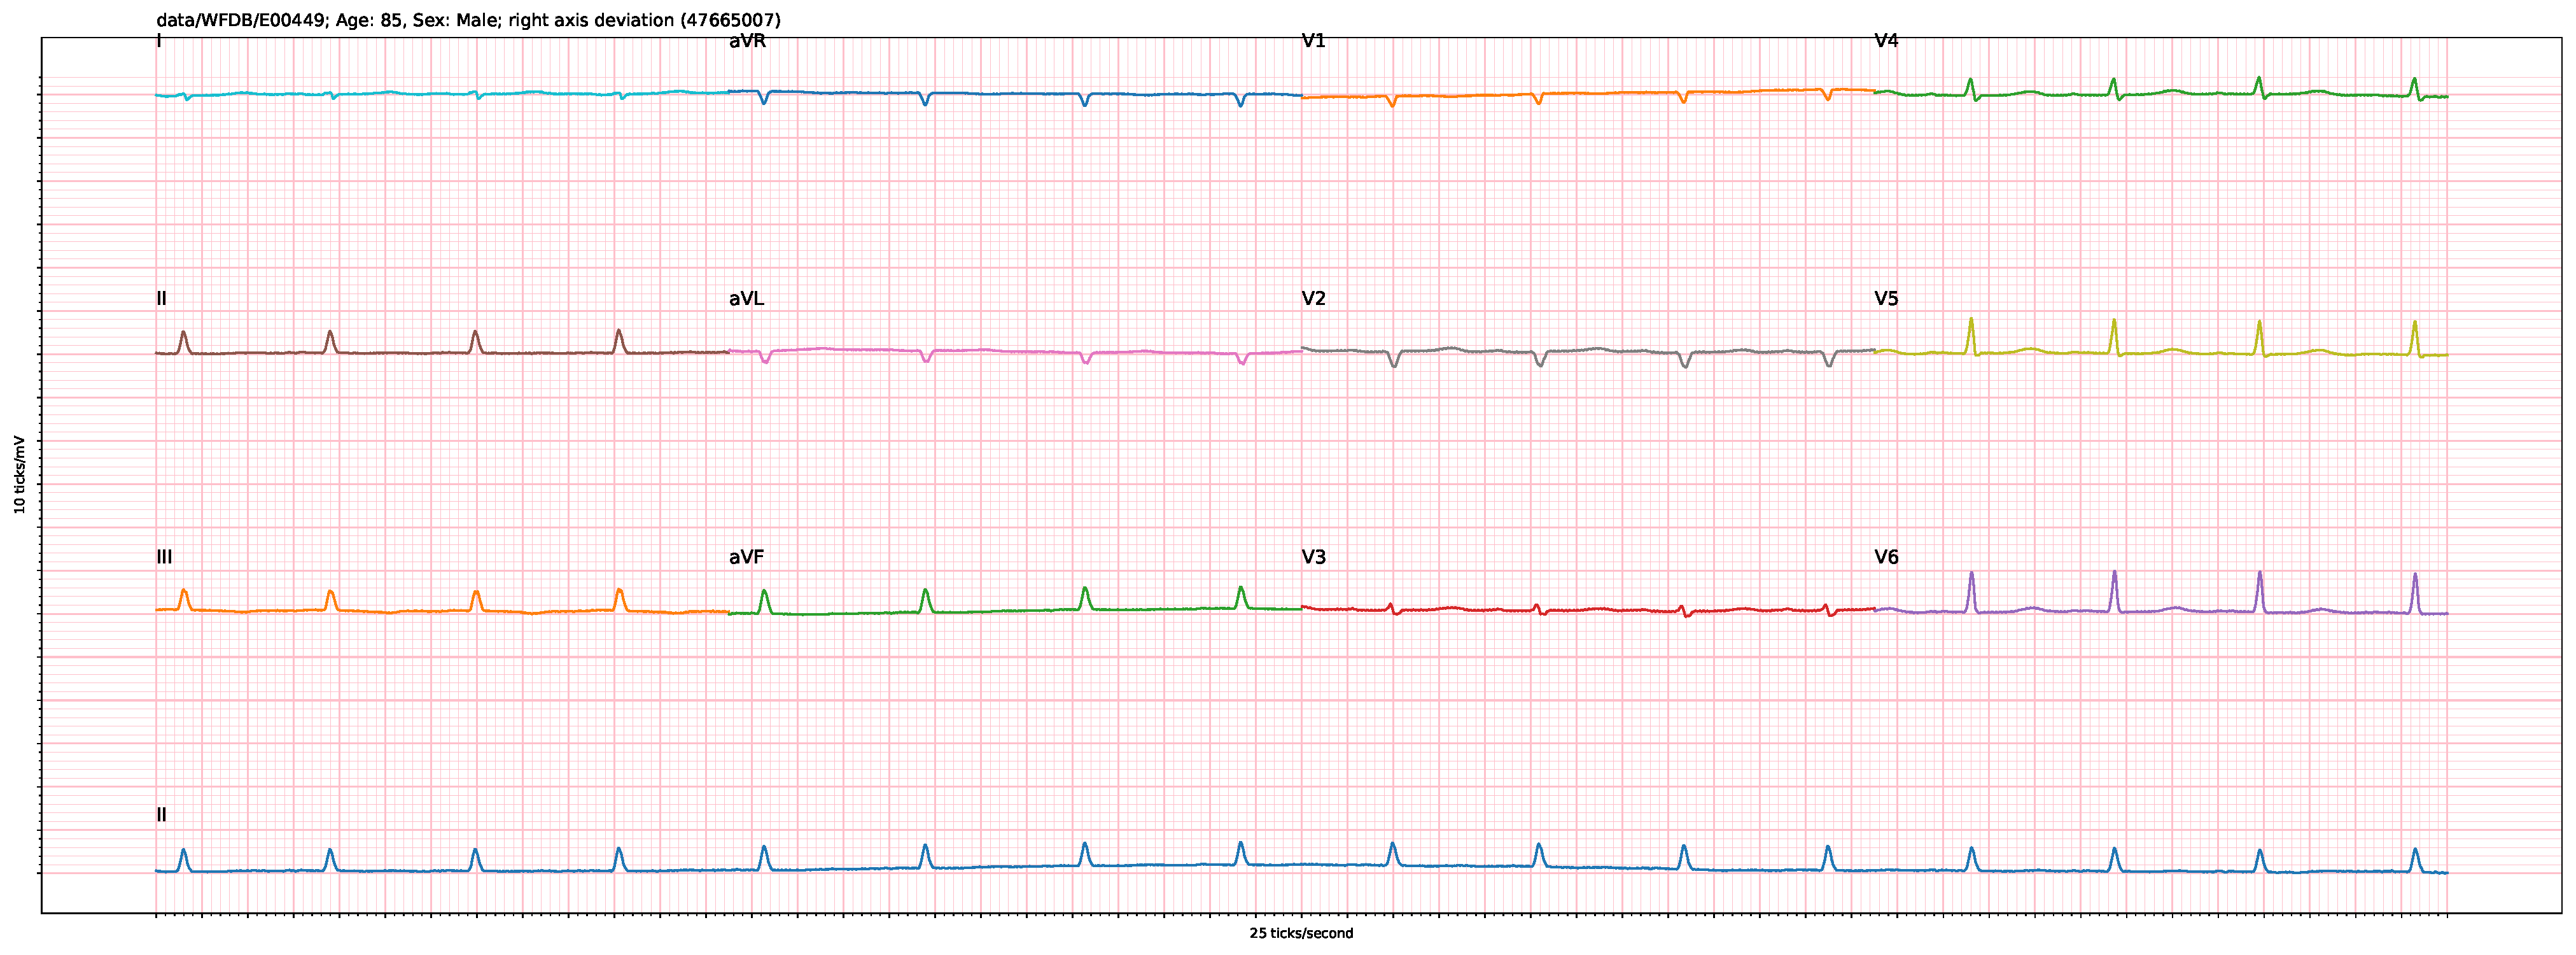
\includegraphics[width=1.2\textwidth]{figure/RAD/full_0_10776.pdf}}
        \caption{Instance of 12-lead \gls{ecg} with right axis deviation. A negative lead I with positive leads II and III suggest right axis deviation. Using the hexaxial system, leads II, III, and aVF all have the largest QRS amplitudes (each approximately 0.3mV), resulting in an cardiac axis estimate between $60\degree$ and $120\degree$. This overlaps with our right axis deviation criteria where the axis exists between $90\degree$ and $180\degree$.}
        \label{fig:full_RAD}
    \end{figure}
    \item[\gls{rad}] This diagnosis indicates the cardiac axis existing between $90\degree$ and $180\degree$. See Figure~\ref{fig:full_RAD} for an example ECG record interpreted using the lead I, II, III approach as well as the hexaxial reference system.

    \item[\gls{rbbb}] This diagnosis is identical to \gls{crbbb}.

    \begin{figure}[H]
        \centering
        \makebox[\textwidth][c]{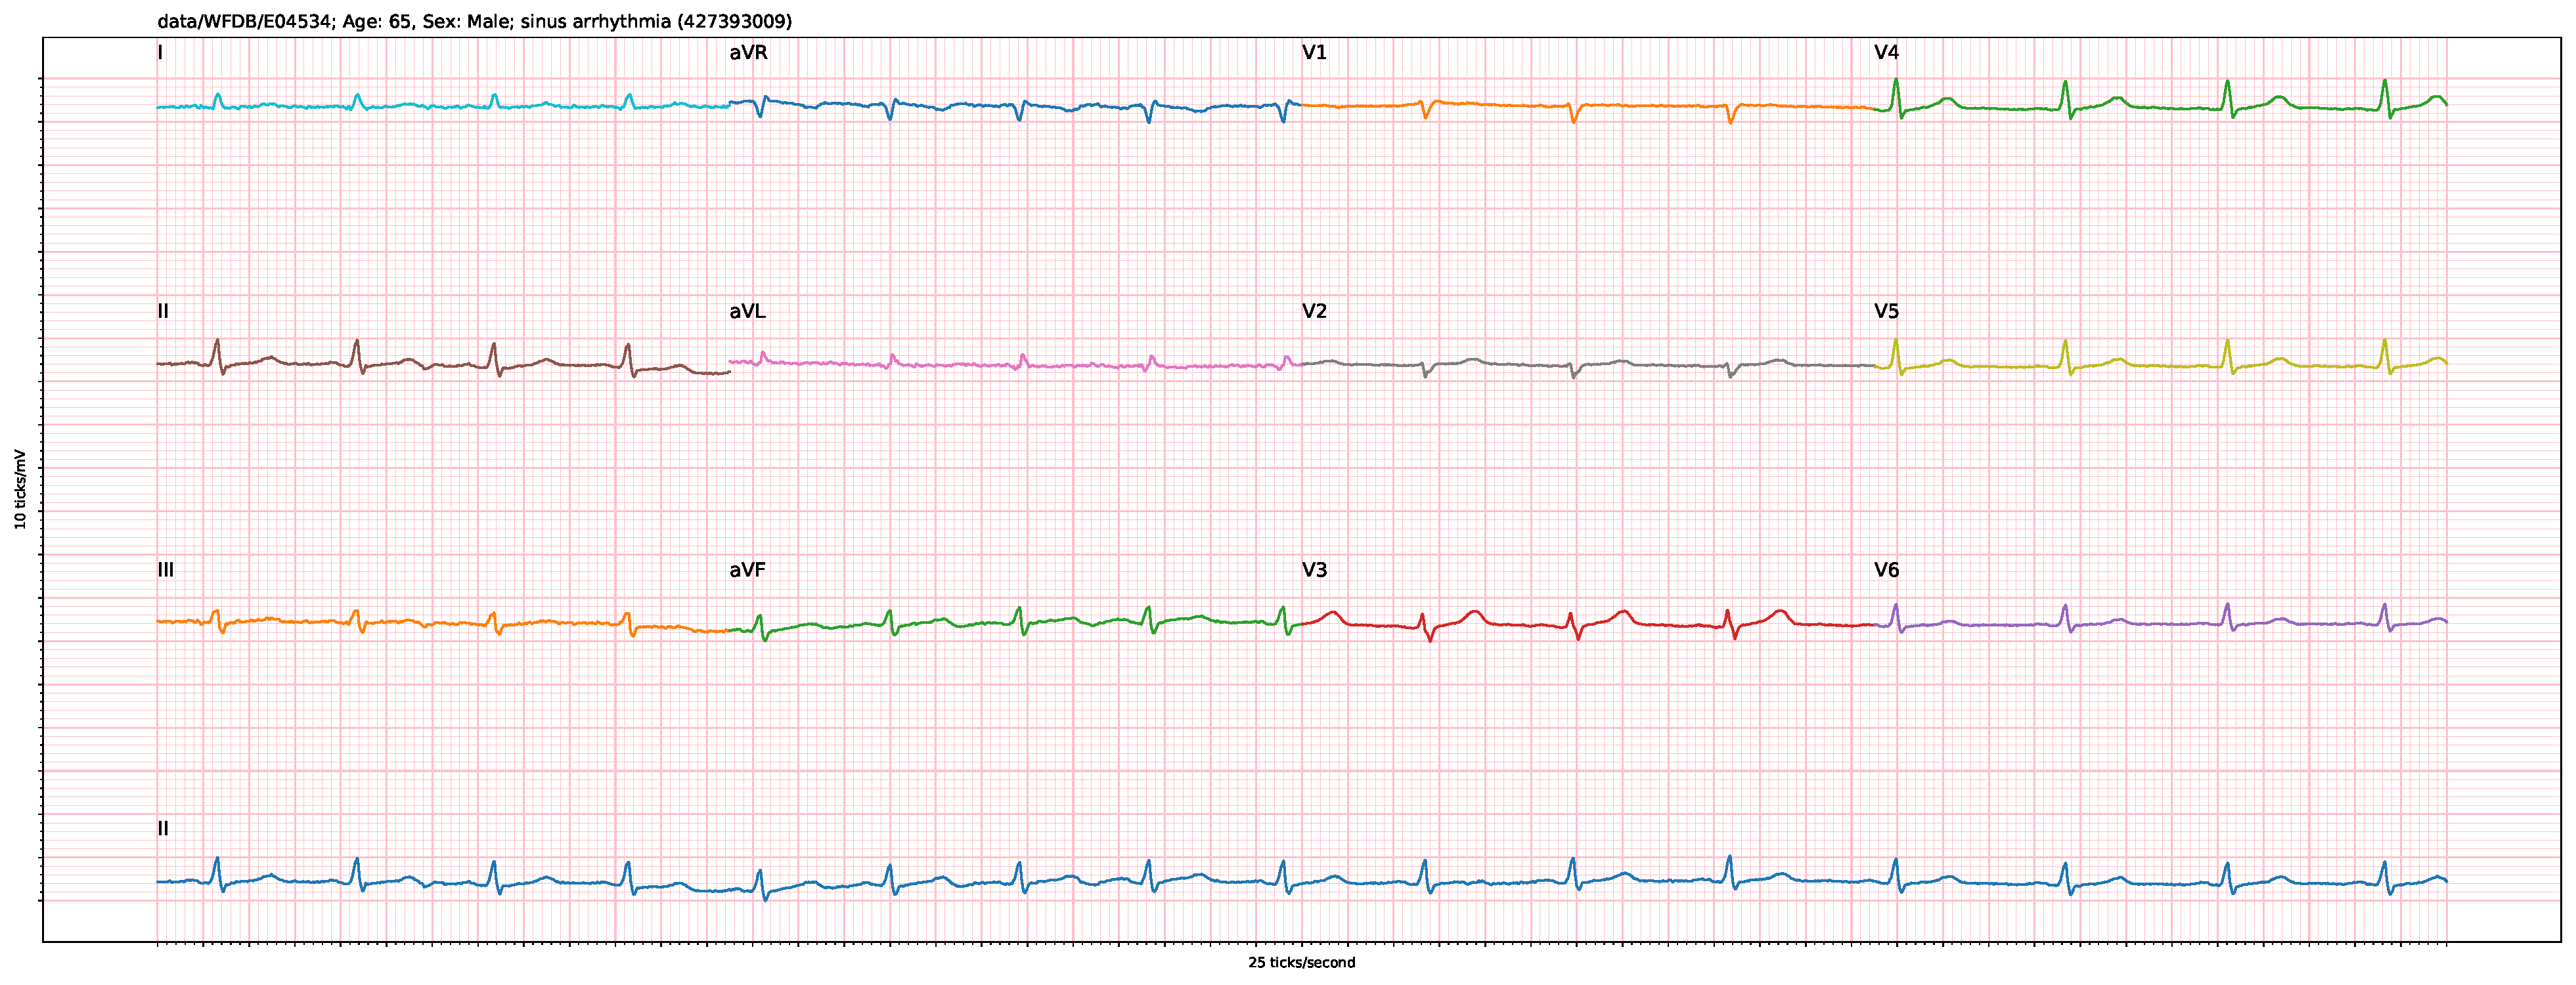
\includegraphics[width=1.2\textwidth]{figure/SA/full_37_14861.pdf}}
        \caption{Instance of 12-lead \gls{ecg} with sinus arrhythmia. Recorded heart rate decreases over time, or distance between R peaks increases over time.}
        \label{fig:full_SA}
    \end{figure}
    \item[\gls{sa}] This diagnosis reflects a change in the beat-to-beat variation over time, resulting in an irregular heart rate~\cite{surawicz_borys_ahaaccfhrs_2009}.
    This condition is typically not serious.
    An example of an \gls{ecg} record with \gls{sa} can be found in Figure~\ref{fig:full_SA}.

    \begin{figure}[H]
        \centering
        \makebox[\textwidth][c]{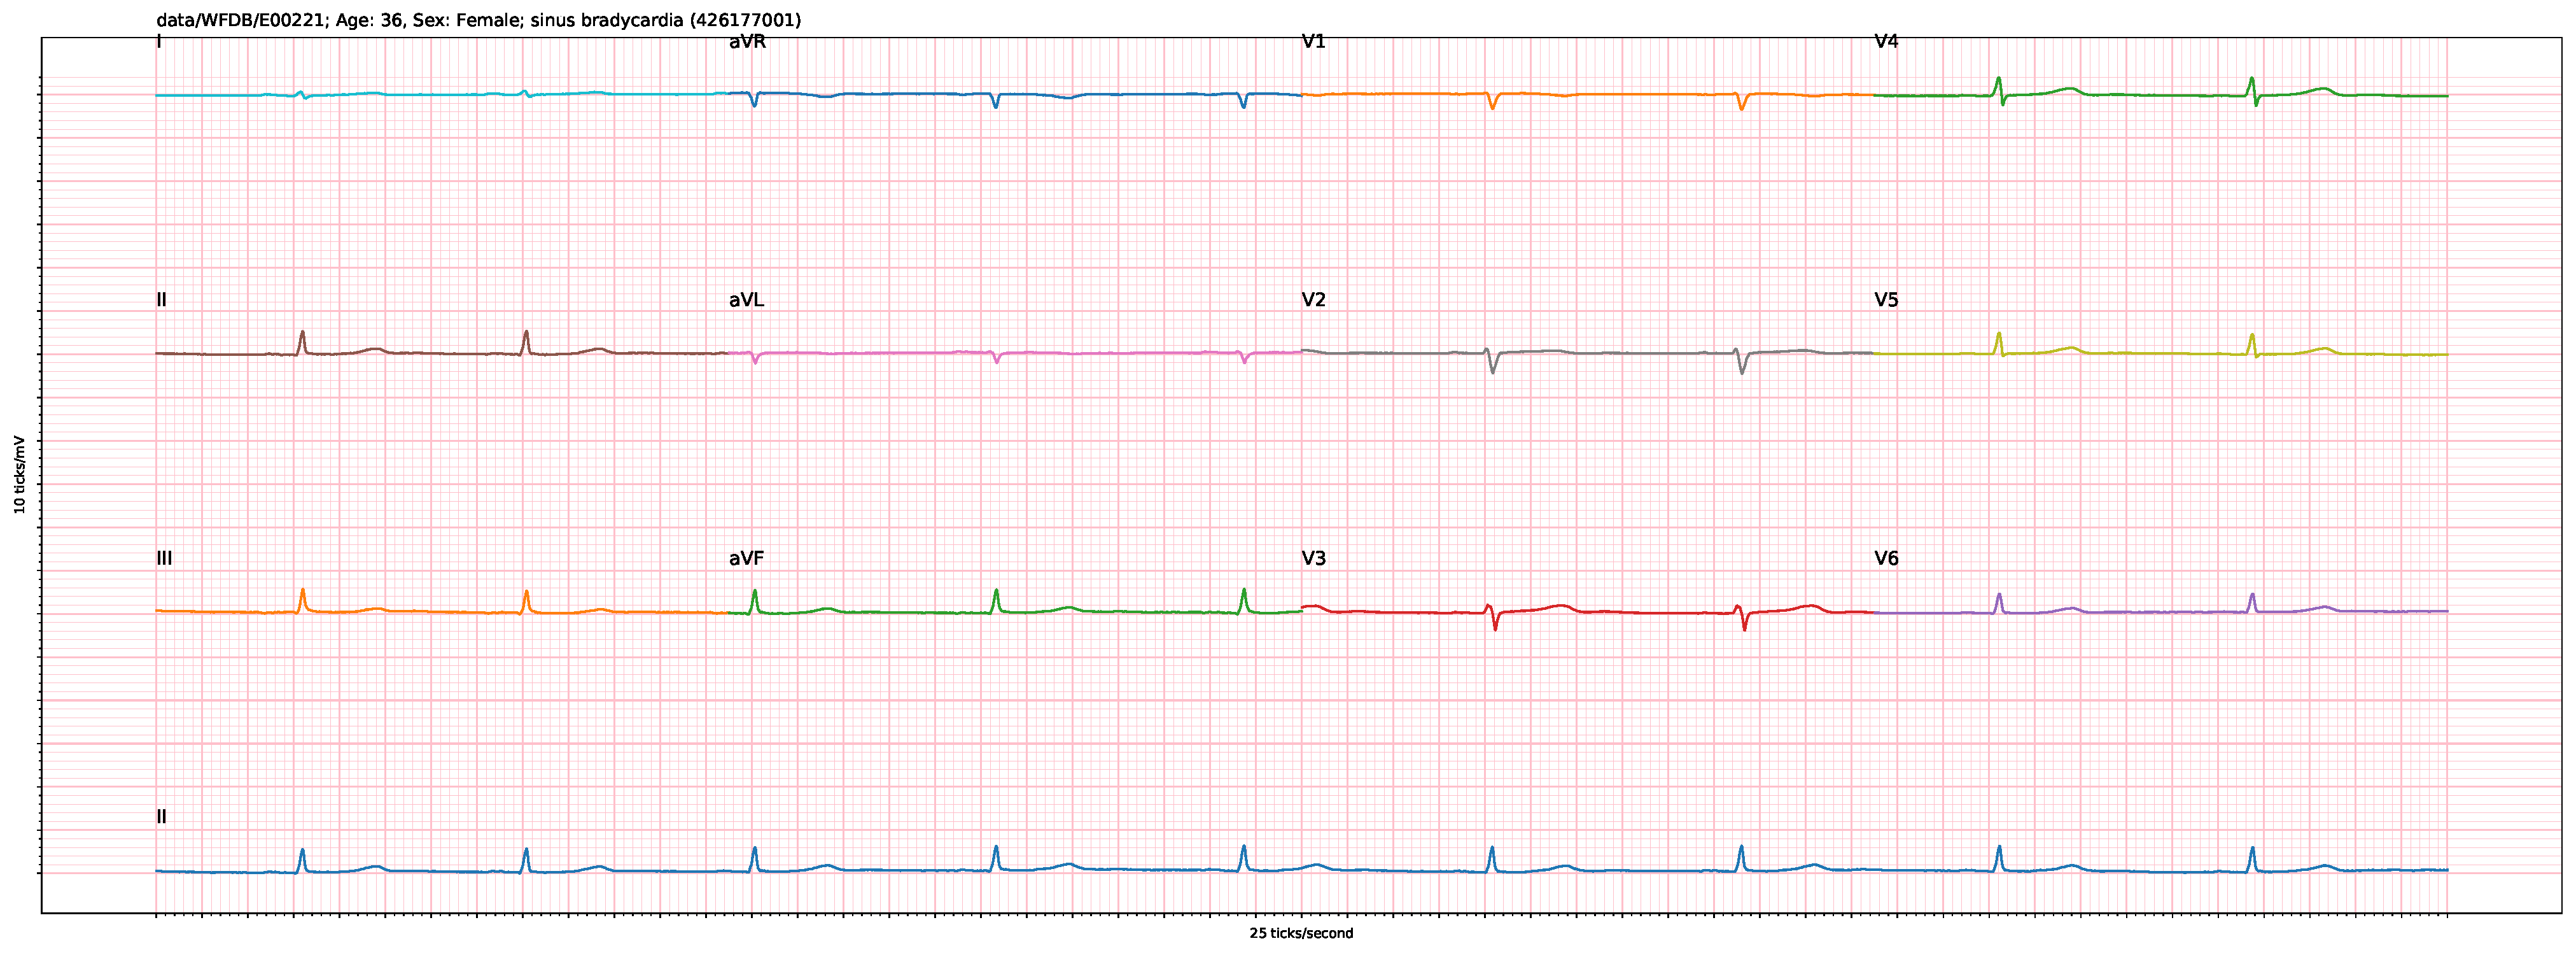
\includegraphics[width=1.2\textwidth]{figure/SB/full_6_10548.pdf}}
        \caption{Instance of 12-lead \gls{ecg} with sinus bradycardia. Upright P wave in lead II exists, with a mean heart rate of 59 beats per minute.}
        \label{fig:full_SB}
    \end{figure}
    \item[\gls{sb}] This specific type of slow heartbeat is caused by the sinoatrial node firing less than 60 times per minute.
    It is characterized by an upright P wave in lead II preceding every QRS complex and a heart rate of less than 60 beats per minute in adults.
    An example record is shown in Figure~\ref{fig:full_SB}.

    \begin{figure}[H]
        \centering
        \makebox[\textwidth][c]{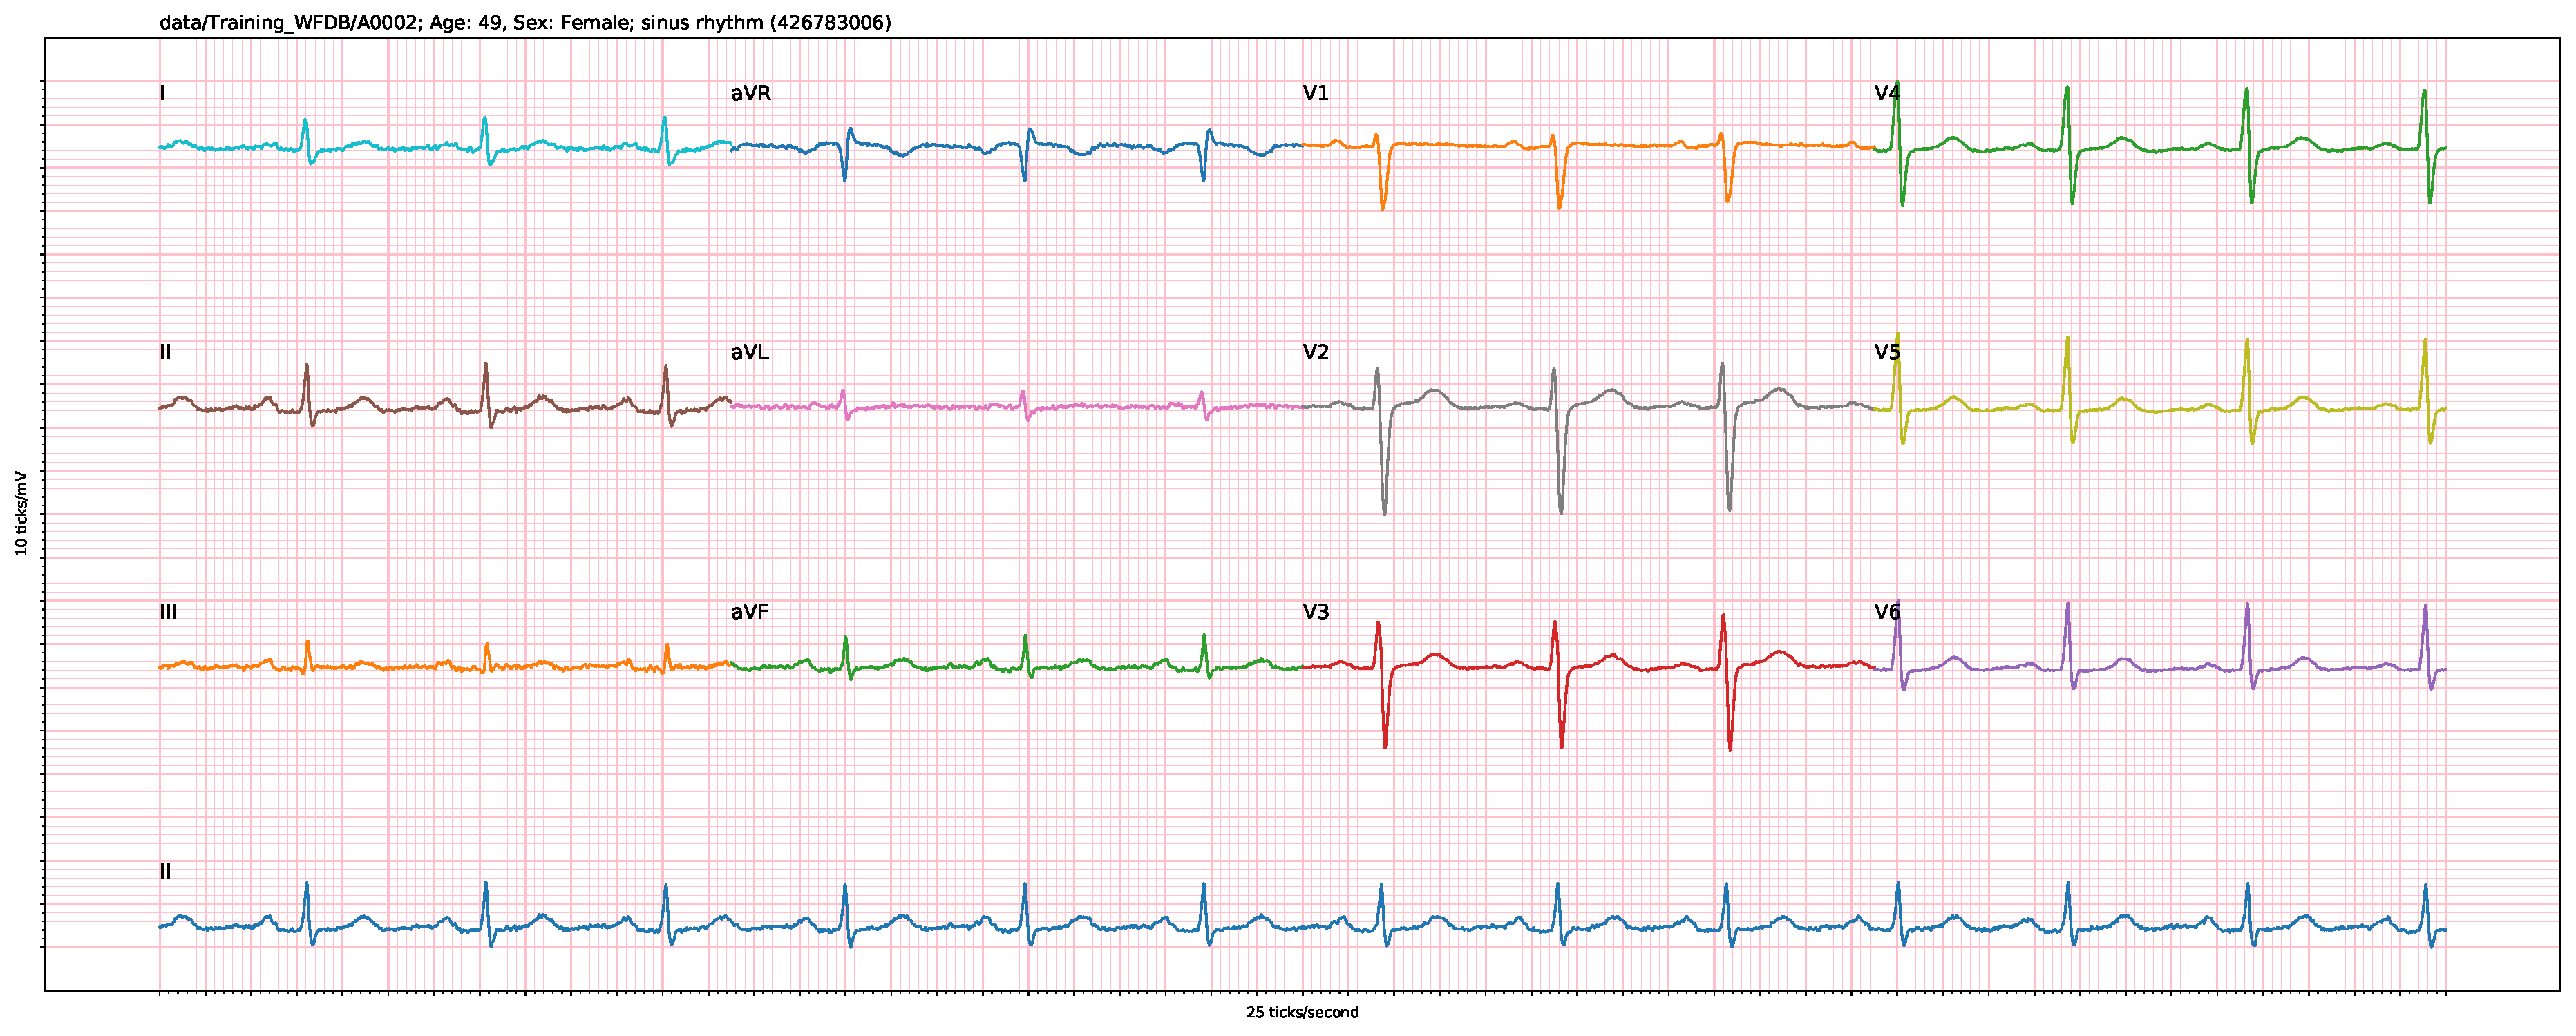
\includegraphics[width=1.2\textwidth]{figure/SNR/full_0_3452.pdf}}
        \caption{Instance of 12-lead \gls{ecg} with normal sinus rhythm. No visible defects or abnormalities indicated.}
        \label{fig:full_SNR}
    \end{figure}
    \item[\gls{snr}] The normal, healthy case for an \gls{ecg} record must have an upright P wave in leads I and II, with a QRS complex following each P wave~\cite{meek_introduction_2002}. In an adult, the resting heart rate should be between 60-99 beats per minute.
    A reference \gls{ecg} can be found in Figure~\ref{fig:full_SNR}

    \begin{figure}[H]
        \centering
        \makebox[\textwidth][c]{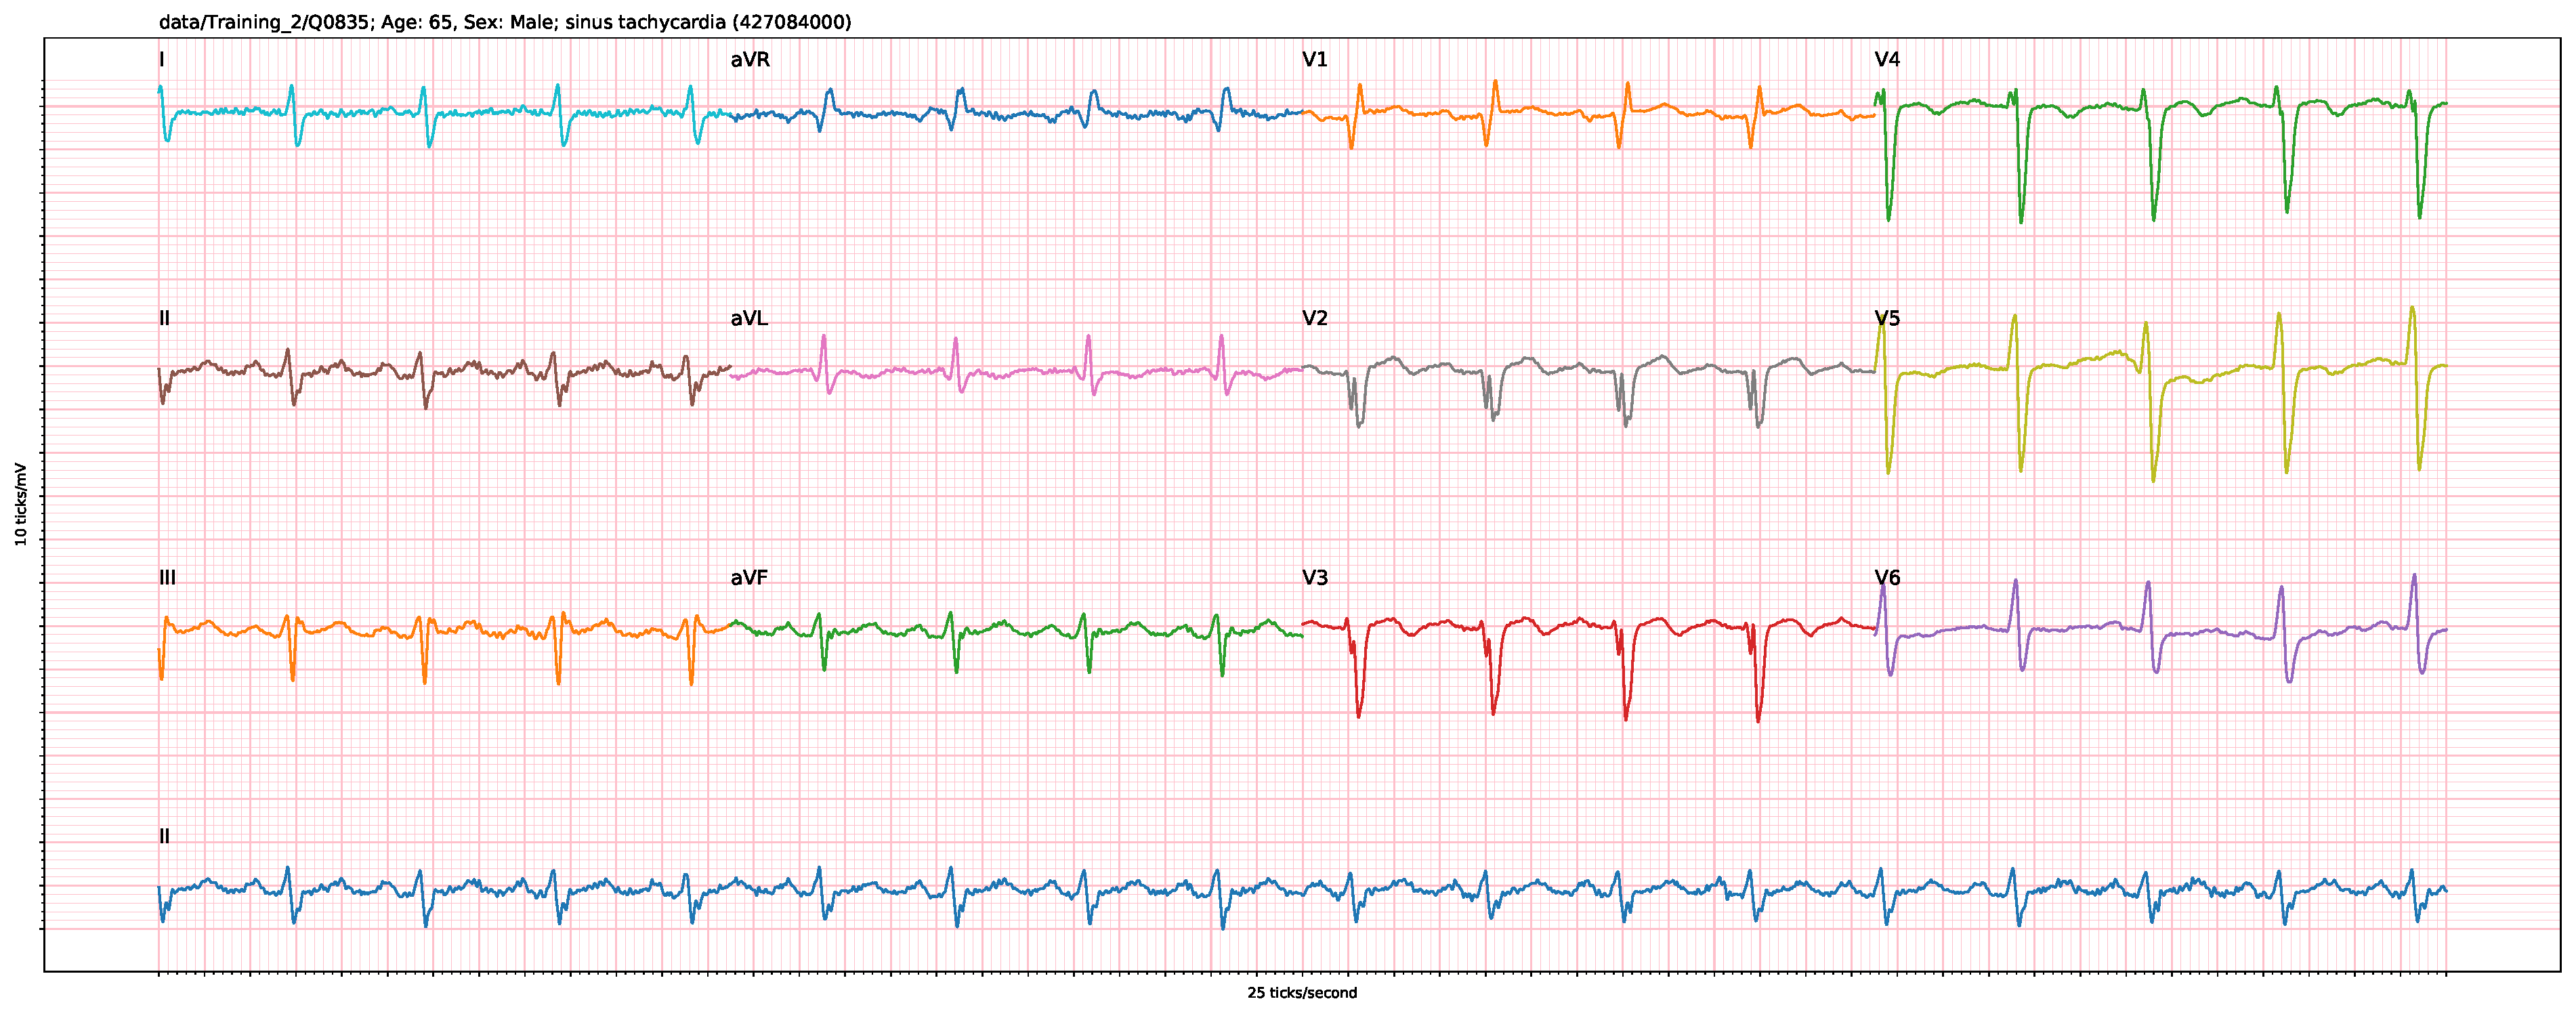
\includegraphics[width=1.2\textwidth]{figure/STach/full_0_807.pdf}}
        \caption{Instance of 12-lead \gls{ecg} with sinus tachycardia. The average heart rate is 101 beats per minute.}
        \label{fig:full_STach}
    \end{figure}
    \item[\gls{stach}] This is when the resting heart rate exceeds 100 beats per minute in adults, or above the normal range relative to the patient age.
    An example \gls{ecg} record is shown in Figure~\ref{fig:full_STach}

    \begin{figure}[H]
        \centering
        \makebox[\textwidth][c]{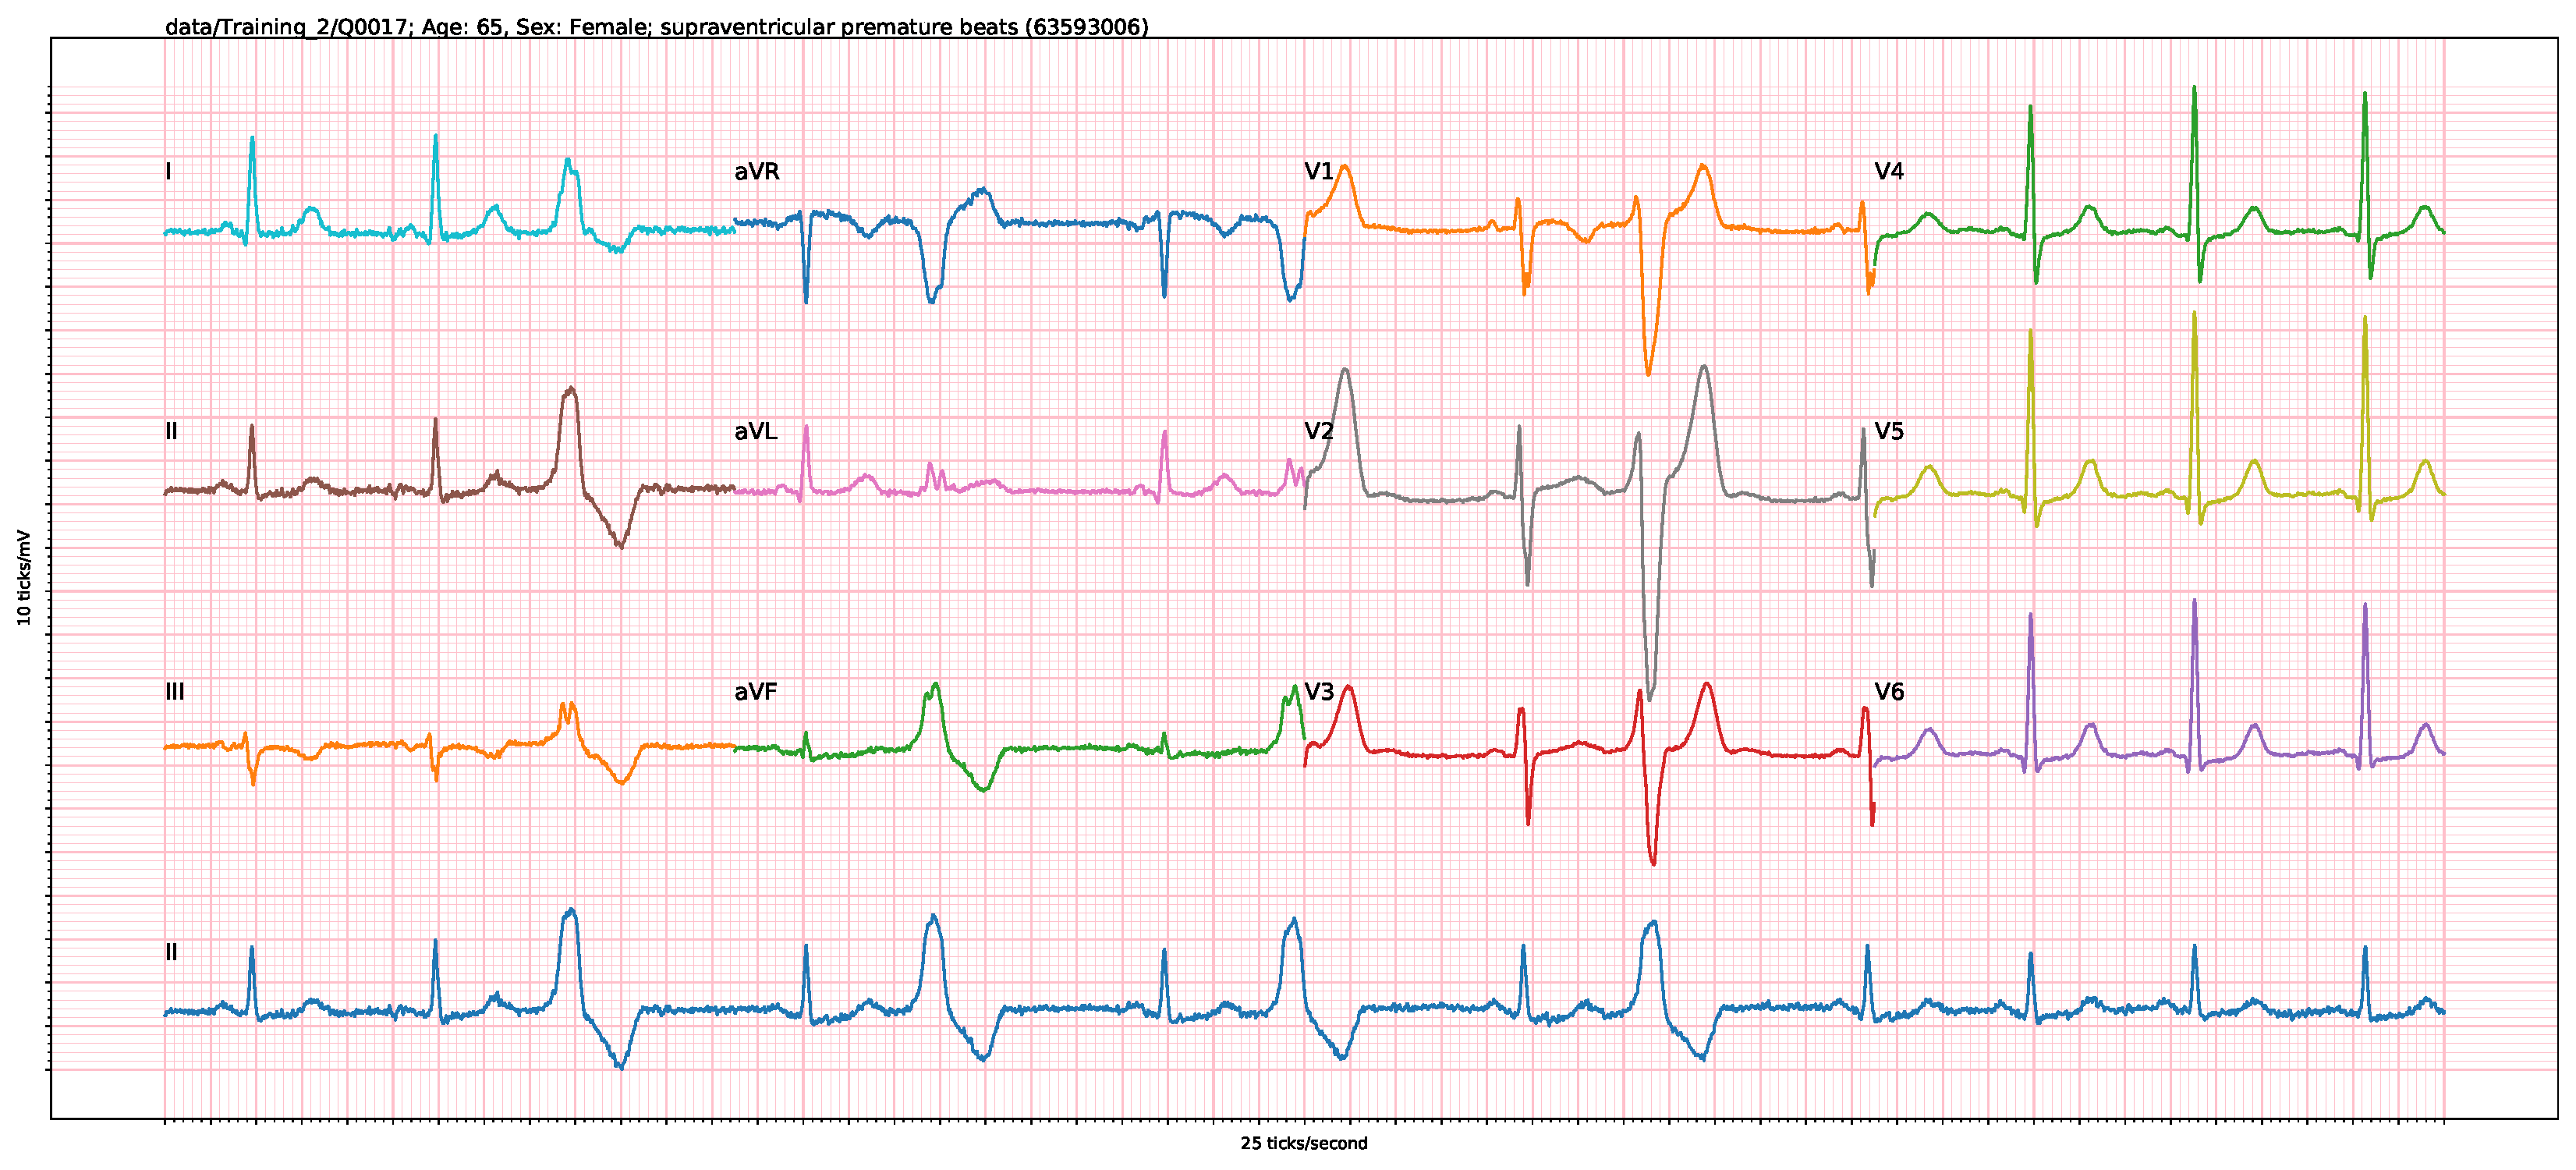
\includegraphics[width=1.2\textwidth]{figure/SVPB/full_0_14.pdf}}
        \caption{Instance of 12-lead \gls{ecg} with supraventricular premature beats. Four instances of premature ventricular beats are observed in this record.}
        \label{fig:full_SVPB}
    \end{figure}
    \item[\gls{svpb}] This occurs when the atrial contractions are triggered through invalid conduction such as an origin other than the sinoatrial node~\cite{GOLDBERGER2018130}.
    See Figure~\ref{fig:full_SVPB} for a reference \gls{ecg} with this disorder.
    For the PhysioNet challenge, this diagnosis is treated identically to \gls{pac}, despite different \gls{ecg} characteristics.

    \begin{figure}[H]
        \centering
        \makebox[\textwidth][c]{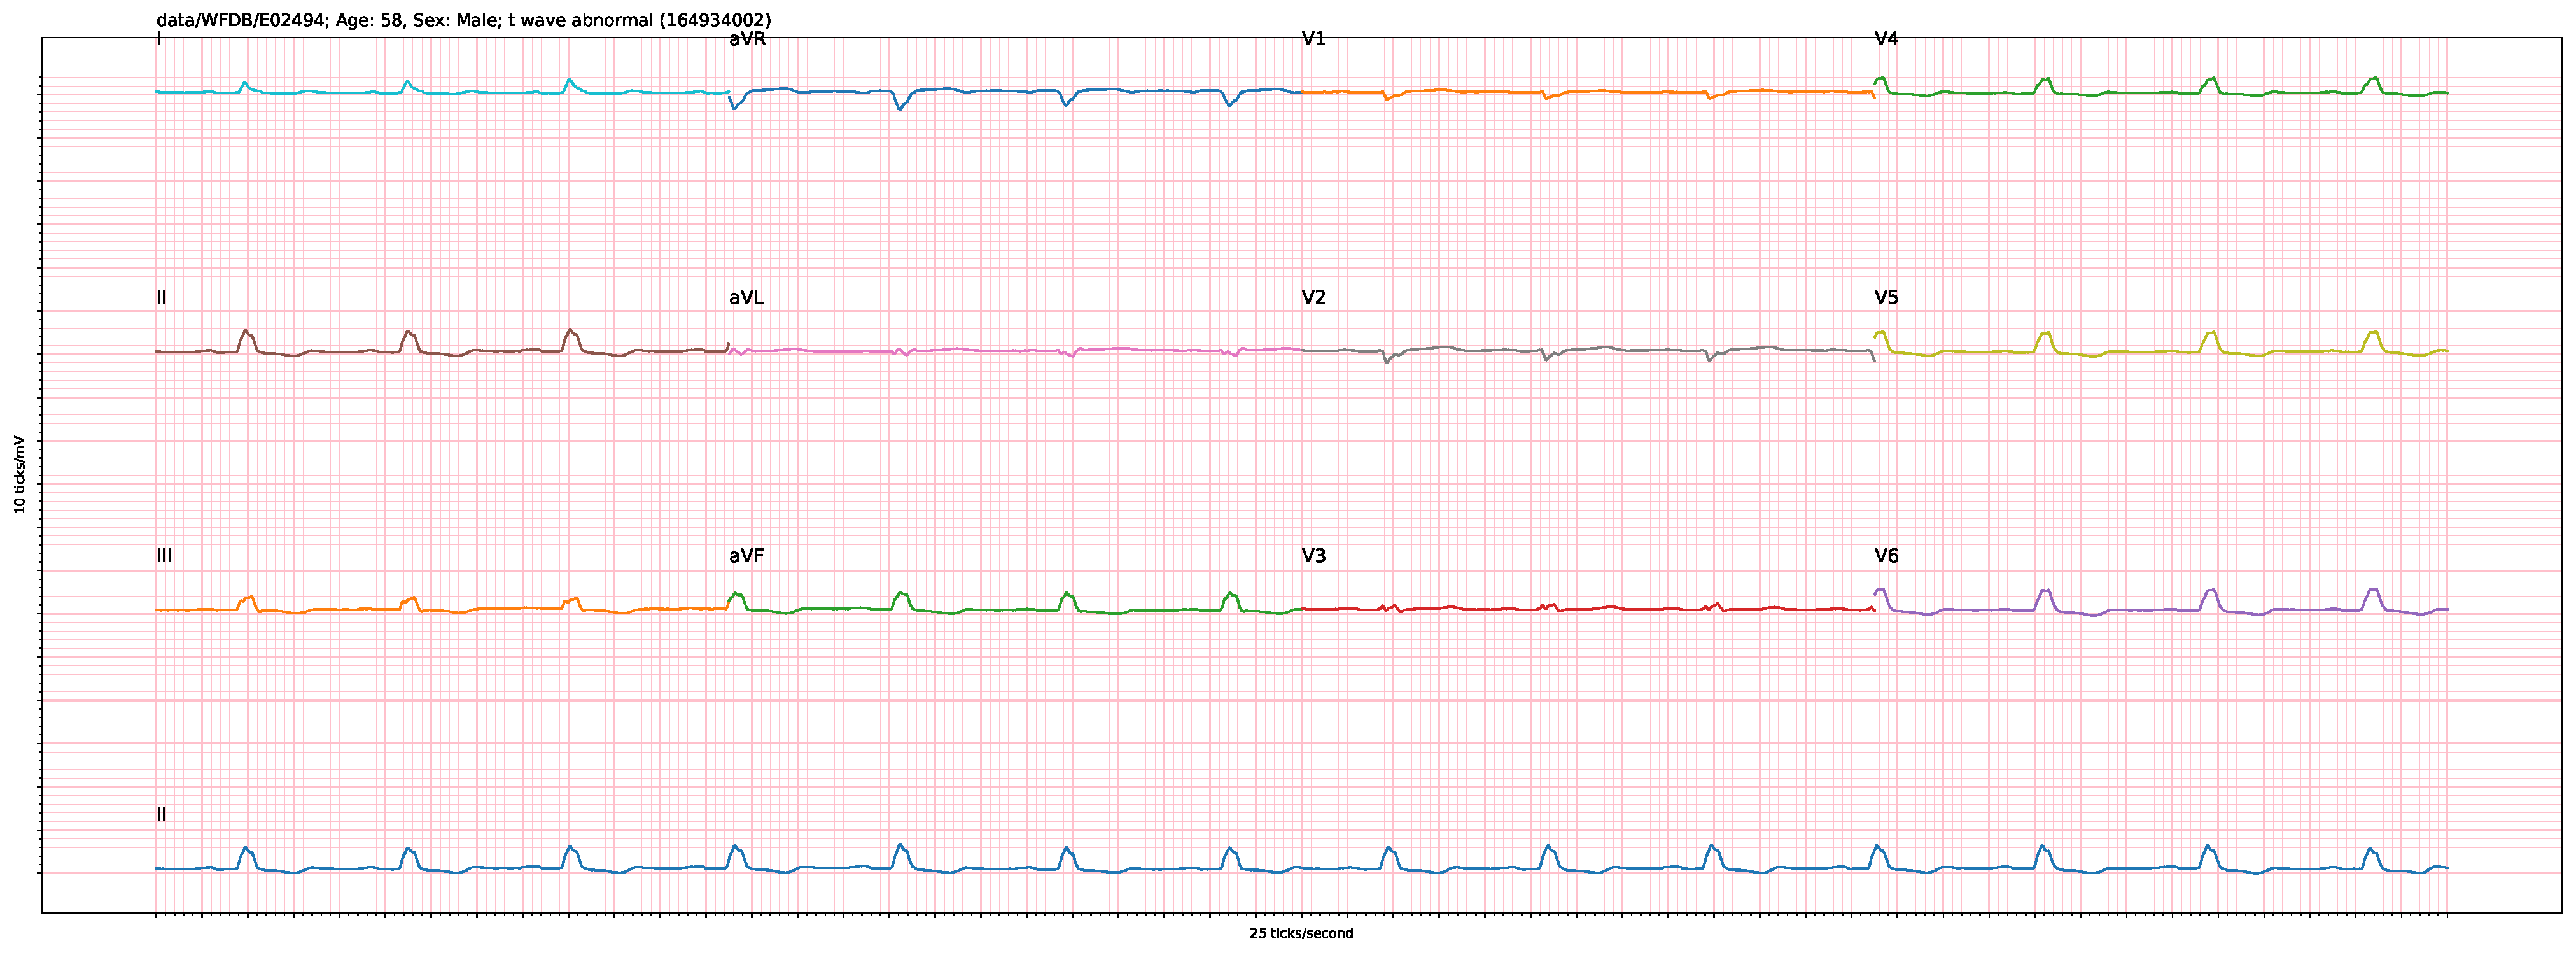
\includegraphics[width=1.2\textwidth]{figure/TAb/full_37_12821.pdf}}
        \caption{Instance of 12-lead \gls{ecg} with abnormal T wave.}
        \label{fig:full_TAb}
    \end{figure}
    \item[\gls{tab}]
    An abnormality in the T wave ranges from low T-wave amplitudes to complete inversion of the T wave. Normal T waves typically align with the QRS complex direction. They should be upright in leads I, II, V3-6, and inverted in lead aVR. Normal T waves are typically asymmetric, with a faster second half compared to the first half~\cite{ecg-utah-lesson}.
    See Figure~\ref{fig:full_TAb} for a reference \gls{ecg} with abnormal T waves.

    \begin{figure}[H]
        \centering
        \makebox[\textwidth][c]{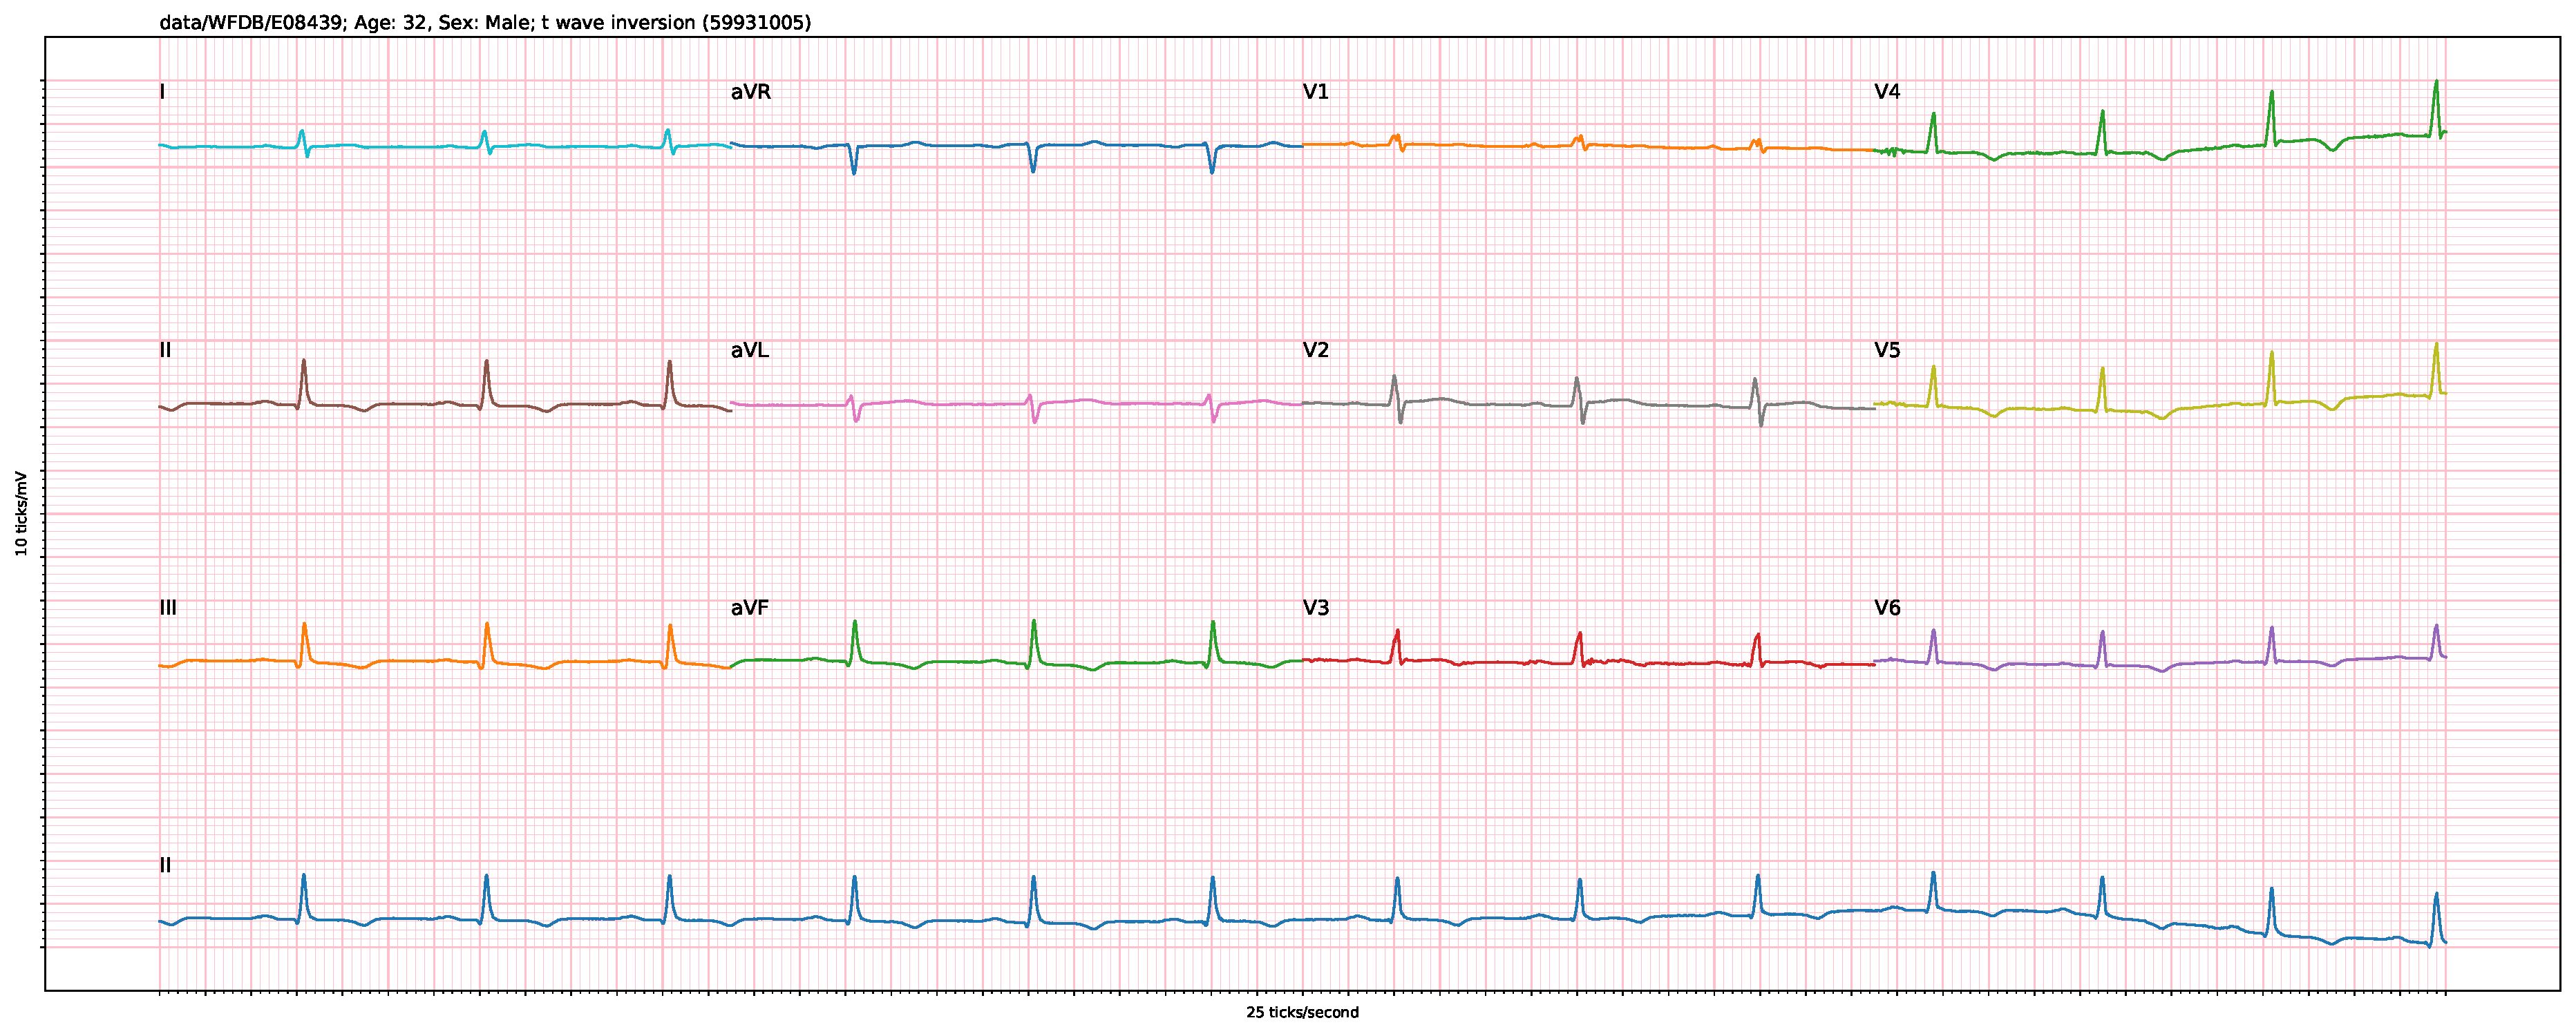
\includegraphics[width=1.2\textwidth]{figure/TInv/full_29_18766.pdf}}
        \caption{Instance of 12-lead \gls{ecg} with T wave inversion. Leads with T waves of incorrect direction are observed in leads II, III, aVR (should be inverted), aVF, and V3-6.}
        \label{fig:full_TInv}
    \end{figure}
    \item[\gls{tinv}] This condition is semantically a more specific form of \gls{tab}, but only evaluating the condition of T wave inversion.
    Figure~\ref{fig:full_TInv} contains a reference \gls{ecg} with inverted T waves.

    \item[\gls{vpb}] This diagnosis is identical to \gls{pvc}.
\end{description}

\subsection{Scoring Function}
\label{ssec:scoring_function}

The \emph{PhysioNet/CinC 2020 Challenge}~\cite{physionet_challenge_2020} rewards partial credit for incorrect classification predictions using a weighted scoring function.
The intention of this scoring function is to weigh predictions that result in similar outcomes or treatments as the ground truth labels more favorably.
The similarity of two classes aim to minimize potential harm of applied treatment, as treatment response may be similar in both cases.

We define a set of diagnoses $C={\{c_i\}}^m_{i=1}, \quad i = 1 \dots n$ for $m$ distinct labels in a corpus of $n$ recordings.
We compute a confusion matrix $A=[a_{ij}]$ such that each cell contains the sum of all $n$ records that are classified as diagnosis $c_i$ and have the ground truth diagnosis of $c_j$, see Equation~\ref{eq:conf_matrix_cell} and Equation~\ref{eq:conf_matrix_cell_cond}.
\begin{equation}
    a_{ij} = \sum^n_{k=1}{a_{ijk}} \label{eq:conf_matrix_cell}
\end{equation}
Due to the multi-label nature of this task, a single \gls{ecg} record may have multiple diagnoses.
The contribution of a single record is normalized by dividing over $|\{x_k \cup y_k \}|$, or the number of classes with a ground truth positive label or classifier output.
\begin{equation}
    a_{ijk} = \left\{\begin{array}{lr}
        \dfrac{1}{|\{x_k \cup y_k \}|} & \text{if } c_i \in x_k \text{ and } c_j \in y_k \\
        0 & \text{otherwise}
    \end{array} \right. \label{eq:conf_matrix_cell_cond}
\end{equation}

\begin{figure}[ht]
    \centering
    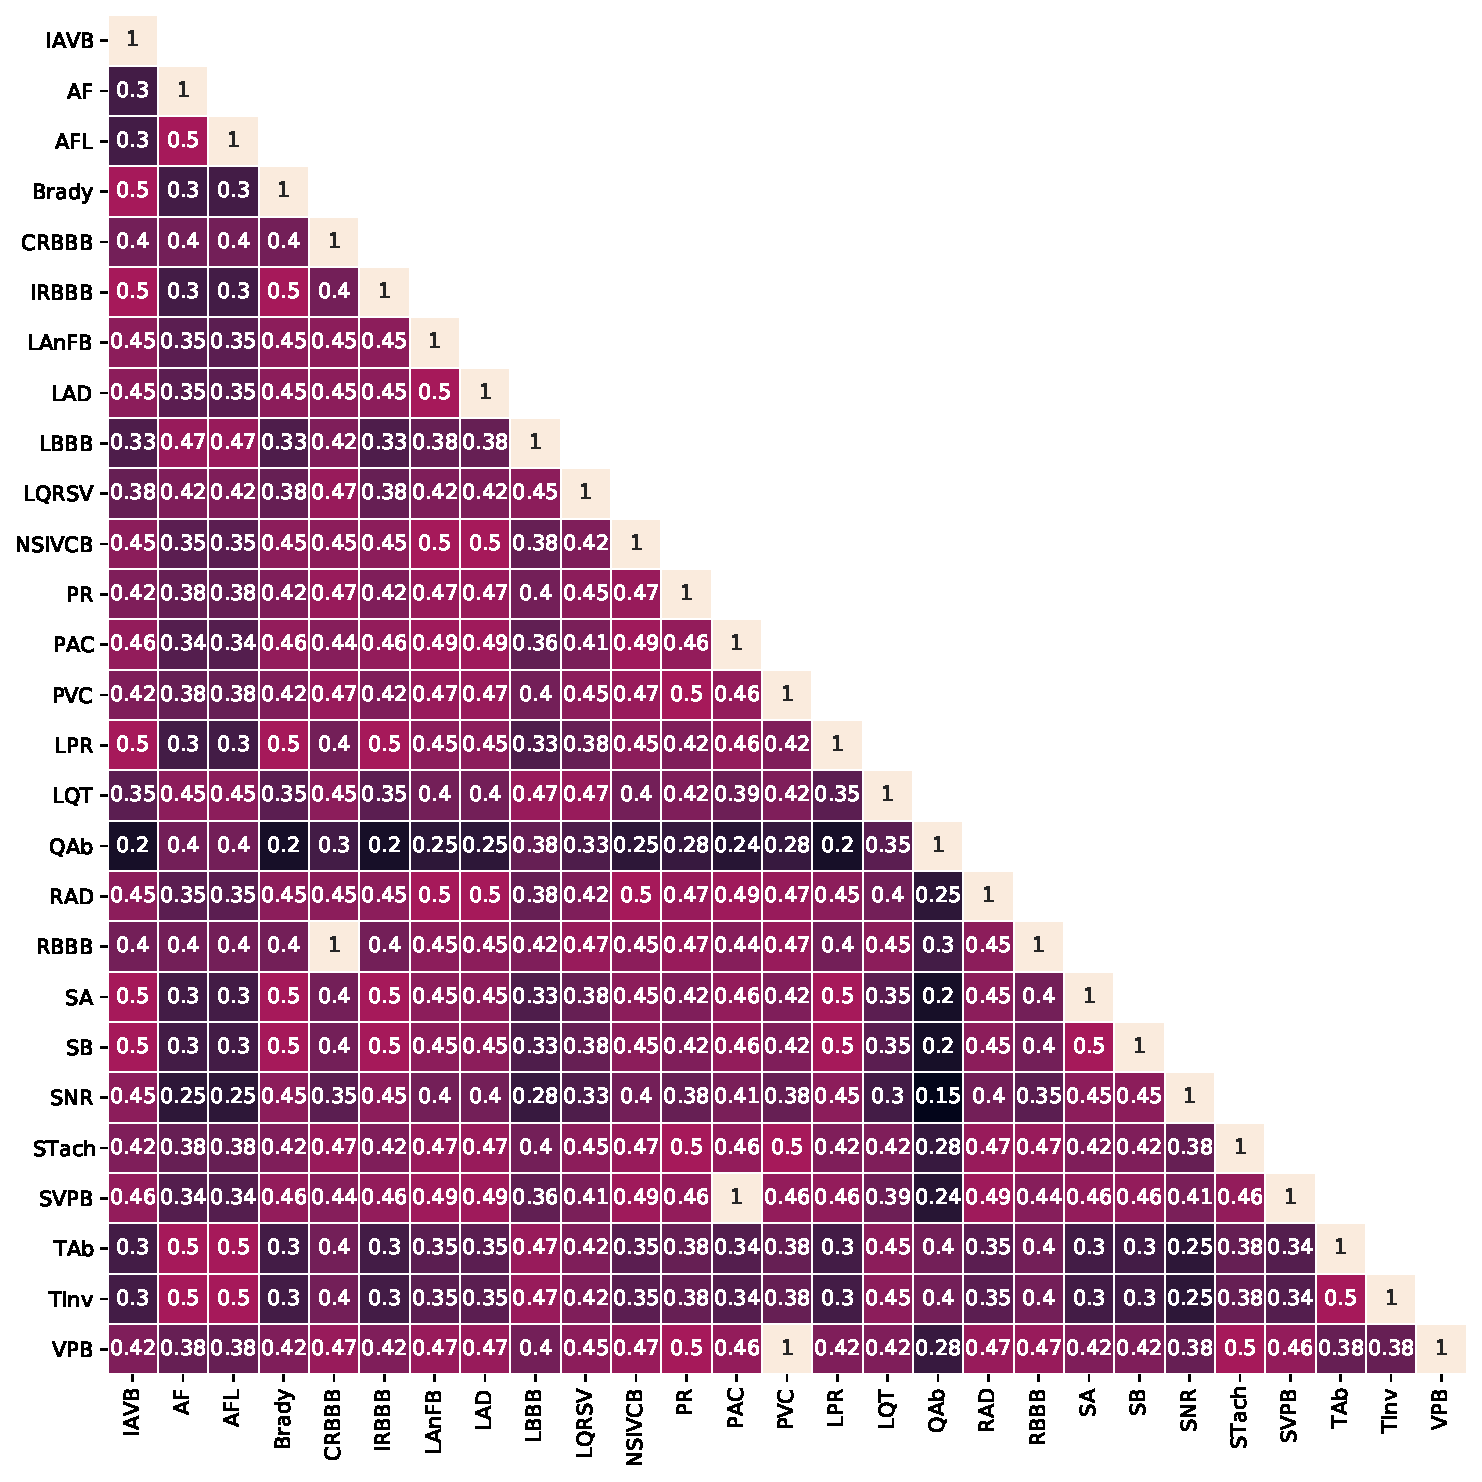
\includegraphics[trim={0.3cm 0.3cm 0.3cm 0.3cm},clip,width=0.8\textwidth]{figure/aenc_label_weights.pdf}
    \caption{PhysioNet/CinC 2020 Challenge~\cite{physionet_challenge_2020} provided reward matrix $W$ for the diagnoses evaluated in the classification task.}
    \label{fig:reward_matrix}
\end{figure}
A matrix of weights $W=[w_{ij}]$ is provided by the challenge organizers to specify the reward for a classifier output of class $c_i$ with a ground truth positive label of $c_j$.
See Figure~\ref{fig:reward_matrix} for a visualization of the provided weights and relationship to the classification labels.

\begin{equation}
    s = \sum_{i=1}^m\sum_{j=1}^m w_{ij}a_{ij} \label{eq:scoring_function}
\end{equation}
The objective of the challenge is to maximize the scoring metric $s$ as defined in Equation~\ref{eq:scoring_function}.
The challenge emphasizes that the reward matrix used $W$ is opinionated and should be tailored to the preferences of the researchers and institutions in future experiments~\cite{physionet_challenge_2020}.

\section{Related Work}
I summarize the \emph{PhysioNet/CinC 2020 Challenge}~\cite{physionet_challenge_2020} successful entrants, emphasizing noteworthy approaches and categorizing the general distribution of the competition strategies.
All of the ranked challenge participants have publicly available papers~\footnote{PhysioNet 2020 successful entrants and papers: \url{https://github.com/physionetchallenges/physionetchallenges.github.io/tree/master/2020/papers}}.
There are also publications that do not have a official phase challenge entry, due to various failures in the remote evaluation and training of the submitted entry.
All in all, there are 41 successful submissions and 62 publications addressing the 12-lead \gls{ecg} classification challenge.

The top ranked entry proposed by Natarajan \emph{et al} combined handcrafted \gls{ecg} features with a deep learning convolutional and transformer neural network model for learned discriminative feature representations~\cite{natarajan2020CINC-multilabel-ECG}.
They initially generated over 300 \gls{ecg} features extracted from lead II, but pruned to 20 derived features using a random forest classifier.
The remaining leads were not used in tabular feature engineering, but were applied to training the transformer neural network.
They achieved a final official phase validation score of $0.587$ with a test score of $0.533$.
Impressively, despite this approach using deep learning techniques and winning the competition, no external datasets were used to pretrain or otherwise enhance the model.

The second ranked entry submitted by Zhao \emph{et al} used an adapted ResNet for the classification of \gls{ecg}s and attained a official phase validation score of $0.672$ and test score of $0.520$~\cite{zhao2020CINC-multilabel-ECG}.
The age and sex meta features were encoded into their final classification layer using one-hot encoding, relying otherwise on learned features from their deep convolutional network.
Additionally, their model was trained on additional data not provided by the official challenge sources.
The third ranked entry proposed by Zhu \emph{et al} also used an adapted ResNet with squeeze-and-excitation blocks and scored a challenge validation score of $0.682$ with a test score of $0.514$~\cite{zhu2020CINC-multilabel-ECG}.
No metadata was used in their classifier, relying only on signal morphology to generate their predictions.

Of all 62 accepted papers, the overwhelming majority of approaches used deep learning as part of their model.
Convolutions were used in 54 (87.1\%) of all challenge papers.
Recurrent neural networks were used in 32 (51.6\%) of the papers, with 17 (27.4\%) of the papers using the long short term memory (LSTM) network variant.
Three (4.8\%) papers used the transformer neural network architecture.
Only 7 (11.3\%) papers opted not to use deep learning at all, relying on manual feature extraction and traditional machine learning approaches like decision trees and support vector machines (our challenge submission being one of these 7 papers).

% \begin{table}
%     \caption{\label{tab:submission_summary} A count summary of the 62 methodological approaches of the \emph{PhysioNet/CinC 2020 Challenge} submitted papers. The methodology defined in a paper may utilize multiple techniques.}
%     \vspace{2 mm}
%     \centerline{\begin{tabular}{@{}ll@{}l@{}r@{}}
%         Count & 
%     \end{tabular}}
% \end{table}

% An analysis of all the publicly available papers is shown in Table~\ref{tab:submission_summary}.

% Due to the rise in popularity of deep learning approaches and the availability of 12-lead \gls{ecg} datasets, deep convolutional neural networks have become the most common model for \gls{ecg} analysis~\cite{ribeiro2020, BALOGLU201923, 8846016, CHEN2020100886, SMITH201988}.

\end{document}
